\documentclass[a4paper,10pt]{report}

\usepackage{graphicx}
\usepackage{subcaption}
\usepackage{booktabs}
\usepackage{polyglossia}
\setdefaultlanguage[spelling=new,babelshorthands=true]{german}
\usepackage{fontspec}
\usepackage{parskip}
\usepackage{amsmath}
\usepackage{amsfonts}
\usepackage[backend=biber,style=numeric,babel=other]{biblatex}
\addbibresource{literatur.bib}
\usepackage[hidelinks]{hyperref}
\usepackage[left=2cm,right=2cm,top=3.0cm,bottom=3.0cm]{geometry}
\usepackage[arrow, matrix, curve]{xy}
\usepackage{msc}
\usepackage{float}
\usepackage{xcolor}
\usepackage[edges]{forest}
\usepackage{tikz}
\usetikzlibrary{positioning, arrows.meta, fit, backgrounds, decorations.pathreplacing}
\tikzset{
    archbox/.style   = {draw, rounded corners=2pt, align=center, inner sep=5pt,
                        minimum height=1.05cm, font=\small},
    extern/.style    = {archbox, fill=black!5},
    device/.style    = {archbox, fill=black!12, thick},
    modul/.style     = {archbox, fill=black!3, minimum width=3.3cm},
    huelle/.style    = {draw, dashed, rounded corners=4pt, inner sep=9pt},
    link/.style      = {-{Latex[length=2.2mm]}, thick},
    funk/.style      = {link, dashed},
    beschr/.style    = {font=\footnotesize, align=center, inner sep=2pt}
}
\usepackage{listings}
\lstset{
    language=Python,
    basicstyle=\ttfamily\small,
    keywordstyle=\color{purple}\bfseries,
    commentstyle=\color{gray}\itshape,
    stringstyle=\color{teal},
    numberstyle=\tiny\color{gray!60},
    identifierstyle=\color{black},
    backgroundcolor=\color{gray!5},
    frame=single,
    frameround=tttt,
    framerule=0.5pt,
    framexleftmargin=5pt,
    breaklines=true,
    showstringspaces=false,
    numbers=left,
    numbersep=10pt,
    tabsize=4,
    captionpos=b,
    xleftmargin=10pt,
    xrightmargin=5pt,
    emphstyle=\color{blue!80!black},
    emph={def,class,import,from,as,return,if,elif,else,for,while,try,except,with}
}
%\usepackage{draftwatermark}
%\SetWatermarkText{Entwurf}
%\nofiles

\begin{document}

% Deckblatt
\begin{titlepage}
    \vbox{ }
    \vbox{ }
    \begin{center}
% Upper part of the page

        
\includegraphics[width=0.50\textwidth]{Images/HTWK_Zusatz_de_V_Black}\\[1cm]
        
\includegraphics[width=0.30\textwidth]{Images/HTWK-Fakultaetszusatz_im_schwarz_de}\\[1cm]
        
        \vfill
        {\Large Abschlussarbeit zur Erlangung des akademischen Grades}\\[20pt]
        {\Large Bachelor of Science (B.Sc.)}\\[20pt]
        {\Large im Studiengang Bachelor Informatik}\\[10pt]
        {\Large der Fakultät Informatik und Medien}\\[20pt]
        \vbox{}

% Title
        {\LARGE \textbf{Entwicklung eines Beleuchtungssystems}}\\[10pt]
        {\LARGE \textbf{für Veranstaltungen als LED-Leuchtröhren}}\\[10pt]
        {\LARGE \textbf{mit funkgestützter Signalübertragung}}\\[40pt]
        {\Large Rami Hoßbach}\\[10pt]
        {\Large Leipzig, den \today}\\[20pt]
        \vfill

% Bottom of the page
        \begin{tabular}{l l}
            \Large Erstgutachter:  & \Large Prof. Dr.-Ing. Jens Wagner\\[10pt]
            \Large Zweitgutachter: & \Large M.Sc. Marian Ulbricht\\
        \end{tabular}
    \end{center}
\end{titlepage}


%Abstract
\newpage
\begin{abstract}
Diese Arbeit befasst sich mit der Entwicklung und experimentellen Untersuchung eines Beleuchtungssystems für Veranstaltungen, das aus LED-Leuchtröhren mit funkgestützter Übertragung der Steuersignale besteht.
Ausgangspunkt ist der erhebliche Aufwand, den die Signalverkabelung nach dem DMX512-Standard bei temporären und häufig wechselnden Aufbauten verursacht, sowie die Lücke zwischen funktional umfassenden, jedoch kostenintensiven Premiumsystemen und preisgünstigen Alternativen mit deutlich reduziertem Funktionsumfang.
Ziel ist ein offengelegtes und nachbaubares System, das Funkempfang, Energieversorgung und pixelgenaue Ansteuerung im Leuchtmittel selbst vereint und die Signalverkabelung dadurch vollständig entfallen lässt.

Zur Umsetzung wurde eine Bridge auf Basis eines ESP32 entwickelt, die Steuerdaten aus einer bestehenden Lichtinfrastruktur über DMX512 entgegennimmt oder in einem eigenständigen Modus selbst erzeugt und über das Protokoll ESP-NOW als Broadcast an die Leuchtröhren verteilt.
Da das Verfahren im Broadcast-Betrieb keine Zustellgarantie bietet, wird auf einen Rückkanal verzichtet und jeder Datenstand stattdessen mehrfach ausgesendet.
Neben der Firmware beider Gerätetypen umfasst die Arbeit den Entwurf der Leiterplatten sowie der Gehäuse sämtliche Entwurfsdaten werden unter einer freien Lizenz veröffentlicht.
Sämtliche Projektdateien sind unter \url{https://github.com/nichtrami/led_tube} frei zugänglich.

Die Bewertung der Funkstrecke erfolgt über Messreihen von jeweils 300\,s, die mit der Zielhardware und dem produktiven Sendepfad erhoben wurden.
Untersucht wurden eine Referenzmessung unter Idealbedingungen, zwei Reichweitenmessreihen mit und ohne Sichtverbindung über Distanzen bis 200\,m sowie der Betrieb unter realer Fremdfunklast.
Als Bewertungsgrößen dienen der Anteil vollständig verlorener Sequenzwerte, die mittlere Anzahl empfangener Kopien je Sequenzwert als verbleibende Fehlerreserve sowie die Länge zusammenhängender Verlustserien.

Unter Idealbedingungen wurde kein einziger von 23\,984 übertragenen Sequenzwerten verloren.
Die geforderte Mindestreichweite von 50\,m wird mit freier Sicht bei 0,06\,\% Sequenzverlust und ohne Sichtverbindung bei 2,08\,\% erreicht, die vollständige Abschattung durch eine Stahlbetonstütze kostet dabei etwa den Faktor zwei der nutzbaren Distanz.
Unter erhöhter Fremdfunklast bleibt der Verlust mit 0,51\,\% gering, enthält jedoch eine zusammenhängende Unterbrechung von 750\,ms, die auf die Konkurrenz um den Übertragungskanal zurückgeht.
Die Empfangsredundanz erweist sich in allen Messreihen als früher Indikator einer sich verschlechternden Verbindung, da sie bereits messbar sinkt, während der Sequenzverlust noch nahezu bei null liegt.

Das entwickelte System erfüllt die gestellten Anforderungen an Aktualisierungsrate, Reichweite und Zuverlässigkeit im vorgesehenen Einsatzbereich bei Materialkosten von rund 62\,€ je Leuchtröhre.
Die Arbeit leistet damit einen Beitrag zur drahtlosen Ansteuerung verteilter eingebetteter Aktoren unter realen Umgebungsbedingungen und stellt zugleich eine reproduzierbar dokumentierte, quelloffene Alternative zu kommerziellen Systemen bereit.
\end{abstract}

\newpage
\null
\thispagestyle{empty}
\newpage


% Inhaltsverzeichnis
\setcounter{page}{1}
\pagenumbering{arabic}
\tableofcontents

%Leere Seite
\newpage
\null
\newpage

% Kapitel einbinden
\chapter{Einleitung}
\label{chap:einleitung}

\section{Motivation}
\label{sec:motivation}

Bühnenbeleuchtung ist ein zentraler Bestandteil moderner Theater-, Konzert- und
Veranstaltungsproduktionen. Durch gezielte Lichtgestaltung können Atmosphäre,
Stimmungen und visuelle Effekte erzeugt werden, die wesentlich zur Wahrnehmung
einer Aufführung durch das Publikum beitragen. Neben der rein funktionalen
Ausleuchtung der Bühne ermöglicht die Lichttechnik somit eine kreative und
dramaturgische Gestaltung des gesamten Bühnengeschehens.

Zur Steuerung professioneller Beleuchtungssysteme hat sich in der
Veranstaltungstechnik das Protokoll DMX (Digital Multiplex) als De-facto-Standard
etabliert. DMX erlaubt die zentrale Steuerung einer Vielzahl von
Beleuchtungsgeräten über ein standardisiertes Kommunikationsprotokoll und bietet
eine zuverlässige sowie flexible Möglichkeit zur Echtzeitsteuerung komplexer
Lichtinstallationen.

Die Signalführung dieses Standards ist jedoch kabelgebunden: Jedes
Beleuchtungsgerät muss über eine eigene Leitung in eine durchgehende DMX-Kette
eingebunden werden. Vor allem bei temporären Installationen, mobilen Bühnen oder
häufig wechselnden Aufbauten wird die dafür erforderliche Verkabelung zu einem
wesentlichen Komplexitätsfaktor. Vor diesem Hintergrund entsteht ein Interesse an
flexibleren Lösungen, die den Verkabelungsaufwand bei gleichbleibender
Funktionalität verringern.

\section{Problemstellung}
\label{sec:problemstellung}

Die kabelgebundene Signalübertragung bietet eine hohe Zuverlässigkeit, führt in
der Praxis jedoch zu drei Nachteilen, die den Einsatz insbesondere außerhalb
fester Installationen erschweren.

Der erste betrifft Zeit und Personal. Die Signalverkabelung erfordert eine
sorgfältige Planung sowie die manuelle Verbindung sämtlicher Beleuchtungsgeräte
innerhalb der DMX-Kette. Bei größeren Installationen entsteht dadurch ein
erheblicher Zeitaufwand beim Auf- und Abbau, der zudem Personal mit
entsprechender Erfahrung im Umgang mit Veranstaltungstechnik voraussetzt.

Der zweite Nachteil ist materieller Art. Kabel und Verbindungselemente
verursachen Kosten für Anschaffung, Wartung und Transport und müssen in
ausreichender Länge und Anzahl vorgehalten werden. Mit der Zahl der Verbindungen
steigt darüber hinaus die Zahl möglicher Fehlerquellen, was die Fehlersuche im
laufenden Betrieb erschwert.

Der dritte Nachteil liegt im verfügbaren Angebot. Zwar existieren bereits
kommerzielle Lösungen zur drahtlosen Übertragung von DMX-Daten, diese sind jedoch
häufig mit hohen Anschaffungskosten verbunden und richten sich primär an
professionelle Großproduktionen. Für kleinere Produktionen, experimentelle
Bühneninstallationen oder flexible Lichtsysteme stehen daher nur begrenzt
kostengünstige und zugleich leistungsfähige Lösungen zur Verfügung.

\section{Zielsetzung}
\label{sec:zielsetzung}

Ziel dieser Arbeit ist die Entwicklung eines Beleuchtungssystems für
Veranstaltungen, das DMX-Steuersignale drahtlos an mehrere Leuchteinheiten
überträgt. Diese werden in Form von LED-Leuchtröhren realisiert, die die
empfangenen Steuerdaten unmittelbar in Lichtsignale umsetzen. Ein zentrales
Element bildet eine sogenannte Bridge, welche die Steuerdaten aus einer
bestehenden Lichtinfrastruktur entgegennimmt und an die Leuchtröhren verteilt.
Die Arbeit umfasst dabei sowohl die Hardware als auch die Software beider
Gerätetypen.

Ein wesentliches Entwicklungsziel ist die Gewährleistung einer stabilen
Datenübertragung mit hinreichender Aktualisierungsrate und zeitlicher Konstanz,
sodass die zeitkritischen Anforderungen der Lichtsteuerung erfüllt werden. Dies
schließt die robuste Funktion unter praxisnahen Bedingungen mit potenziellen
Funkstörungen ausdrücklich ein.

Darüber hinaus soll der Nachbau des Systems niedrigschwellig möglich sein.
Vorgesehen sind deshalb ausschließlich frei zugängliche Komponenten, sodass auch
Anwenderinnen und Anwender mit geringen Vorkenntnissen den Aufbau bewältigen
können. Diesem Ziel folgt auch die Ausrichtung als Open-Source-Projekt: Neben der
Software werden die Platinenlayouts der Elektronikbaugruppen sowie die 3D-Modelle
der Gehäuse veröffentlicht. Damit sollen Transparenz geschaffen, die
Nachvollziehbarkeit technischer Entscheidungen verbessert und die
Weiterentwicklung durch Dritte erleichtert werden.

\section{Wissenschaftliche und praktische Relevanz}
\label{sec:wissenschaftliche-und-praktische-relevanz}

Die Kommunikation in verteilten eingebetteten Systemen ist ein relevantes
Forschungsfeld innerhalb der Informatik. Zuverlässigkeit, Latenzverhalten,
Skalierbarkeit und Robustheit unter realen Einsatzbedingungen stellen dabei
zentrale Fragestellungen dar. Das entwickelte System realisiert ein solches
verteiltes eingebettetes Echtzeitsystem zur Steuerung von Aktoren und erlaubt es
damit, Entwurfsentscheidungen, Leistungsgrenzen und Zielkonflikte zwischen
Flexibilität, Komplexität und Übertragungsqualität systematisch zu untersuchen.
Von besonderem Interesse ist die Frage, welche Zuverlässigkeit eine
unidirektionale Funkstrecke ohne Zustellbestätigung unter realen
Umgebungsbedingungen erreicht.

Praktisch adressiert die Arbeit genau jenen Anwendungsbereich, für den nach
Abschnitt~\ref{sec:problemstellung} bislang keine geeignete Lösung verfügbar ist.
Da sämtliche Entwurfsdaten offengelegt werden, ist das Ergebnis nicht nur
nachvollziehbar, sondern auch unmittelbar nachnutzbar.

\section{Aufbau der Arbeit}
\label{sec:aufbau-der-arbeit}

Kapitel~\ref{chap:grundlagen} stellt die theoretischen Grundlagen zu
eingebetteten Systemen, den verwendeten Kommunikationsprotokollen und der
drahtlosen Übertragung vor. Kapitel~\ref{chap:stand-der-technik} ordnet die
Arbeit in den Stand der Technik ein, indem kommerzielle Systeme und verwandte
wissenschaftliche Arbeiten betrachtet und die bestehenden Lücken benannt werden.

Auf dieser Grundlage leitet Kapitel~\ref{chap:anforderungsanalyse} die
funktionalen und nicht-funktionalen Anforderungen ab.
Kapitel~\ref{chap:systemarchitektur} beschreibt daraufhin die Architektur des
Systems einschließlich der Hardware- und Softwarekomponenten von Bridge und
Leuchtröhren, während Kapitel~\ref{chap:implementierung} deren konkrete Umsetzung
darlegt.

Kapitel~\ref{chap:evaluierung} untersucht das entwickelte System experimentell.
Erhoben werden Messreihen zur Verbindungsstabilität, zur Aktualisierungsrate und
zur Zuverlässigkeit der Übertragung, die anschließend den Anforderungen
gegenübergestellt werden. Kapitel~\ref{chap:diskussion-und-ausblick} bewertet die
Ergebnisse, zieht ein Fazit und zeigt Ansätze für zukünftige Weiterentwicklungen
auf.

\chapter{Theoretische Grundlagen}
\label{chap:grundlagen}

\section{Eingebettete Systeme}
\label{sec:eingebettete-systeme}

Eingebettete Systeme werden von Marwedel als informationsverarbeitende Systeme 
definiert, die in in ein umgebendes Produkt eingebettet sind und dort dedizierte 
Steuerungs-, Regelungs- oder Überwachungsaufgaben übernehmen \cite{marwedel2021}. 
Im Gegensatz zu universellen Computersystemen sind sie auf einen konkreten 
Anwendungsfall zugeschnitten. Als gemeinsame Merkmale dieser Systemklasse nennt 
Marwedel insbesondere Echtzeitanforderungen sowie Anforderungen an Verlässlichkeit 
und Effizienz \cite{marwedel2021}, letztere äußert sich in ressourcensparender 
Hardware und häufig energiesparenden Betriebsweisen.

Die zunehmende Miniaturisierung und Leistungsfähigkeit moderner Mikrocontroller hat in 
den vergangenen Jahren zu einer breiten Durchdringung eingebetteter Systeme in 
unterschiedlichen Domänen geführt. Insbesondere die 
Integration drahtloser Kommunikationsschnittstellen wie WLAN und Bluetooth in 
kostengünstige Mikrocontroller-Plattformen eröffnet neue Möglichkeiten für verteilte, 
vernetzte Systemarchitekturen.

Im Kontext des entwickelten LED-Tube-Systems bilden eingebettete Systeme die zentrale 
Komponente sowohl der Bridge als auch der einzelnen Tubes. Beide setzen auf den 
ESP32-Mikrocontroller, der im Folgenden näher betrachtet wird.

\subsection{ESP32-Mikrocontroller}
\label{subsec:esp32}

Die Bezeichnung ESP32 steht nicht für einen einzelnen Chip, sondern für eine von 
Espressif Systems entwickelte Familie von System-on-Chips (SoC), deren Mitglieder sich 
in Prozessorarchitektur, Speicherausstattung und Peripherie unterscheiden 
\cite{espressif_esp32}. Kennzeichnend für die gesamte Familie ist die Integration eines 
leistungsfähigen Prozessors und umfangreicher drahtloser Kommunikationsschnittstellen 
(WLAN 802.11 b/g/n sowie Bluetooth beziehungsweise Bluetooth Low Energy) auf einem 
einzigen Baustein. Das namensgebende erste Mitglied der Familie kombiniert dabei einen 
Dual-Core-Prozessor des Typs Xtensa LX6 mit WLAN und Bluetooth 4.2. Seit der Einführung 
im Jahr 2016 hat sich die ESP32-Reihe zu einer der meistverwendeten Plattformen im 
Bereich des Internet of Things (IoT) und eingebetteter Systeme entwickelt. Besonders die 
Kompatibilität mit dem im Hobby- und Maker-Bereich weit verbreiteten Arduino-Ökosystem 
sowie die umfassende Unterstützung durch die Entwicklergemeinschaft haben zur 
Popularität des ESP32 beigetragen.

\subsubsection{Technische Merkmale}
\label{subsubsec:esp32-merkmale}

Es existieren verschiedene Varianten des ESP32, die sich in Bezug auf Speicherkapazität, Anzahl der GPIO-Pins,
integrierte Peripheriefunktionen und unterstützte Kommunikationsschnittstellen unterscheiden.
Die in diesem Projekt verwendeten Varianten verfügen über zwei unabhängige 32-Bit-Prozessorkerne mit einer maximalen 
Taktfrequenz von bis zu 240\,MHz. Diese Dual-Core-Architektur ermöglicht es, 
rechenintensive Aufgaben wie Signalverarbeitung und drahtlose Kommunikation parallel 
auszuführen.

Neben den Kommunikationsschnittstellen bieten die Bausteine der Familie umfangreiche 
Peripheriefunktionen, darunter mehrere UART-, SPI- und I²C-Schnittstellen, 
GPIO-Pins (General Purpose Input/Output), ADCs (Analog-Digital-Wandler), PWM-Kanäle 
(Pulse Width Modulation) sowie kapazitive Berührungssensoren \cite{espressif_esp32}. 

\subsubsection{Software-Entwicklung und Ökosystem}
\label{subsubsec:esp32-software}

Espressif Systems stellt mit dem ESP-IDF (Espressif IoT Development Framework) eine 
umfassende Entwicklungsumgebung bereit, die auf dem FreeRTOS-Echtzeitbetriebssystem 
basiert und native Unterstützung für C/C++-Programmierung bietet. Daneben existiert eine 
breite Community-Unterstützung für alternative Entwicklungsumgebungen wie Arduino IDE, 
PlatformIO sowie MicroPython.

Die Integration des ESP32 in Entwicklungsumgebungen sowie die Verfügbarkeit 
zahlreicher Open-Source-Bibliotheken haben die Einstiegshürde deutlich gesenkt und den 
Einsatz des Mikrocontrollers sowohl im Amateur- als auch im industriellen Kontext 
gefördert.

\subsubsection{Einsatz im entwickelten System}
\label{subsubsec:esp32-system}

Im Rahmen dieser Arbeit bildet der ESP32 die hardwaretechnische Grundlage sowohl für die 
zentrale Bridge als auch für die dezentralen LED-Tubes. Die Dual-Core-Architektur 
ermöglicht die parallele Verarbeitung von Netzwerkkommunikation (ESP-NOW, Art-Net) auf 
einem Kern und die Ansteuerung der LED-Hardware auf dem zweiten Kern.

Die integrierte WLAN-Funktionalität wird für die Implementierung des proprietären 
ESP-NOW-Protokolls genutzt, welches die drahtlose Datenübertragung zwischen Bridge und 
Tubes realisiert. Gleichzeitig erlaubt die Ethernet-Erweiterbarkeit über externe Module 
die Anbindung der Bridge an professionelle Lichtsteuersysteme mittels Art-Net.

Die GPIO-Pins dienen der Ansteuerung der Peripheriekomponenten, etwa der LED-Strips und 
der übrigen in der Schaltung verbauten ICs (Integrated Circuits).
Die Leistungsfähigkeit des ESP32 stellt sicher, dass die zeitkritischen Anforderungen der Lichtsteuerung erfüllt werden können, 
während gleichzeitig die Flexibilität für eventuelle zukünftige Erweiterungen gegeben ist.

\section{Kommunikationsprotokolle}
\label{sec:kommunikationsprotokolle}

\subsection{DMX512}
\label{subsec:dmx512}

DMX512 (Digital Multiplex 512) ist ein weit verbreiteter Industriestandard für die
Steuerung von Bühnen- und Veranstaltungstechnik. Der Standard wurde 1986 vom United 
States Institute for Theatre Technology (USITT) entwickelt und wird heute von der 
Entertainment Services and Technology Association (ESTA) gepflegt. Er wurde seither in 
mehreren Revisionen fortgeschrieben die aktuelle Fassung ist ANSI E1.11-2024 
\cite{ANSI_E1.11_2024}.

\subsubsection{Technische Grundlagen}
\label{subsubsec:dmx512-technik}

DMX512 überträgt Daten seriell und unidirektional über eine differentielle
RS-485-Leitung mit einer Datenrate von 250\,kbit/s \cite{ANSI_E1.11_2024}. Die
Übertragung erfolgt in Form von Paketen, die neben dem einleitenden START-Code bis zu
512 Datenfelder (Slots) umfassen. Jeder Slot wird durch einen 8-Bit-Wert (0--255)
repräsentiert, der beispielsweise die Helligkeit, Farbe oder Position eines Geräts
definiert.

Die physikalische Verbindung erfolgt über eine Daisy-Chain-Topologie, bei der die Geräte
in Reihe geschaltet werden. Der Standard schreibt vor, die Leitung abzuschließen, um
Reflexionen und die daraus folgenden Fehlfunktionen zu vermeiden als Abschluss ist ein
Widerstand von 120\,Ohm vorgesehen. Die Belastung einer DMX512-Linie ist zudem auf 32
Unit Loads begrenzt, wobei jeder Empfängereingang höchstens eine Unit Load darstellen
darf \cite{ANSI_E1.11_2024}. Größere Installationen erfordern daher Verstärker
(DMX-Splitter), die zugleich die nutzbare Leitungslänge erhöhen. Eine maximale
Leitungslänge legt der Standard selbst nicht fest, sie ergibt sich aus den elektrischen
Eigenschaften der RS-485-Strecke und liegt in der Praxis im Bereich einiger hundert
Meter.

\subsubsection{Protokollstruktur}
\label{subsubsec:dmx512-protokoll}

Ein DMX512-Paket beginnt mit einer Reset-Sequenz aus \textit{Break}, einer Unterbrechung
der Datenleitung, dem darauf folgenden \textit{Mark After Break} (MAB) und dem
\textit{START-Code}. Der START-Code kennzeichnet die Art der nachfolgenden Daten für
Beleuchtungsdaten ist der NULL-START-Code mit dem Wert 0x00 vorgesehen. Anschließend
folgen bis zu 512 Datenslots. Für die Zeiten der Reset-Sequenz unterscheidet der
Standard zwischen Sende- und Empfangsseite: Sender müssen einen Break von mindestens
92\,µs und einen MAB von mindestens 12\,µs erzeugen, während Empfänger bereits einen
Break ab 88\,µs und einen MAB ab 8\,µs als Paketbeginn erkennen müssen
\cite{ANSI_E1.11_2024}. Für die Implementierung des Empfängers ist somit die geringere,
für die des Senders die höhere Vorgabe maßgeblich.

Aus Datenrate und Paketaufbau ergibt sich für ein vollständiges Paket mit 513 Slots eine
minimale Aktualisierungszeit von 22,7\,ms und damit eine maximale Wiederholrate von
44\,Hz \cite{ANSI_E1.11_2024} werden weniger Slots übertragen, steigt die erreichbare
Rate entsprechend. Eine bidirektionale Kommunikation ist im regulären Datenpfad nicht
vorgesehen, sodass der Sender keine Rückmeldung über den Status der Empfangsgeräte
erhält.

\subsubsection{Einsatz in der Veranstaltungstechnik}
\label{subsubsec:dmx512-einsatz}

DMX512 hat sich als De-facto-Standard in der professionellen Lichtsteuerung etabliert
und wird von nahezu allen Herstellern unterstützt. Die Einfachheit des Protokolls sowie
die deterministischen Übertragungseigenschaften machen es besonders geeignet für
zeitkritische Anwendungen, bei denen eine zuverlässige Steuerung
erforderlich ist.

Im Kontext des entwickelten LED-Tube-Systems dient der Aufbau des DMX512-Pakets als
Vorbild für das interne Datenformat, in dem die Steuerbefehle repräsentiert werden. Die Bridge kann DMX-Daten sowohl über Art-Net 
(Ethernet) als auch über eine DMX-Schnittstelle (XLR) empfangen und verarbeitet 
diese anschließend zur Übertragung an die LED-Tubes. Dabei bildet die Struktur des 
DMX512-Frames die Grundlage für das entwickelte drahtlose Übertragungsprotokoll, das 
über ESP-NOW an die Tubes übertragen wird. 
Die Orientierung an diesem etablierten Standard ermöglicht eine nahtlose Integration in 
bestehende Lichtsteuersysteme und gewährleistet Kompatibilität mit professioneller 
Steuerungssoftware.


\subsection{Art-Net}
\label{subsec:artnet}

Art-Net ist ein Ethernet-basiertes Kommunikationsprotokoll, das von Artistic Licence
entwickelt wurde und die Übertragung von DMX512-Daten über IP-Netzwerke ermöglicht.
Seit seiner Einführung im Jahr 1998 hat sich Art-Net zu einem weit verbreiteten Standard
in der professionellen Lichtsteuerung entwickelt und wird von zahlreichen
Softwarelösungen und Hardwarekomponenten unterstützt.

Die Etablierung von Art-Net als De-facto-Standard in der professionellen 
Veranstaltungstechnik ist auf die Limitierung klassischer DMX512-Verbindungen 
zurückzuführen. Während eine einzelne DMX-Linie lediglich 512 Kanäle/Byte bereitstellt, 
erfordern moderne Installationen mit einer Vielzahl komplexer Scheinwerfer, 
LED-Pixelmatrizen oder hochauflösenden LED-Wänden häufig mehrere tausend Steuerkanäle. 
Die Art-Net-4-Spezifikation sieht ein theoretisches Maximum von 32.768 DMX-Universen 
vor, wie viele davon tatsächlich übertragen werden können, hängt von der verfügbaren 
Netzwerkbandbreite und der Leistungsfähigkeit der beteiligten Geräte ab 
\cite{artnet4}. Art-Net adressiert damit die gestiegenen Bandbreitenanforderungen 
professioneller Lichtinstallationen. Insbesondere bei der Ansteuerung von LED-Pixelmonitoren, 
bei denen jeder einzelne Pixel mehrere DMX-Kanäle (typischerweise RGB oder RGBW) 
beansprucht, stößt klassisches DMX512 schnell an seine Grenzen, während Art-Net eine 
skalierbare Lösung bietet.

\subsubsection{Funktionsweise und Architektur}
\label{subsubsec:artnet-funktion}

Art-Net kapselt DMX512-Daten in UDP-Pakete (User Datagram Protocol) und überträgt diese
über ein Standard-Ethernet-Netzwerk. Während eine DMX512-Linie auf ein einzelnes
RS-485-Segment mit einem Universum von 512 Kanälen beschränkt ist, ermöglicht Art-Net die
gleichzeitige Übertragung mehrerer Universen über eine einzige Netzwerkverbindung.

Ein Art-Net-Netzwerk besteht typischerweise aus einem oder mehreren \textit{Controllern}
(z.\,B. Lichtsteuerungssoftware), die Art-Net-Pakete senden, sowie \textit{Nodes}, die
diese Pakete empfangen und in DMX512-Signale umwandeln. Die Nodes können dabei sowohl
als Sender als auch als Empfänger fungieren, wodurch bidirektionale Kommunikation
möglich ist.

\subsubsection{Protokollstruktur}
\label{subsubsec:artnet-protokoll}

Jedes Art-Net-Paket beginnt mit einer acht Byte langen, nullterminierten Kennung, 
gefolgt von einem OpCode, der den Pakettyp bestimmt, der
Protokollversion sowie weiteren Verwaltungsinformationen \cite{artnet4}. Das Ziel wird
über die Port-Address adressiert, eine 15\,Bit breite Zahl, die sich aus den
Feldern Net, Sub-Net und Universe34 zusammensetzt und die 32.768 möglichen Universen
abbildet \cite{artnet4}. Der Nutzdatenbereich umfasst bis zu 512 Byte, entsprechend
einem DMX512-Universum.

\subsubsection{Vorteile gegenüber klassischem DMX512}
\label{subsubsec:artnet-vorteile}

Durch die Nutzung von Ethernet-Infrastruktur bietet Art-Net mehrere Vorteile gegenüber
klassischem DMX512:
\begin{itemize}
    \item \textbf{Skalierbarkeit:} Mehrere DMX-Universen können parallel über eine
          einzige Netzwerkverbindung übertragen werden.
    \item \textbf{Reichweite:} Die Ausdehnung ist nicht mehr durch die Grenzen eines
          einzelnen RS-485-Segments bestimmt, sondern kann mit
          Standard-Netzwerkkomponenten nahezu beliebig erweitert werden.
    \item \textbf{Bidirektionalität:} Rückmeldungen über Gerätestatus und Fehlerzustände sind möglich.
    \item \textbf{Flexibilität:} Bestehende IT-Infrastrukturen können genutzt werden,
          wodurch separate DMX-Verkabelung entfällt.
\end{itemize}

\subsubsection{Einsatz im entwickelten System}
\label{subsubsec:artnet-system}

Im entwickelten LED-Tube-System dient Art-Net als Schnittstelle zur Anbindung an
professionelle Lichtsteuerungssoftware. Die Bridge empfängt Art-Net-Pakete über ihre
Ethernet-Schnittstelle und extrahiert daraus die DMX512-Daten, die anschließend wie im
kabelgebundenen DMX-Betrieb weiterverarbeitet werden.

Darüber hinaus ist ein kabelgebundener Pixelsteuerungsmodus vorgesehen, in dem die
einzelnen Pixel der LED-Strips über eine Datenleitung angesprochen werden. Die Hardware
der Bridge ist dafür bereits vorbereitet
(Abschnitt~\ref{subsec:bridge-pcb}), die Umsetzung dieses Modus ist jedoch nicht
Gegenstand der vorliegenden Arbeit. Durch die Unterstützung von Art-Net bleibt das System
mit einer Vielzahl bestehender Steuerungslösungen kompatibel.

\section{Drahtlose Kommunikation}
\label{sec:drahtlose-kommunikation}

Drahtlose Kommunikation stellt einen zentralen Bestandteil moderner eingebetteter
Systeme dar, insbesondere im Kontext verteilter Architekturen und modularer
Installationen. Im Vergleich zu kabelgebundenen Kommunikationsformen bietet sie eine
höhere Flexibilität und vereinfacht die physische Integration einzelner Komponenten.
Gleichzeitig ergeben sich jedoch neue Herausforderungen hinsichtlich Latenz,
Zuverlässigkeit, Störanfälligkeit und Energieeffizienz.

Im vorliegenden System wird drahtlose Kommunikation eingesetzt, um Steuerdaten von einer
zentralen Bridge an mehrere räumlich verteilte LED-Tubes zu übertragen. Zunächst werden
das genutzte Frequenzband und der Zugriff auf das Übertragungsmedium betrachtet, da
beide das Verhalten der Funkstrecke unter Last bestimmen. anschließend wird das
eingesetzte Protokoll ESP-NOW vorgestellt.

\subsection{Das 2,4-GHz-Band und der Zugriff auf das Übertragungsmedium}
\label{subsec:24ghz-medienzugriff}

Die Übertragung erfolgt im Frequenzbereich von 2400 bis 2483,5\,MHz. Dieses Band steht
weltweit anmeldefrei zur Verfügung. in Europa regelt die harmonisierte Norm
ETSI EN 300 328 die Nutzung durch Breitband-Datenübertragungssysteme
\cite{etsi_en300328}. Genutzt wird es nicht exklusiv, sondern gemeinsam von WLAN,
Bluetooth, Zigbee und weiteren Funkanwendungen, die die genannte Norm ausdrücklich
gemeinsam erfasst. Für ein Steuerungssystem
folgt daraus, dass die verfügbare Übertragungskapazität nicht allein von der eigenen
Hardware abhängt, sondern von der Belegung des Kanals durch fremde Sender.

Innerhalb des Bands definiert IEEE 802.11 in Europa dreizehn Kanäle im Abstand von je
5\,MHz, während ein Kanal eine Bandbreite von etwa 20\,MHz belegt. 

Der Zugriff auf das gemeinsam genutzte Medium erfolgt nach dem in IEEE 802.11
festgelegten Verfahren CSMA/CA (Carrier Sense Multiple Access with Collision
Avoidance) \cite{ieee80211_2024}. Eine Station prüft vor dem Senden, ob der Kanal frei
ist, wartet bei belegtem Kanal ab und beginnt die Übertragung erst nach einer zusätzlich
zufällig gewählten Wartezeit (Backoff). Kollisionen werden dadurch vermieden, gleichzeitig verzögern sich
Sendevorgänge bei hoher Fremdlast oder unterbleiben ganz. Für die Bewertung der
Zuverlässigkeit ist diese Unterscheidung wesentlich: Eine ausgelastete Umgebung führt
nicht zu verfälschten, sondern zu verspäteten oder ausbleibenden Paketen. Die
messtechnische Untersuchung dieses Effekts erfolgt in
Abschnitt~\ref{sec:stoerfestigkeit}.

\subsection{ESP-NOW}
\label{subsec:espnow-protokoll}
Das von Espressif Systems entwickelte ESP-NOW-Protokoll stellt eine proprietäre, verbindungslose 
Kommunikationstechnologie dar, die primär für Low-Power-Anwendungen im Bereich des Internet of Things (IoT) konzipiert wurde. 
Im Gegensatz zu herkömmlichen WLAN-Verbindungen nach dem IEEE 802.11-Standard, welche eine zeit- und 
energieintensive Assoziierung mit einem Access Point sowie den vollständigen Durchlauf des TCP/IP-Stacks erfordern, 
operiert ESP-NOW unmittelbar auf der Sicherungsschicht (Data Link Layer) des ISO-OSI-Modells.

Technisch basiert die Übertragung auf sogenannten \textit{IEEE 802.11 Vendor Specific Action Frames} \cite{espressif_espnow}. 
Diese ermöglichen es den Knotenpunkten, Datenpakete direkt über die MAC-Adresse zu adressieren, ohne dass ein 
vorheriger Handshake oder eine IP-Zuweisung notwendig ist. Daraus resultiert eine signifikante Reduktion 
der Latenzzeit sowie des energetischen Overheads, da die Funkmodule lediglich für die Dauer der Übertragung aktiviert werden müssen.

Trotz der verbindungslosen Natur unterstützt das Protokoll eine optionale bidirektionale 
Kommunikation durch Bestätigungs-Frames (Acknowledgements) sowie eine Verschlüsselung der 
Action Frames \cite{espressif_espnow}. Die maximale Nutzlast 
je Datenpaket beträgt in der ersten Version 250 Byte und wurde in der zweiten 
Version auf 1470 Byte erhöht \cite{espressif_espnow}. Mit Version 1.0 lässt sich somit nur 
etwa ein halber DMX512-Frame übertragen, während Version 2.0 ein vollständiges 
DMX-Universum in einem einzigen Paket aufnehmen kann.

Version 2 ist abwärtskompatibel zu Version 1, sodass ältere Geräte weiterhin mit der neuen Version kommunizieren können, 
jedoch nur die geringere Payload-Größe von 250 Byte nutzen können.
Die Standard-Übertragungsrate gibt Espressif mit 1\,Mbit/s an \cite{espressif_espnow}.

ESP-NOW verwendet ein Peer-to-Peer- beziehungsweise Broadcast-Kommunikationsmodell, bei
dem Datenpakete direkt zwischen den beteiligten Knoten ausgetauscht werden. Für die
gerichtete Übertragung muss jeder Empfänger zuvor als Peer registriert werden, wobei die
Zahl gleichzeitig registrierter Peers auf 20 begrenzt ist \cite{espressif_espnow}. Diese
Begrenzung entfällt im Broadcast-Betrieb, da dort sämtliche Empfänger über eine einzige
Broadcast-Adresse erreicht werden.

\subsubsection{Latenz, Zuverlässigkeit und Einschränkungen}
\label{subsubsec:espnow-eigenschaften}

Durch den Verzicht auf den vollständigen WLAN-Stack weist ESP-NOW in der Regel eine
geringere Latenz als klassische WLAN-Kommunikation auf. Gleichzeitig existieren jedoch
keine integrierten Mechanismen zur garantierten Zustellung oder zur Reihenfolgekontrolle
von Paketen. Der Sendestatus, den die Anwendung nach einem Sendevorgang erhält, bezieht
sich ausschließlich auf die MAC-Schicht, ob die Daten die Anwendungsschicht des
Empfängers erreichen, ist damit ausdrücklich nicht sichergestellt
\cite{espressif_espnow}.

Die Zuverlässigkeit der Übertragung hängt daher stark von den Umgebungsbedingungen, der
Anzahl der beteiligten Knoten sowie der Paketfrequenz ab. Da ESP-NOW auf 802.11-Frames
aufsetzt, unterliegt es zudem dem in
Abschnitt~\ref{subsec:24ghz-medienzugriff} beschriebenen Medienzugriff: Bei hoher
Kanalauslastung verzögern sich Sendevorgänge oder unterbleiben ganz. Paketverluste sind
somit prinzipiell möglich und müssen auf Anwendungsebene berücksichtigt werden.

\subsubsection{Bedeutung für das entwickelte System}
\label{subsubsec:espnow-system}

ESP-NOW bildet die Grundlage für die drahtlose Übertragung von DMX-Steuerdaten von der
Bridge zu den LED-Tubes. Die geringe Latenz und der geringe Overhead machen das
Protokoll besonders geeignet für zeitkritische Steuerinformationen, wie sie in der
Lichtsteuerung erforderlich sind.

Gleichzeitig stellt die fehlende Zustellgarantie eine zentrale Herausforderung dar, die
im Rahmen dieser Arbeit durch experimentelle Untersuchungen der Verbindungsstabilität
analysiert wird. Die Ergebnisse dieser Untersuchungen bilden die Basis für die Bewertung
der Eignung von ESP-NOW als drahtlose Alternative zu kabelgebundenen DMX-Verbindungen.

\chapter{Stand der Technik}
\label{chap:stand-der-technik}

Auf dem aktuellen Markt der professionellen Veranstaltungstechnik existieren 
bereits verschiedene kommerzielle Lösungen für kabellose und kabelgebundene LED-Röhrensysteme. 
Nachfolgend werden ausgewählte, marktführende Produkte 
hinsichtlich ihres Funktionsumfangs, ihres Einsatzbereiches und ihrer 
Kostenstrukturen analysiert, um den aktuellen Stand der Technik abzubilden 
und Lücken im bestehenden Angebot aufzuzeigen. 

\section{Kommerzielle LED-Leuchtröhren}
\label{sec:kommerzielle-led-leuchtroehren}

\subsection{Premium-Segment: Astera Titan Tube}
Als gegenwärtiger Marktführer im Bereich autarker und per Funk steuerbarer 
LED-Röhren gilt das Unternehmen Astera mit seinem Modell \textit{Titan Tube}. 
Dabei handelt es sich um eine einen Meter lange LED-Röhre, die auf einer 
RGBWMA-Pixelarchitektur (Red, Green, Blue, Mint, Amber) basiert. Durch die 
Hinzunahme der Mint- und Amber-Dioden ermöglicht das System eine
Anpassung des Weißabgleichs. 
Aufgrund dieser Eigenschaften eignet sich die Röhre neben dem Einsatz im 
Eventbereich auch für professionelle Fotografie- und Videografieproduktionen.

Für die kabellose Kommunikation unterstützt das System Wireless DMX
im 2,4-GHz-Frequenzband. Für den mobilen 
Einsatz verfügt die Röhre über einen integrierten Akku, der bei maximaler 
Helligkeit und Ausgabe von reinem Weiß eine spezifizierte Laufzeit von etwa 
1 Stunde und 45 Minuten erreicht. Die Schutzklasse IP65 zertifiziert das 
Gehäuse zusätzlich als staubdicht und strahlwassergeschützt, was eine 
zuverlässige Nutzung im Außenbereich garantiert.

Darüber hinaus unterstützt die Titan Tube eine
kabelgebundene Pixelsteuerung über die etablierten Protokolle DMX512 sowie 
Art-Net. Dieser Betriebsmodus ist aufgrund der hohen Datenrate jedoch an den Betrieb
über Kabel gebunden. Die hohe Funktionsdichte 
und Verarbeitungsqualität spiegelt sich in der Preisstruktur 
wider: Eine einzelne Röhre kostet ca. 800€, während ein Komplettset 
aus acht Röhren inklusive Transportbox und Ladegerät mit rund 
7.000€ kalkuliert ist.

\subsection{Kostengünstige Alternativen: BeamZ Zelos}
Als preisgünstigere Alternative im professionellen Segment lassen sich 
Systeme wie das Modell \textit{Zelos} des Herstellers BeamZ identifizieren. 
Diese Systeme richten sich mit einem Gesamtpreis von etwa 3.000€ für 
ein 8er-Set (was rund 400€ pro Röhre entspricht) primär an Anwendungsfälle 
im Veranstaltungsbetrieb. 

Zwar verfügt auch dieses System über eine drahtlose DMX-Ansteuerung im 
2,4-GHz-Band, jedoch bindet es den Einsatzbereich an einen reinen Netzbetrieb.
Ein weitaus signifikanterer Nachteil gegenüber dem 
Premiumsegment ist das Fehlen von Datenschnittstellen für eine kabelgebundene 
Pixelsteuerung. Die Ansteuerung beschränkt sich somit auf die grundlegende 
Funkbedienung ohne die Systemflexibilität für ein hochauflösendes, 
drahtgebundenes Pixel-Mapping (etwa via Art-Net).

\section{Wissenschaftliche Forschung und verwandte Konzepte}
\label{sec:wissenschaftliche-forschung}

Neben den am Markt verfügbaren Produkten existieren wissenschaftliche Arbeiten,
die sich mit der drahtlosen Übertragung von Lichtsteuerdaten befassen. Der
folgende Abschnitt ordnet diese Ansätze ein und grenzt sie gegenüber dem in
dieser Arbeit verfolgten Konzept ab.

\subsection{Drahtlose Kommunikationsprotokolle in der Beleuchtungstechnik}
\label{subsec:forschung-kommunikation}

Die Ablösung der kabelgebundenen DMX512-Übertragung durch eine Funkstrecke ist
bereits Gegenstand wissenschaftlicher Untersuchungen. Yang et al. stellen mit
\textit{WiDMX512} ein System vor, das die Nachteile der klassischen
Bus-Topologie explizit zum Ausgangspunkt nimmt: Die kabelgebundene Verkettung
von Master und Slaves erhöhe die Systemkomplexität insbesondere bei großen
Leitungslängen, schränke Mobilität und Skalierbarkeit ein und verursache
zusätzlichen Material- und Personalaufwand \cite{yang2015real}. Diese
Problemanalyse deckt sich unmittelbar mit der in
Abschnitt~\ref{sec:problemstellung} dargelegten Ausgangslage. Sie belegt, dass
es sich nicht um ein Einzelfallproblem der Veranstaltungspraxis handelt, sondern
um eine Eigenschaft des Protokollstandards.

Technisch setzt WiDMX512 auf Transceiver-Module des Typs Texas Instruments
CC1110 im 915-MHz-ISM-Band bei einer Übertragungsrate von 250\,kbit/s. Da die
Übertragung eines vollständigen DMX512-Pakets von 512\,Byte bei dieser Datenrate
31{,}2\,ms beansprucht und damit die im Standard vorgesehene Aktualisierungszeit
von 22{,}7\,ms überschreitet, teilen die Autoren jedes Frame in zwei Hälften zu
je 256\,Byte und übertragen diese über zwei parallel betriebene Transceiver auf
getrennten Kanälen. Empfängerseitig wird das Frame über ein Doppelpufferverfahren
wieder zusammengesetzt. Oszilloskopmessungen weisen eine Verarbeitungszeit von
15{,}2\,ms auf der Senderseite und von 22{,}7\,ms bis zum vollständigen Eintreffen
am Leuchtmittel nach, womit das System die Zeitvorgaben des Standards einhält
\cite{yang2015real}.

Ein zweiter Beitrag des Systems liegt in seiner bidirektionalen Auslegung.
Während DMX512 unidirektional arbeitet und der Sender folglich keine Rückmeldung
darüber erhält, ob ein Gerät korrekt adressiert wurde, quittieren die Slaves in
WiDMX512 jedes empfangene Paket. Kanal- und Adresszuweisung erfolgen über ein
Handshake-Verfahren mit bis zu drei Wiederholungen je Anfrage. Für Geräte, die
außerhalb der Funkreichweite liegen, durch Hindernisse abgeschattet werden oder
auf einem abweichenden Kanal betrieben werden, schlagen die Autoren eine gemischte
Topologie vor: Nicht erreichbare Slaves werden über ein Kabel an einen erreichbaren
Slave angebunden und von diesem als Relais bedient \cite{yang2015real}.

Einen abweichenden Transportweg untersucht Newton, der die Übertragung des
Art-Net-Protokolls über handelsübliche WLAN-Router im Kontext der
Beleuchtungssteuerung betrachtet \cite{1554184}. Dieser Ansatz nutzt vorhandene
Netzwerkinfrastruktur, bindet die Übertragung damit jedoch an den vollständigen
IEEE-802.11-Stack einschließlich Assoziierung und Access-Point-Verwaltung.

Aus beiden Arbeiten ergeben sich für die vorliegende Arbeit vier Abgrenzungen,
die weniger als Qualitätsunterschied denn als Folge abweichender Randbedingungen
zu verstehen sind.

\begin{description}
  \item[Frequenzbereich] Das von Yang et al. genutzte 915-MHz-Band steht in
    Europa nicht in gleicher Weise anmeldefreie zur Verfügung wie
    in Amerika oder in Südkorea, hier ist der Bereich von 863 bis
    870\,MHz vorgesehen. Der Ansatz ist damit nicht unmittelbar auf den
    angestrebten Einsatzort übertragbar. Die vorliegende Arbeit nutzt stattdessen
    das weltweit verfügbare 2,4-GHz-Band
    (Abschnitt~\ref{subsec:drahtlose-uebertragung}).
  \item[Datenrate und Redundanz] WiDMX512 muss zwei Transceiver parallel
    betreiben, um ein einziges DMX-Frame fristgerecht zu übertragen, und verfügt
    damit über keinerlei Übertragungsreserve. Die deutlich höhere Bruttodatenrate
    des hier eingesetzten Übertragungsverfahrens erlaubt es hingegen, jeden
    Datenstand mehrfach zu übertragen. Die in Kapitel~\ref{chap:evaluierung}
    untersuchte Redundanzstrategie ist folglich keine Notlösung, sondern eine
    erst durch die Wahl der Übertragungsschicht ermöglichte Entwurfsoption.
  \item[Quittierung gegenüber Broadcast] Die Bestätigung jedes Pakets verschafft
    WiDMX512 Zustellsicherheit und eine Rückmeldung über den Konfigurationszustand
    der Empfänger, erzeugt jedoch einen Aufwand, der mit der Zahl der Empfänger
    wächst. Die vorliegende Arbeit verzichtet zugunsten einer konstanten
    One-to-Many-Latenz auf den Rückkanal und kompensiert die fehlende Bestätigung
    durch mehrfache Aussendung
    (Abschnitt~\ref{subsec:drahtlose-uebertragung}). Die Adressierung erfolgt
    nicht über ein Funkprotokoll, sondern lokal am Gerät
    (Abschnitt~\ref{subsec:benutzerfreundlichkeit}).
\end{description}

Ergänzend ist anzumerken, dass die Leistungsbewertung in \cite{yang2015real} auf
den Nachweis der Timing-Konformität beschränkt bleibt. Angaben zu Reichweite,
Paketverlust oder zum Verhalten unter Fremdfunklast werden nicht erhoben, obwohl
gerade diese Größen für den Veranstaltungsbetrieb maßgeblich sind. Die in
Kapitel~\ref{chap:evaluierung} durchgeführten Messreihen setzen an dieser Stelle
an.

\subsection{Synchronisationskonzepte in verteilten Echtzeitsystemen}
\label{subsec:forschung-synchronisation}

Werden Lichteffekte auf mehrere räumlich verteilte Geräte aufgeteilt, muss deren
Ausgabe für den Betrachter gleichzeitig erfolgen. Der klassische Lösungsweg besteht
darin, die lokalen Uhren der Knoten über ein Synchronisationsprotokoll anzugleichen.
Elson et al.\ verfolgen mit der \textit{Reference-Broadcast Synchronization} einen
Ansatz, der für die vorliegende Arbeit unmittelbar aufschlussreich ist: Statt einen
Zeitstempel vom Sender zum Empfänger zu übertragen, nutzen sie den Umstand, dass ein
auf der Bitübertragungsschicht ausgesendeter Broadcast von allen Empfängern nahezu
gleichzeitig registriert wird. Die nichtdeterministischen Verzögerungen auf der
Senderseite, insbesondere die Wartezeit auf den Kanalzugriff wirken auf alle
Empfänger gleichermaßen und fallen aus der Betrachtung heraus. Mit handelsüblicher
802.11-Hardware erreichen die Autoren auf diese Weise eine Übereinstimmung der Uhren
von 1,85\,µs bei einer Standardabweichung von 1,28\,µs \cite{elson2002}.

Das entwickelte System verzichtet auf ein Synchronisationsprotokoll und nutzt
stattdessen dieselbe Eigenschaft des Mediums unmittelbar: Alle Röhren empfangen
denselben Broadcast innerhalb desselben Übertragungsfensters
(Abschnitt~\ref{subsec:synchronisation-roehem}). Zulässig ist dieser Verzicht, weil die
hier geforderte Genauigkeit nicht im Mikrosekundenbereich liegt, sondern aus der
Bewegungswahrnehmungsschwelle folgt und mit rund 42\,ms
(Abschnitt~\ref{subsec:echtzeitverhalten}) vier Größenordnungen darüber liegt. Die
Arbeit von Elson et al.\ zeigt damit, dass es sich nicht um eine bloße Vereinfachung
handelt, sondern um die Nutzung einer dokumentierten Eigenschaft von Broadcast-Medien.
Nicht gewonnen wird dadurch allerdings eine gemeinsame Zeitbasis zwischen Sender und
Empfänger, deren Fehlen ist der Grund, weshalb die Ende-zu-Ende-Latenz in dieser Arbeit
nicht messbar ist (Abschnitt~\ref{sec:grenzen}).

\subsection{Echtzeit-Signalverarbeitung auf Microcontrollern}
\label{subsec:forschung-signalverarbeitung}

Eine dritte Gruppe von Arbeiten betrifft nicht die Übertragung selbst, sondern die
Frage, ob der empfangende Mikrocontroller die Daten fristgerecht verarbeiten kann.
Arm et al.\ untersuchen hierzu das Laufzeitverhalten von FreeRTOS auf einem
ESP32-WROOM-32 mit Xtensa-Dual-Core-Prozessor und messen unter anderem die Dauer von
Kontextwechseln sowie den Jitter der Task-Perioden. Ihr zentrales Ergebnis ist, dass
Kontextwechselzeit und Jitter deutlich ansteigen, sobald die Ausführung eines Tasks auf
den jeweils anderen Kern verlagert wird \cite{arm2022}.

Für die vorliegende Arbeit folgen daraus zwei Konsequenzen. Erstens ergibt sich die
Entwurfsvorgabe, zeitkritische Abläufe fest einem Kern zuzuordnen, statt sie zwischen
den Kernen wandern zu lassen, die in Abschnitt~\ref{subsec:nebenlaeufigkeit}
beschriebene Aufteilung: Funkstack auf dem Protokollkern, Effektberechnung und
LED-Ausgabe auf dem Applikationskern, Übergabe über einen überschreibenden Puffer
setzt genau dies um. Zweitens zeigt die Arbeit, dass Jitter nicht ausschließlich der
Funkstrecke zuzurechnen ist, sondern auch auf dem Mikrocontroller selbst entsteht. Der
in Kapitel~\ref{chap:evaluierung} erfasste Jitter enthält diesen Anteil folglich mit
und ist als Eigenschaft der gesamten Verarbeitungskette zu lesen.

\section{Identifizierte Lücken im Stand der Technik}
\label{sec:luecken-stand-der-technik}

Die Marktanalyse zeigt eine strukturelle Lücke zwischen funktional umfassenden, 
jedoch kostenintensiven Premiumsystemen und preisgünstigen, zugleich deutlich 
reduzierten Alternativen. Während Systeme wie die Astera \textit{Titan Tube} 
drahtlose Betriebsfähigkeit und kabelgebundene Pixelsteuerung in hoher Integrationsqualität 
vereinen, sind vergleichbare Funktionsumfänge im unteren Preissegment nicht verfügbar.

Die drahtlose Übertragung von DMX-Steuerdaten ist demgegenüber als Einzelproblem
wissenschaftlich bereits behandelt worden
(Abschnitt~\ref{subsec:forschung-kommunikation}). Die Forschungslücke besteht
folglich nicht darin, dass eine funkgestützte Ansteuerung grundsätzlich
unerforscht wäre.

Sie liegt vielmehr im Grad der Integration. Die betrachteten Arbeiten ersetzen
jeweils nur die Übertragungsstrecke zwischen einem Steuergerät und bestehenden
Beleuchtungsgeräten, während das Leuchtmittel selbst unverändert bleibt und
weiterhin kabelgebunden versorgt und angesteuert wird. Ein System, das
Funkempfang und Energieversorgung innerhalb des
Leuchtmittels vereint und dadurch die Signalverkabelung vollständig entfallen
lässt, wird in den betrachteten Arbeiten nicht beschrieben. Der Ansatz von Yang
et al. verdeutlicht diese Grenze besonders, da dort Reichweiten- und
Abschattungsprobleme durch zusätzliche Kabelverbindungen zwischen den Empfängern
gelöst werden \cite{yang2015real}.

Hinzu kommt die Frage der Verfügbarkeit: Die kommerziellen Systeme sind
proprietär, die wissenschaftlichen Arbeiten beschreiben Prototypen ohne
veröffentlichte Umsetzung. Eine reproduzierbar und transparent dokumentierte
Open-Source-Lösung, die zugleich an etablierte Steuerungsumgebungen
anschlussfähig bleibt, ist im betrachteten Anwendungsfeld bislang nicht
etabliert. Die Neuheit der vorliegenden Arbeit besteht folglich in der
Entwicklung einer offenen Funkarchitektur, die Übertragung und Leuchtmittel als
Gesamtsystem begreift.


\chapter{Anforderungsanalyse}
\label{chap:anforderungsanalyse}

Dieses Kapitel leitet aus der Zielsetzung der Arbeit
(Abschnitt~\ref{sec:zielsetzung}) die Anforderungen an das zu entwickelnde System ab.
Ausgangspunkt ist das Einsatzszenario der temporären Bühnen- und
Veranstaltungsbeleuchtung, aus dem sich zunächst die Betriebsmodi ergeben. Auf dieser
Grundlage werden die funktionalen Anforderungen komponentenbezogen für Bridge,
Leuchtröhren und Kommunikation formuliert und um nicht-funktionale
Qualitätsanforderungen ergänzt. Den Abschluss bildet die Abgrenzung jener Aspekte, die
nicht Gegenstand der Arbeit sind. Die hier festgelegten Anforderungen bilden den
Maßstab, an dem das System in Kapitel~\ref{chap:evaluierung} gemessen wird.

\section{Systemkontext und Einsatzszenarien}
\label{sec:systemkontext}

Das System richtet sich an die Beleuchtung von Bühnen und Veranstaltungen, insbesondere
an temporäre Aufbauten, die wiederholt auf- und abgebaut werden. Kennzeichnend für
dieses Umfeld sind wechselnde Örtlichkeiten, knappe Aufbauzeiten und eine
Signalverkabelung, die bei jedem Aufbau neu verlegt werden muss
(Abschnitt~\ref{sec:problemstellung}).

Am Betrieb beteiligt sind vier Akteure. Die Lichttechnikerin oder der Lichttechniker
bedient eine bestehende Lichtsteuerung eine DMX-Konsole oder eine
Steuerungssoftware, die den Lichtzustand als DMX-Universum ausgibt. Die Bridge nimmt
dieses Signal entgegen und verteilt die für die Röhren bestimmten Kanäle. Die
Leuchtröhren setzen die empfangenen Werte in Licht um. Konfiguriert werden Bridge und
Röhren unmittelbar am Gerät, ohne zusätzliche Software.

Aus diesem Kontext ergeben sich drei typische Einsatzszenarien. Im ersten steht eine
vollständige Lichtsteuerung zur Verfügung. die Röhren sollen sich wie gewöhnliche
DMX-Geräte in die bestehende Anlage einfügen, jedoch ohne Signalkabel auskommen. Im
zweiten fehlt eine Lichtsteuerung, etwa bei kleineren Veranstaltungen. Das System soll
dann selbstständig ein zusammenhängendes Lichtbild erzeugen. Im dritten wird eine
einzelne Röhre ohne weitere Infrastruktur als reine Lichtquelle eingesetzt. Diese drei
Szenarien führen unmittelbar auf die im folgenden Abschnitt festgelegten
Betriebsmodi.

\section{Betriebsmodi}
\label{sec:betriebsmodi}

Aus den beschriebenen Einsatzszenarien ergeben sich drei Betriebsmodi: Der
\textit{Standalone-Modus} bezeichnet den Betrieb einer Leuchtröhre ohne Verbindung zur
Bridge, der \textit{Master-Modus} den eigenständigen Betrieb der Bridge ohne externe
Steuersignale und der \textit{DMX-Modus} den Funkempfang der Leuchtröhre, während die
Bridge das DMX-Signal einer externen Lichtsteuerung entgegennimmt.

\subsection{Standalone-Modus (Leuchtröhre)}
\label{subsec:standalone-modus}

Im Standalone-Modus kann die LED-Leuchtröhre vollständig
autark betrieben werden, ohne dass eine Verbindung zur Bridge erforderlich ist. 
Dieser Betriebsmodus bietet eine hohe Flexibilität für Anwendungsfälle, 
in denen lediglich eine einfache Lichtquelle ohne komplexe Steuerung benötigt wird.

Über das Menü am Gerät wählt der Benutzer die gewünschte Farbe sowie einen der
vorgespeicherten Effekte aus beide werden unmittelbar auf den LED-Strip angewendet.

Im Standalone-Modus entfällt jegliche Kommunikation mit externen Geräten. Die
Leuchtröhre arbeitet vollständig eigenständig und benötigt lediglich eine
Stromversorgung.

\subsection{Master-Modus (Bridge)}
\label{subsec:master-modus}

Im Master-Modus empfängt die Bridge keine Steuersignale von außen, sondern erzeugt den
Lichtzustand selbst. Sie durchläuft dabei selbstständig eine Folge vorgegebener Farben
und Effekte und überträgt das Ergebnis über die Funkschnittstelle an alle Leuchtröhren.
Das Tempo dieses Ablaufs lässt sich am Bedienmenü der Bridge über die Schlagzahl
(Beats per Minute) einstellen, sodass sich die Effektwechsel an die Musik einer
Veranstaltung anpassen lassen.

Da sämtliche Röhren denselben Datenstrom empfangen, entsteht auch ohne externe
Lichtsteuerung ein kohärentes Gesamtbild über alle Geräte hinweg. Der Modus eignet sich
damit für einfachere Lichtinstallationen sowie für Veranstaltungen, bei denen keine
Lichtsteuerung zur Verfügung steht oder deren Einrichtung nicht gerechtfertigt wäre.

\subsection{DMX-Modus (Bridge und Leuchtröhre)}
\label{subsec:dmx-modus}

Im DMX-Modus empfängt die Bridge DMX-Steuersignale über eine
kabelgebundene DMX-Leitung und überträgt die enthaltenen Steuerinformationen
anschließend über eine Funkschnittstelle an die Leuchtröhren. Die Bridge
bezieht dabei die in den DMX-Daten enthaltenen Kanalinformationen auf die an
jeder Leuchtröhre individuell konfigurierbaren DMX-Adressen. Dadurch ist es
möglich, an jeder Leuchtröhre dieselbe DMX-Adresse einzustellen, die auch in
der verwendeten Lichtsteuerungssoftware für das jeweilige Gerät vergeben wurde.
Die Leuchtröhren empfangen die von der Bridge gesendeten DMX-Pakete und setzen die
darin enthaltenen Kanalwerte unmittelbar in entsprechende RGB-Lichtsignale um.
Jede Leuchtröhre belegt in diesem Modus 4 DMX-Kanäle. 1 Kanal zur Auswahl 
vorgespeicherter Effekte und 3 Kanäle für die RGB-Farbsteuerung. 
Eine pixelgenaue Einzelansteuerung der LEDs ist in diesem Modus nicht
vorgesehen.

Der DMX-Modus eignet sich insbesondere für Einsatzszenarien, 
in denen eine flexible Positionierung der Leuchtröhren ohne den Aufwand einer 
aufwendigen Signalverkabelung erforderlich ist. Durch den Wegfall der 
Kabelverbindungen zwischen Bridge und Leuchtröhren lässt sich der Aufbau 
erheblich beschleunigen und vereinfachen.

Über diese drei Modi hinaus ist ein kabelgebundener Betriebsmodus angestrebt, in dem
die Bridge die einzelnen Pixel der Leuchtröhren über eine Datenleitung ansteuert und
damit eine deutlich feinere Lichtgestaltung ermöglicht. Dieser Modus ist Gegenstand
einer Weiterentwicklung und nicht Teil der vorliegenden Arbeit
(Abschnitt~\ref{sec:abgrenzung}).

\section{Funktionale Anforderungen}
\label{sec:funktionale-anforderungen}

Die funktionalen Anforderungen beschreiben die konkreten Fähigkeiten und
Verhaltensweisen, die das System bereitstellen muss, um die in
Abschnitt~\ref{sec:betriebsmodi} definierten Betriebsmodi zu realisieren.
Die Anforderungen werden komponentenbezogen formuliert, um eine direkte
Grundlage für die spätere Systemarchitektur zu schaffen.

\subsection{Anforderungen an die Bridge}
\label{subsec:fa-bridge}

Die Bridge bildet das zentrale Steuerungselement des Systems und muss
dementsprechend sämtliche eingehende Signalquellen verarbeiten sowie
die erzeugten Steuerdaten an die Leuchtröhren weiterleiten können.

Im DMX-Modus muss die Bridge in der Lage sein,
DMX-Steuersignale über eine kabelgebundene DMX-Leitung gemäß dem DMX512-Standard
zu empfangen und die enthaltenen Kanalinformationen zu extrahieren.
Äquivalent dazu sollen auch Art-Net-Signale über eine Ethernet-Schnittstelle
empfangen und verarbeitet werden können.
Anschließend sind die eingehenden Signale in ein einheitliches internes
Format zu überführen, das eine modusunabhängige Weiterverarbeitung ermöglicht.
Die aufbereiteten Steuerdaten müssen anschließend gleichzeitig an alle
angeschlossenen Leuchtröhren übermittelt werden.

Zur Konfiguration des Betriebsmodus sowie weiterer systemrelevanter
Parameter muss die Bridge über ein Bedienmenü verfügen, das eine
direkte Einstellung am Gerät ohne externe Hilfsmittel ermöglicht.

\subsection{Anforderungen an die LED-Leuchtröhren}
\label{subsec:fa-roehre}

Die LED-Leuchtröhren stellen die Ausgangskomponenten des Systems dar und
müssen abhängig vom aktiven Betriebsmodus unterschiedliche Funktionalitäten
bereitstellen.

Im Standalone-Modus muss die Leuchtröhre vollständig autark operieren, ohne
dass eine Kommunikationsverbindung zu anderen Systemkomponenten erforderlich
ist. Über ein lokales Bedienmenü muss der Benutzer die gewünschte Lichtfarbe
und Animation direkt am Gerät einstellen können.

Im DMX-Modus muss die Leuchtröhre Steuerpakete über die
Funkschnittstelle empfangen und die übertragenen Kanalwerte unmittelbar in
entsprechende RGB-Lichtsignale umsetzen. Jede Leuchtröhre belegt dabei
vier DMX-Kanäle: drei Kanäle für die individuelle Steuerung der
Farbkomponenten Rot, Grün und Blau sowie einen weiteren Kanal zur Auswahl
vorgespeicherter Pixelanimationen.

Unabhängig vom Betriebsmodus muss jede Leuchtröhre über ein Bedienmenü
verfügen, über das der gewünschte Betriebsmodus sowie modusabhängige
Parameter konfiguriert werden können. Sämtliche vorgenommenen Einstellungen
müssen persistent gespeichert und beim nächsten Einschalten des Geräts
automatisch wiederhergestellt werden, damit die Geräte nach einem temporären
Stromausfall ohne erneute Konfiguration weiterarbeiten.

\subsection{Anforderungen an die Kommunikation}
\label{subsec:fa-kommunikation}

Die Kommunikationskomponente des Systems muss die zuverlässige
Signalweiterleitung von der Bridge zu den Leuchtröhren gewährleisten.

Für den drahtlosen Betriebsmodus ist eine Funkverbindung erforderlich, die
eine ausreichende Reichweite besitzt, um typische Bühnenszenarien abzudecken.
Hierbei werden 50 Meter als Mindestreichweite für den zuverlässigen Betrieb 
der Leuchtröhren als Mindestanforderung festgelegt.
Die Übertragung muss auch in hochfrequenzbelasteten Umgebungen, wie sie bei
Veranstaltungen mit parallelem Betrieb zahlreicher Funkgeräte und WLAN-Systeme
auftreten können, zuverlässig funktionieren. Die erreichbare Datenrate muss
dabei ausreichen, um die DMX-Steuerdaten für alle angeschlossenen Leuchtröhren
mit der für eine flüssige Lichtsteuerung notwendigen Aktualisierungsrate zu
übertragen.

Als Ausbaugröße wird festgelegt, dass das System bis zu 20 Leuchtröhren gleichzeitig
versorgen können muss. Da jede Röhre vier DMX-Kanäle belegt, ergibt sich daraus ein zu
übertragender Adressbereich von 80 Kanälen. Dieser Wert bildet zugleich die Grundlage
für die Auslegung der Übertragung und für die in Kapitel~\ref{chap:evaluierung}
verwendete Paketgröße.

\section{Nicht-funktionale Anforderungen}
\label{sec:nicht-funktionale-anforderungen}

Die nicht-funktionalen Anforderungen definieren Qualitätseigenschaften des
Systems, die über die reine Funktionalität hinausgehen und maßgeblich über
die praktische Einsetzbarkeit sowie die Akzeptanz des Systems entscheiden.

\subsection{Echtzeitverhalten}
\label{subsec:echtzeitverhalten}

Da das System zur Steuerung von Bühnenbeleuchtung eingesetzt wird, unterliegt
es zeitkritischen Anforderungen. Die Gesamtlatenz zwischen dem Eingang eines
Steuersignals an der Bridge und der entsprechenden Lichtausgabe an den
Leuchtröhren muss unterhalb der Wahrnehmungsschwelle des menschlichen Auges
liegen, sodass Steuereingriffe für das Publikum als unmittelbar erscheinen.

Der Critical Flicker Fusion Threshold (CFFT) ist ein psychophysikalisches Maß 
für die visuelle Zeitauflösung, also die schnellste Rate, bei der das visuelle 
System des Menschen noch einzelne Lichtsignale unterscheiden kann. Dieser Wert 
unterscheidet sich beim Menschen individuell, liegt aber typischerweise im 
Bereich von 40 bis 60 Hz~\cite{haarlem2024speed}. 

Da die einzelnen LED-Pixel nur bei neuen Instruktionen durch den Mikrocontroller
aktualisiert werden und ansonsten dauerhaft leuchten, kann dieser Grenzwert automatisch
als erfüllt angesehen werden. 

Kritischer ist jedoch der Grenzwert für die Bewegungswahrnehmung (Motion Perception Threshold), 
der bei etwa 15\,Hz liegt, optimalerweise sogar bei 24\,Hz~\cite{fujii2018}.

Einen Sonderfall stellt das typische Einsatzszenario von Bühnenbeleuchtung dar, da hier häufig 
sehr dunkle Umgebungen vorliegen. Unter solchen Bedingungen verschiebt sich die 
Flimmerverschmelzungsfrequenz aufgrund der Anatomie des menschlichen Auges nach unten.

Die Netzhaut verfügt über zwei Arten von Photorezeptoren, die sich in ihrer Funktion 
deutlich unterscheiden. Stäbchen (engl. \textit{rods}) sind hochempfindlich und ermöglichen 
das Sehen bei geringer Lichtintensität, besitzen jedoch eine vergleichsweise langsame 
Zeitauflösung, ihre Flimmerverschmelzungsfrequenz liegt bei etwa 15\,Hz. Sie dominieren 
daher das Sehen in dunklen Umgebungen. Zapfen (engl. \textit{cones}) sind hingegen für 
das Farb- und Tagsehen bei höherer Lichtintensität zuständig und erreichen mit einer 
Flimmerverschmelzungsfrequenz von bis zu 60\,Hz eine wesentlich höhere
Zeitauflösung.

Da bei Dunkelheit überwiegend die langsameren Stäbchen aktiv sind, sinkt die wahrnehmbare 
Flimmerverschmelzungsfrequenz entsprechend ab~\cite{ramunae2025}.

Ein Wert von 15\,Hz kann deshalb als genügend angesehen werden. Um
Sicherheitsreserven vorzuhalten, wird dennoch ein Grenzwert von 24\,Hz angestrebt, 
um auch in Situationen mit höherer Umgebungshelligkeit eine flüssige und reaktive 
Lichtsteuerung zu gewährleisten.

Das DMX512-Protokoll sieht eine maximale Aktualisierungsrate von 44~Hz
vor \cite{ANSI_E1.11_2024,yang2015real}. Dieser Wert liegt bereits oberhalb der angestrebten Grenzwerte
für die Bewegungswahrnehmung, sodass die Einhaltung der Echtzeit-Anforderung 
mit DMX als unkritisch angesehen werden kann.

Auch die zeitliche Konstanz der Frames ist von Bedeutung. Starke Schwankungen der
Übertragungsverzögerung (Jitter) können zu einem unregelmäßigen Lichtverhalten führen,
das selbst bei geringer bis mittlerer Bildrate als störend wahrgenommen wird.

Aus diesen Überlegungen ergeben sich drei prüfbare Anforderungen. Erstens muss die
Lichtausgabe mit mindestens 24\,Hz aktualisiert werden, ein einmal gesetzter
Lichtzustand darf im Regelbetrieb nicht länger als 41,7\,ms gehalten werden. Zweitens
darf die Gesamtlatenz zwischen dem Eingang eines Steuersignals an der Bridge und der
Lichtausgabe an der Röhre denselben Wert von 41,7\,ms nicht überschreiten. Drittens
muss der Jitter deutlich unterhalb des Abstands zweier aufeinanderfolgender Frames
bleiben, damit sich die Schwankung nicht zu einer wahrnehmbaren Unregelmäßigkeit
aufsummiert. Diese Grenzwerte bilden den Maßstab für die Messreihen in
Kapitel~\ref{chap:evaluierung}.

\subsection{Zuverlässigkeit und Robustheit}
\label{subsec:zuverlaessigkeit}

Im Veranstaltungsbetrieb beeinträchtigen Systemausfälle den Ablauf unmittelbar das
System muss daher eine hohe Betriebszuverlässigkeit gewährleisten.
Einzelne verlorene Pakete müssen ohne wahrnehmbare Wirkung auf die Lichtausgabe bleiben,
und Unterbrechungen, welche die in Abschnitt~\ref{subsec:echtzeitverhalten} genannte
Grenze von 41,7\,ms überschreiten, dürfen im Regelbetrieb nur vereinzelt auftreten.

Die drahtlose Verbindung muss auch in hochfrequenzbelasteten Umgebungen stabil
bleiben, wie sie bei Veranstaltungen mit einer Vielzahl gleichzeitig betriebener
WLAN- und Bluetooth-Geräte typischerweise auftreten. Bei einem Verbindungsverlust
muss das System ein definiertes Verhalten zeigen, wie das Einfrieren
des zuletzt empfangenen Lichtzustands, um unkontrollierte Lichtausfälle zu
vermeiden.

Darüber hinaus muss das System gegenüber Fehlbedienungen durch den Anwender
robust sein. Hierzu zählen beispielsweise die Eingabe ungültiger DMX-Adressen
oder eine fehlerhafte Moduswahl. Solche Eingaben dürfen nicht zu einem
undefinierten Systemzustand führen. Auch auf der Hardwareebene muss eine
ausreichende mechanische Stabilität gewährleistet sein, da die Geräte im
Veranstaltungsbetrieb gelegentlichen Stößen und raueren Handhabungsbedingungen
ausgesetzt sein können.

\subsection{Elektrische Belastbarkeit}
\label{subsec:elektrische-belastbarkeit}

Die elektrische Auslegung des Systems orientiert sich an der maximalen
Leistungsaufnahme der verbauten LED-Strips. Jede Leuchtröhre enthält
einen WS2815-LED-Strip mit einer Pixeldichte von 60~Pixeln pro Meter
bei einer Betriebsspannung von 12\,V. Da jeder Pixel bei vollständiger
Aussteuerung aller drei Farbkanäle eine Leistung von 0{,}2\,W aufnimmt,
ergibt sich für eine Röhrenlänge von 2\,m eine maximale Leistungsaufnahme
von
\[
  P_{\max} = 60 \times 2 \times 0{,}2\,\text{W} = 24\,\text{W}.
\]
Bei einer Versorgungsspannung von 12\,V folgt daraus ein maximaler
Betriebsstrom von
\[
  I_{\max} = \frac{P_{\max}}{U} = \frac{24\,\text{W}}{12\,\text{V}} = 2\,\text{A}.
\]

Alle stromführenden Komponenten, insbesondere Leiterbahnen, Steckverbinder
und Schutzschaltungen, müssen so dimensioniert sein, dass sie diesen Strom im
Dauerbetrieb ohne unzulässige Erwärmung oder Ausfälle führen können, die Auslegung
erfolgt dabei mit Reserve gegenüber dem berechneten Wert. Gleiches gilt für das eingesetzte Netzteil, das die geforderte
Leistung dauerhaft und ohne signifikante Spannungseinbrüche bereitstellen
muss, um einen stabilen Betrieb auch bei längeren Veranstaltungen zu
gewährleisten.

\subsection{Benutzerfreundlichkeit}
\label{subsec:benutzerfreundlichkeit}

Ein wesentliches Ziel der Systementwicklung ist die Minimierung des
Einrichtungsaufwands. Als Kriterium wird festgelegt, dass sich sämtliche für den Betrieb
erforderlichen Parameter Betriebsmodus, DMX-Adresse, Funkkanal, Farbe und Effekt
ausschließlich am Gerät einstellen lassen müssen, ohne zusätzliche Software, ohne
Netzwerkzugang und ohne schriftliche Anleitung. Die Bedienoberfläche muss dafür
selbsterklärend gestaltet sein.

Die Konfiguration von Betriebsmodus und weiteren betriebsrelevanten Parametern
erfolgt über das Bedienmenü der jeweiligen Geräte. Um die Übersichtlichkeit
zu wahren, sollen dabei ausschließlich die für den jeweils aktiven Betriebsmodus
relevanten Einstellungen angezeigt werden. Sämtliche vorgenommenen
Konfigurationen müssen persistent im Gerät gespeichert werden und stehen nach
einem Neustart ohne erneuten Einrichtungsaufwand sofort zur Verfügung.

\subsection{Wirtschaftlichkeit und Portabilität}
\label{subsec:wirtschaftlichkeit}

Das entwickelte System soll eine kosteneffiziente Alternative zu kommerziellen
drahtlosen DMX-Lösungen darstellen, die für private Personen, kleinere Produktionen und
experimentelle Installationen zugänglich ist. Bei der Komponentenauswahl
ist daher auf ein günstiges Preis-Leistungs-Verhältnis zu achten, ohne
die funktionalen und qualitativen Anforderungen zu kompromittieren. Die Materialkosten
sind damit ein Entwurfskriterium. eine betriebswirtschaftliche Bewertung des Systems
findet dagegen nicht statt (Abschnitt~\ref{sec:abgrenzung}).

Hinsichtlich der Portabilität sind eine kompakte Bauform und ein geringes
Gewicht aller Systemkomponenten anzustreben, um den Transport und den Aufbau
an wechselnden Veranstaltungsorten zu erleichtern. Darüber hinaus muss das
System ohne Anpassungen in bestehende DMX-basierte Lichtsteuerungsinfrastrukturen
integrierbar sein, um den Einsatz neben vorhandener Technik zu ermöglichen.

\section{Abgrenzung}
\label{sec:abgrenzung}

Die folgende Abgrenzung definiert, welche Funktionalitäten und Aspekte nicht Teil dieser Arbeit sind:

\begin{itemize}
    \item \textbf{DMX-Konsole}: Das entwickelte System stellt keine vollständige DMX-Konsole dar, sondern dient ausschließlich der Weiterleitung und drahtlosen Übertragung von DMX-Signalen.
    
    \item \textbf{Lichtplanung und Programmierung}: Die Planung von Lichtszenen und die Programmierung von Lichteffekten erfolgt über externe Software oder DMX-Konsolen. Das System bietet keine eigene Programmierumgebung.
    
    \item \textbf{Gerätetypen}: Das System ist auf die Ansteuerung von LED-Leuchtröhren beschränkt. Andere Beleuchtungsgeräte wie Moving Heads, Scanner oder herkömmliche PAR-Scheinwerfer werden nicht unterstützt.
    
    \item \textbf{Bidirektionale Kommunikation}: Eine bidirektionale Kommunikation ist nicht vorgesehen. Das System arbeitet ausschließlich mit unidirektionaler Signalübertragung.
    
    \item \textbf{Weitere Protokolle}: Neben DMX und Art-Net werden keine weiteren Steuerungsprotokolle wie sACN (Streaming ACN) oder KiNET unterstützt.

    \item \textbf{Kabelgebundene Pixelsteuerung}: Ein Betriebsmodus, in dem die Bridge die
    einzelnen Pixel der Leuchtröhren über eine Datenleitung ansteuert, wird als
    Weiterentwicklung angestrebt, ist jedoch nicht Gegenstand dieser Arbeit.

    \item \textbf{Wirtschaftlichkeit}: Die Materialkosten der Komponenten sind ein
    Entwurfskriterium (Abschnitt~\ref{subsec:wirtschaftlichkeit}), eine
    betriebswirtschaftliche Bewertung findet dagegen nicht statt. Das Projekt zielt nicht
    darauf ab, ein gewinnbringendes Produkt zu entwerfen, sondern wird in einem
    semi-professionellen Rahmen eigengenutzt.
\end{itemize}
\chapter{Systemarchitektur}
\label{chap:systemarchitektur}

Basierend auf den im vorherigen Kapitel ermittelten Anforderungen wird im Folgenden die 
Systemarchitektur des drahtlosen Beleuchtungssystems vorgestellt. 
Die Architektur beschreibt die grundlegende Struktur des Systems, die ausgewählten 
Hardwarekomponenten sowie deren Zusammenwirken zur Realisierung der angestrebten Funktionalität. 
Während dieses Kapitel die konzeptionellen und strukturellen Entscheidungen – insbesondere 
hinsichtlich der Hardware – aufzeigt, wird die konkrete technische Umsetzung 
in Kapitel~\ref{chap:implementierung} (Implementierung) behandelt.

\section{Systemüberblick}
\label{sec:systemueberblick}

Das entworfene System setzt sich aus zwei Hauptkomponenten zusammen: einer zentralen Sendeeinheit (Bridge) und 
mehreren dezentralen Empfangseinheiten (LED-Leuchtröhren). 
Die Bridge fungiert als zentraler Kommunikationsknotenpunkt, welcher externe Steuersignale 
aus der Veranstaltungstechnik – wahlweise über DMX oder Art-Net – entgegennimmt, verarbeitet und in 
ein systeminternes Protokoll übersetzt. 
Anschließend verteilt sie die Daten drahtlos an die angeschlossenen Leuchtröhren.

Die LED-Leuchtröhren agieren als verteilte Aktoren. 
Sie empfangen die von der Bridge ausgesendeten Steuerdaten und setzen diese unmittelbar in Lichtsignale um. 
Darüber hinaus verfügen sie über einen autarken Standalone-Modus, bei dem keine Verbindung zur Bridge notwendig ist. 

Aus dieser Aufteilung ergeben sich die im Folgenden beschriebenen Strukturen: der
Signalfluss je Betriebsmodus, die Auswahl der Hardwarekomponenten, die Gliederung der
Software sowie die Verfahren, mit denen die Daten zwischen den Komponenten übertragen
und verarbeitet werden.

Abbildung~\ref{fig:systemueberblick} zeigt die Komponenten des Systems und die
Verbindungen zwischen ihnen.

\begin{figure}[H]
    \centering
    \begin{tikzpicture}[node distance=1.1cm and 2.3cm]
        \node[extern] (pult) {Lichtsteuerung\\(Pult oder Software)};
        \node[device, right=of pult] (bridge) {\textbf{Bridge}\\ESP32};
        \node[archbox, right=of bridge, yshift=1.7cm] (t1)
            {Leuchtröhre 1\\\footnotesize XIAO ESP32-S3 + WS2815};
        \node[archbox, right=of bridge] (t2)
            {Leuchtröhre 2\\\footnotesize XIAO ESP32-S3 + WS2815};
        \node[archbox, right=of bridge, yshift=-1.7cm] (tn)
            {Leuchtröhre $n$\\\footnotesize XIAO ESP32-S3 + WS2815};

        \draw[link] (pult) -- node[beschr, above] {DMX512\\Art-Net} (bridge);
        \draw[funk] (bridge) -- (t1);
        \draw[funk] (bridge) -- node[beschr, above] {ESP-NOW} (t2);
        \draw[funk] (bridge) -- (tn);

        \node[beschr, below=0.15cm of bridge] {lokales Bedienmenü};
        \node[beschr, below=0.15cm of tn] {lokales Bedienmenü};
    \end{tikzpicture}
    \caption{Systemüberblick: Die Bridge verteilt das kabelgebunden empfangene Steuersignal per Broadcast an alle Leuchtröhren.}
    \label{fig:systemueberblick}
\end{figure}

\section{Betriebsmodi und Signalfluss}
\label{sec:betriebsmodi-signalfluss}

Der Signalfluss im System variiert je nach Betriebsmodus, wobei die grundlegenden Datenpfade und 
Interaktionen zwischen den Komponenten im Folgenden erläutert werden.

 \subsection{Standalone-Modus (Leuchtröhre)}
\label{subsec:signalfluss-einzelbetrieb}

Im Standalone-Modus agieren die LED-Leuchtröhren autark, ohne eine Verbindung zur Bridge.
Die Steuerung erfolgt über die integrierte Benutzeroberfläche der Röhren, bestehend aus 
einem OLED-Display und Navigationsschaltern.
Der interne Controller der Röhre generiert die Lichtsignale basierend auf den Benutzereingaben 
und schickt diese direkt an die LEDs weiter.
In diesem Modus findet keine Kommunikation mit der Bridge statt, und die Röhren arbeiten unabhängig voneinander.


\subsection{DMX-Modus}
\label{subsec:signalfluss-dmx-betrieb}

Im DMX-Modus empfängt die Bridge die Steuerdaten über die DMX- oder die Art-Net-Schnittstelle, verarbeitet diese und leitet 
sie drahtlos an die Leuchtröhren weiter.
Die Bridge fungiert als DMX-zu-ESP-NOW-Gateway: Die DMX-Daten werden in ein internes, an
DMX angelehntes Protokoll übersetzt und über das integrierte Wi-Fi-Modul an die Röhren
gesendet.
Der Controller der Röhre empfängt die Daten über das integrierte Wi-Fi-Modul, validiert diese und setzt sie 
in die entsprechenden LED-Signale um.
Die Steuerbefehle pro Röhre enthalten 4 Bytes. 1 Byte für die Wahl eines vordefinierten Effekts und 3 Bytes für die RGB-Farbwerte.

Welche der beiden Eingangsschnittstellen die Bridge auswertet, wird an ihrem Bedienmenü als
eigener Eintrag der Moduswahl festgelegt: Der DMX-Modus liest das Universum über die
RS-485-Schnittstelle ein, der Art-Net-Modus über die Ethernet-Schnittstelle. Diese
Unterscheidung betrifft ausschließlich die Empfangsstufe der Bridge. Ab der Überführung in
das interne Transportformat sind beide Pfade identisch. Für die Leuchtröhren ist die
Herkunft des Universums nicht erkennbar, sie verbleiben in beiden Fällen im DMX-Modus.
\begin{figure}[H]
	\centering
	\includegraphics[width=0.4\textwidth]{images/diagramm_dmx_mode.png}
	\caption{Signalfluss im DMX-Modus}
	\label{fig:signalfluss-dmx-betrieb}
\end{figure}

\section{Hardware-Architektur}
\label{sec:hardware-architektur}

Die Auswahl der Hardwarekomponenten erfolgte primär unter den Gesichtspunkten der Rechenleistung für 
Echtzeitverarbeitung, der Verfügbarkeit notwendiger Kommunikationsschnittstellen sowie der räumlichen und 
energetischen Restriktionen. Als Basis für beide Systemkomponenten wurden Mikrocontroller der ESP32-Familie gewählt. 
Diese bieten neben einer hohen Taktrate und ausreichend GPIO-Pins vor allem eine integrierte Wi-Fi-Schnittstelle, welche 
die geforderte drahtlose Vernetzung ohne zusätzliche externe Funkmodule ermöglichen und somit das Systemdesign verschlanken.
Abbildung~\ref{fig:hardware-architektur} stellt den Aufbau beider Geräte gegenüber.

\begin{figure}[H]
    \centering
    \begin{tikzpicture}[x=1cm, y=1cm]
        % --- Bridge ---
        \node[archbox, minimum width=3.2cm] (in)   at (0,0)      {DMX512 (RS-485)\\Art-Net (Ethernet)};
        \node[device,  minimum width=2.8cm] (esp)  at (4.9,0)    {ESP32-32U};
        \node[archbox, minimum width=2.4cm] (ant1) at (9.2,0)    {externe Antenne};
        \node[archbox, minimum width=2.8cm] (ui1)  at (4.9,-1.9) {OLED-Display\\+ 3 Taster};

        \draw[link] (in)  -- (esp);
        \draw[link] (esp) -- (ant1);
        \draw[link, {Latex[length=2mm]}-{Latex[length=2mm]}] (esp) -- (ui1);
        \node[beschr, right=0.25cm of ui1] {Versorgung: 5\,V über USB-C};

        \begin{scope}[on background layer]
            \node[huelle, fit=(in)(esp)(ant1)(ui1),
                  label={[font=\small\bfseries]above:Bridge}] {};
        \end{scope}

        % --- Leuchtröhre ---
        \node[archbox, minimum width=3.2cm] (strip) at (0,-5.2)   {WS2815-Strip\\\footnotesize 120 Pixel};
        \node[device,  minimum width=2.8cm] (xiao)  at (4.9,-5.2) {XIAO ESP32-S3};
        \node[archbox, minimum width=2.4cm] (ant2)  at (9.2,-5.2) {externe Antenne};
        \node[extern,  minimum width=3.2cm] (pwr2)  at (0,-7.3)   {12\,V-Netzteil};
        \node[archbox, minimum width=2.8cm] (buck)  at (4.9,-7.3) {Step-Down\\\footnotesize 12\,V $\rightarrow$ 5\,V};
        \node[archbox, minimum width=2.4cm] (ui2)   at (9.2,-7.3) {OLED-Display\\+ 3 Taster};

        \draw[link] (xiao) -- (strip);
        \draw[link] (ant2) -- (xiao);
        \draw[link] (pwr2) -- (strip);
        \draw[link] (pwr2) -- (buck);
        \draw[link] (buck) -- (xiao);
        \draw[link, {Latex[length=2mm]}-{Latex[length=2mm]}] (ui2) -- (xiao);

        \begin{scope}[on background layer]
            \node[huelle, fit=(strip)(xiao)(ant2)(pwr2)(buck)(ui2),
                  label={[font=\small\bfseries]above:Leuchtröhre}] {};
        \end{scope}

        \draw[funk] (ant1) -- node[beschr, right=1mm, pos=0.62] {ESP-NOW} (ant2);
    \end{tikzpicture}
    \caption{Hardware-Architektur beider Gerätetypen: gemeinsame Bedienhardware und gemeinsamer Funkweg, unterschiedliche Schnittstellen.}
    \label{fig:hardware-architektur}
\end{figure}

\subsection{Bridge}
\label{subsec:bridge-hardware}

Die Bridge übernimmt die Aufgabe der Protokollkonvertierung und Datenverteilung. 
Als zentrale Steuereinheit kommt ein ESP32-32U Entwicklungsboard zum Einsatz. Dieser Mikrocontroller bietet 
die entsprechende Rechenleistung um die Echtzeitverarbeitung der eingehenden DMX- und Art-Net-Datenströme zu gewährleisten, 
und verfügt über ausreichend GPIOs für die Anbindung der notwendigen Peripherie.

Zur physikalischen Integration in die bestehende Infrastruktur ist die Bridge mit dedizierten Schnittstellen ausgestattet. 
Für den DMX-Empfang wird ein RS-485-Transceiver (SN75176) verwendet, der als Pegelwandler zwischen den 
differenziellen DMX-Signalen nach RS-485-Standard und den TTL-Signalen des ESP32 agiert. 
Für den Art-Net-Betriebsmodus ist ein Ethernet-Modul vom Typ USR-ES1 integriert, welches den physikalischen 
Netzwerkzugriff für den Art-Net-Empfang gewährleistet.

Die Weiterleitung der verarbeiteten Steuerdaten an die Leuchtröhren erfolgt über das integrierte 
Wi-Fi-Modul des ESP32. Zur Erhöhung der Reichweite und Kommunikationsstabilität im störanfälligen Bühnenumfeld ist 
eine externe Antenne vorgesehen.

Die primäre Spannungsversorgung der Bridge-Komponenten erfolgt per 5V-USB-C-Anschluss direkt über das ESP32-Development-Board. 
Zur Erfüllung der Anforderungen bezüglich Systemkonfiguration und Benutzerfreundlichkeit verfügt das Bedienpanel über 
ein monochromes OLED-Display sowie drei Taster für die Menüführung. 
Es wurde exakt dieselbe Hardwarekombination wie bei der Röhre gewählt, um die Handhabung 
intuitiv und komponentenübergreifend einheitlich zu gestalten.

\subsection{LED-Leuchtröhren}
\label{subsec:led-leuchtroehren-hardware}

Die LED-Leuchtröhren unterliegen baulichen Beschränkungen aufgrund des schlanken Formfaktors bei einem Außendurchmesser von 40\,mm. 
Aus diesem Grund wurde für die Steuerung der \textit{XIAO ESP32-S3} Mikrocontroller ausgewählt. 
Dieser zeichnet sich durch einen besonders kleinen Formfaktor bei ausreichend verfügbaren GPIO-Pins 
und einem dedizierten Anschluss für eine externe WLAN-Antenne aus.

Als Leuchtmittel werden LED-Streifen des Typs WS2815 mit einer Dichte von 60 LEDs pro Meter verwendet. 
Der WS2815 teilt dasselbe Kommunikationsprotokoll wie der weitverbreitete WS2812B (5V-TTL-Logikpegel), 
verfügt jedoch über einen integrierten Spannungsregler und wird mit einer Arbeitsspannung von 12V betrieben. 
Die Anhebung der Betriebsspannung verringert den Spannungsabfall bei längeren Kabel- und
Streckenführungen. Zudem müssen die verwendeten Komponenten nur auf geringere
Stromstärken ausgelegt werden.

Der zusätzliche schaltungstechnische Aufwand zur Erzeugung der Betriebsspannung von 5V (für die restliche Elektronik) wird 
durch die Vorteile der 12V-LED-Architektur kompensiert. 
Zur Realisierung kommt ein kompakter DC-DC-Step-Down-Wandler zum Einsatz, der die von einem externen 12V-Netzteil 
bezogene Eingangsspannung auf 5V reduziert. 
Da der XIAO ESP32-S3 über einen eigenen On-Board-Spannungsregler verfügt, kann das 5V-Niveau direkt 
an dessen VCC-Eingangspin anliegen. 
Dieser transformiert die anliegende Spannung weiter auf die nominelle Chipspannung von 3,3V.

Für die Kommunikation kommen bei den Röhren die reziproken Gegenstücke der Bridge-Sender zum Einsatz: 
Das drahtlose Signal wird über die Wi-Fi-Schnittstelle des ESP32-S3 (mit externer Antenne) demoduliert.

Wie beim Steuergerät umfasst das Human-Machine-Interface auch hier ein monochromes OLED-Display 
sowie drei Navigationsschalter. 
Die konkreten Pinzuteilungen, Schaltungsdetails und Platinenentwürfe der Baugruppen
werden in Kapitel~\ref{chap:implementierung} erläutert.

\section{Software-Architektur}
\label{sec:software-architektur}

Das Software-Design des Systems folgt einem modularen und objektorientierten Ansatz. 
Ein zentraler Aspekt der Architektur ist die Verwendung derselben Codebasis für beide 
Geräteklassen (Bridge und Leuchtröhre). Durch bedingte Kompilierung wird mittels Umgebungsvariablen je nach 
Zielsystem entschieden, welche Logikblöcke eingebunden werden, was Redundanzen vermeidet und 
die Wartbarkeit erhöht.
Abbildung~\ref{fig:software-architektur} zeigt die resultierende Gliederung.

\begin{figure}[H]
    \centering
    \begin{tikzpicture}[x=1cm, y=1cm]
        \node[device, text width=4.7cm, align=center] (bfw) at (0,0)
            {\textbf{Bridge-Firmware}\\[2pt]\footnotesize DMX- und Art-Net-Eingang,
             Effektgenerierung im Master-Modus, Adressvergabe};
        \node[device, text width=4.7cm, align=center] (tfw) at (6.4,0)
            {\textbf{Leuchtröhren-Firmware}\\[2pt]\footnotesize Funkempfang, Auswertung
             der eigenen Adresse, Rendering};

        \node[modul] (m1) at (-1.3,-2.9) {Menü und Display};
        \node[modul] (m2) at (3.2,-2.9)  {Drahtlose Kommunikation};
        \node[modul] (m3) at (7.7,-2.9)  {LED-Steuerung};

        \begin{scope}[on background layer]
            \node[huelle, fit=(m1)(m2)(m3),
                  label={[font=\small\bfseries]below:Gemeinsame Module}] (hull) {};
        \end{scope}

        \draw[link] (bfw.south) -- (hull.north -| bfw.south);
        \draw[link] (tfw.south) -- (hull.north -| tfw.south);
    \end{tikzpicture}
    \caption{Gliederung der Software: gemeinsame Hardwareabstraktion, zur Übersetzungszeit ausgewählte gerätespezifische Firmware.}
    \label{fig:software-architektur}
\end{figure}

\subsection{Modulare Struktur und geteilte Komponenten}
\label{subsec:gemeinsame-softwarekomponenten}

Um die Kernfunktionen abzubilden, ist die Software in funktional getrennte Module unterteilt, 
die geräteübergreifend grundlegende Aufgaben zur Hardwareabstraktion übernehmen:

\begin{itemize}
    \item \textbf{Benutzerinteraktion (Menü und Display):} Kapselt die Verwaltung lokaler 
    Einstellungen, sichert Konfigurationen persistent und visualisiert Systemparameter für den Nutzer.
    \item \textbf{Drahtlose Kommunikation:} Stellt eine generische Abstraktionsschicht 
    für das Senden und Empfangen der systeminternen Datenpakete über das Funknetzwerk bereit.
    \item \textbf{Lichterzeugung (LED-Controller):} Übernimmt die logische Übersetzung von 
    rohen Datenwerten (Farben, Parameter oder Pixelarrays) in dynamische Lichtsignale
\end{itemize}

Ein übergeordneter Steuerungsprozess orchestriert diese Module, aktualisiert das System und 
etabliert – abhängig vom aktuellen Betriebsmodus – den direkten Datenfluss zwischen Peripherie 
und Aktoren.

\subsection{Gerätespezifische Firmware-Profile}
\label{subsec:geraetespezifische-firmware}

Aufbauend auf den gemeinsamen Modulen fokussieren sich Bridge und Leuchtröhre jeweils auf 
ihre dedizierten Aufgaben innerhalb der Systemtopologie:

\textbf{Bridge-Firmware:} \\
Die Software der Bridge agiert primär als Gateway. Sie initiiert 
zusätzliche spezialisierte Komponenten zum Einlesen und Verarbeiten externer Protokolle 
(DMX und Art-Net). Um Latenzen im Netzwerkverkehr zu minimieren, trennt das Architekturdesign 
Protokoll-Parsing vom regulären Ausgabezyklus. 
Dies ermöglicht das parallele Verarbeiten von eingehenden Datenströmen, während die Ausgabe 
an die Röhren kontinuierlich und ohne Unterbrechungen erfolgt.
Anschließend werden die aufbereiteten Datenpakete für die drahtlose Verteilung
bereitgestellt.

\textbf{Leuchtröhren-Firmware:} \\
Das Profil der Leuchtröhren zeichnet sich durch einen reaktiven, schlanken Ausführungszyklus 
aus, um Framedrops zu vermeiden und Latenzen zu minimieren:

\begin{itemize}
    \item \textbf{Autarker Betrieb:} Die Lichtsignalerzeugung agiert komplett losgelöst und speist 
    aktuelle User-Inputs in die eigene Lichtdarstellung ein.
    \item \textbf{Drahtloser Empfang:} Das System fragt fortlaufend den aktuellen Daten-Payload 
    für die eigene Geräteadresse aus der Funkschnittstelle ab und projiziert identifizierte Werte 
    umgehend auf die Pixel.
\end{itemize}

\section{Übertragungstechnologien und Protokolle}
\label{sec:uebertragungstechnologien}

Während Abschnitt~\ref{sec:datenfluss-und-signalverarbeitung} den inneren Signalablauf 
der Softwaremodule beschreibt, definiert dieser Abschnitt die netzwerktechnischen Konzepte und 
verwendeten Protokolle, um die Brücke zwischen den physikalischen Schnittstellen und 
den Software-Logikblöcken zu schließen.

\subsection{Drahtlose Übertragung über ESP-NOW}
\label{subsec:drahtlose-uebertragung}

Für die drahtlose Kommunikation wurde das herstellerspezifische
\textit{ESP-NOW}-Protokoll von Espressif gewählt. Seine technischen Eigenschaften sind in
Abschnitt~\ref{subsec:espnow-protokoll} beschrieben. Ausschlaggebend waren zwei
Eigenschaften, die unmittelbar auf die Anforderungen an Latenz und Stabilität einzahlen.

Erstens arbeitet das Protokoll verbindungslos. Damit entfallen nicht nur die
zeitaufwändigen Assoziierungsvorgänge eines Access-Point-Client-Modells, sondern auch die
Verbindungszustände, die im laufenden Betrieb verloren gehen und wiederhergestellt werden
müssten. Das System benötigt keine Netzwerkinfrastruktur und kann folglich auch nicht
durch deren Ausfall beeinträchtigt werden.

Zweitens adressiert die Bridge sämtliche Röhren über eine gemeinsame Broadcast-Adresse.
Der Sendeaufwand ist dadurch unabhängig von der Anzahl der Empfänger, und alle Röhren
erhalten denselben Datenstand innerhalb desselben Übertragungsfensters, was die
Voraussetzung für die in Abschnitt~\ref{subsec:synchronisation-roehem} beschriebene
Synchronisation ohne eigenes Zeitprotokoll. Der Broadcast-Betrieb kennt allerdings keine
Empfangsbestätigung. Die fehlende Zustellgarantie wird deshalb dadurch ausgeglichen, dass
die Bridge denselben Lichtzustand fortlaufend erneut aussendet: Geht eine Aussendung
verloren, trägt die nächste denselben Wert. Wie wirksam dieses Verfahren ist, untersucht
Kapitel~\ref{chap:evaluierung}.

\subsection{Kabelgebundene Schnittstellen}
\label{subsec:kabelgebundene-uebertragung}

Die Anbindung an die vorhandene Infrastruktur, Lichtpulte und Steuerungssoftware
erfolgt über DMX512 als primäres Eingangsprotokoll
(Abschnitt~\ref{subsec:dmx512}). Die Architektur nutzt dabei die Robustheit der
differentiellen RS-485-Übertragung, um die Signale störungssicher einzulesen, bevor sie
in das interne Format überführt werden. Damit fügt sich die Bridge ohne Anpassungen in
bestehende DMX-Strecken ein und erscheint dem Lichtpult als gewöhnliches Endgerät.

Alternativ nimmt die Bridge dieselben Steuerdaten über Art-Net entgegen
(Abschnitt~\ref{subsec:artnet}). Art-Net dient dabei ausschließlich als
Transportweg für ein DMX-Universum über eine Ethernet-Verbindung. Die Daten sind
inhaltlich identisch zu den über RS-485 empfangenen und durchlaufen ab der
Normalisierung denselben Verarbeitungspfad. Da die Bridge jedoch stets nur eine der beiden
Schnittstellen auswertet, ist die Wahl der Quelle als eigener Eintrag der Moduswahl
ausgeführt. Am Verhalten der Leuchtröhren und am weiteren Verarbeitungspfad ändert sich
dadurch nichts.

\subsection{Protokoll-Abstraktion (Internes Datenformat)}
\label{subsec:internes-protokoll}

Um die unterschiedlichen externen Eingabemethoden (lokales UI, DMX, Art-Net) zu harmonisieren, überführt die Systemarchitektur 
jegliche Eingaben stets in normierte interne Datenstrukturen (Data Transfer Objects), noch bevor sie verarbeitet oder weitergeleitet werden. 
Das Konzept zielt darauf ab, die physikalische Übertragungsebene von der darstellenden LED-Logik vollständig zu entkoppeln.
Durch die Kapselung in einen Transport-Frame, welcher stets eine Metainformation über die Startadresse mitführt, 
lassen sich DMX-Universen gezielt in kleinere Segmente fragmentieren. 
Dadurch muss nicht das gesamte Universum über die Bandbreiten-limitierte Funkschnittstelle übertragen werden, 
sondern lediglich jener Payload-Sektor, den die adressierten Röhren tatsächlich verarbeiten.

\section{Datenfluss und Signalverarbeitung}
\label{sec:datenfluss-und-signalverarbeitung}

Die Verarbeitung der Steuerdaten folgt unterschiedlichen Pfaden je nach Betriebsmodus. 
In diesem Abschnitt werden die End-to-End-Datenpfade, die Latenzcharakteristiken und die 
Synchronisationsmechanismen beschrieben.

\subsection{End-to-End-Datenpfade}
\label{subsec:end-to-end-datenpfade}

Der Datenfluss im System lässt sich entsprechend der Betriebsmodi in unterschiedliche Kanäle unterteilen:

\subsubsection{Bridge -- Master-Modus}

Im Master-Modus erzeugt die Bridge den Lichtzustand selbst. Aus den am Bedienmenü
gewählten Parametern entsteht fortlaufend ein Steuerdatensatz, der in das interne
Transportformat gekapselt und per Broadcast an alle Röhren verteilt wird. Die Röhren
werten den für sie bestimmten Abschnitt aus und setzen ihn unmittelbar in Licht um. Ein
externes Steuersignal ist an keiner Stelle des Pfades beteiligt.

\subsubsection{Bridge -- DMX-Modus}

Im DMX-Modus fungiert die Bridge als Gateway zwischen DMX-Strecke und Funkverbindung. Das
eingehende Universum wird über die RS-485-Schnittstelle empfangen, vollständig gepuffert
und anschließend auf denjenigen Adressbereich reduziert, den die angesteuerten Röhren
tatsächlich auswerten. Die Größe des übertragenen Pakets wächst dabei linear mit der
Anzahl der Röhren, da je Röhre vier Steuerbytes vorgesehen sind. Jede Röhre entnimmt dem
Broadcast den ihrer Startadresse zugeordneten Abschnitt.

\subsubsection{Leuchtröhre -- Standalone-Modus}

Ohne Verbindung zur Bridge erzeugt die Röhre den Lichtzustand aus den lokal gewählten
Parametern. Der Datenpfad verläuft vollständig innerhalb des Geräts, von der
Menüeingabe über die Lichterzeugung bis zur Ansteuerung des LED-Strips.

\subsubsection{Leuchtröhre -- DMX-Modus}

Im DMX-Modus ist der Empfang bewusst vom Ausgabezyklus entkoppelt: Eingehende Funkpakete
werden asynchron entgegengenommen und zwischengespeichert, während die Lichterzeugung
den jeweils aktuellen Pufferinhalt zyklisch ausliest. Diese Trennung stellt sicher, dass
der Empfang die Ausgabe nicht blockiert und umgekehrt keine Pakete verloren gehen, die
zwischen zwei Ausgabezyklen eintreffen.

\subsection{Datenpaketformate}
\label{subsec:datenpaketformate}

Auf Architekturebene werden zwei Datenkonzepte unterschieden, deren konkrete
speichertechnische Repräsentation Kapitel~\ref{chap:implementierung} beschreibt. Der
Steuerungsdatensatz fasst die Parameter einer einzelnen Röhre zusammen und ist damit die
kleinste adressierbare Einheit. Er wird im Master-Modus wie im DMX-Modus verwendet. Das
Transportformat kapselt eine Folge solcher Datensätze für die drahtlose Übertragung und
führt dabei die Startadresse des übertragenen Ausschnitts mit. Erst diese
Metainformation erlaubt es, statt des vollständigen Universums nur den tatsächlich
benötigten Ausschnitt zu übertragen.

\subsection{Latenzcharakteristiken}
\label{subsec:latenzcharakteristiken}

Die Systemlatenz von der Signaleingabe zur Lichtausgabe wird durch die Summierung 
folgender Teilschritte definiert:

\subsubsection{Bridge-Seite}

\begin{itemize}
    \item \textbf{Signal-Empfang und Decodierung:} Zeitaufwand für das physikalische Einlesen 
    des externen Protokolls (abhängig von der Bus-Baudrate des DMX- oder Netzwerk-Art-Net-Signals).
    \item \textbf{Pufferung und Datenformatierung:} Interne Verarbeitungszeit zur Konvertierung in das Systemprotokoll.
    \item \textbf{Funkübertragung:} Die Ausbreitungs- und Übertragungszeit über den drahtlosen Kanal zur Röhre.
\end{itemize}

\subsubsection{Röhren-Seite}

\begin{itemize}
    \item \textbf{Funksignal-Empfang:} Zeit für die Signalerkennung und Bereitstellung im Speicher.
    \item \textbf{Daten-Abfrage:} Dauer bis zur zyklischen Verarbeitung der bereitgestellten Daten durch die Lichterzeugungslogik.
    \item \textbf{LED-Refresh:} Dauer zur physikalischen Ansteuerung der LED-Hardware.
\end{itemize}

Das Systemarchitektur-Design stellt sicher, dass die Anforderungen an reaktive Beleuchtung 
(Abschnitt~\ref{subsec:echtzeitverhalten}) prinzipiell erfüllt werden können. 
Konkrete Implementierungsdetails und gemessene Zeiten sind Kapitel~\ref{chap:implementierung} 
und \ref{chap:evaluierung} zu entnehmen.

\subsection{Pufferstrategie und Datenaktualisierung}
\label{subsec:pufferstrategie}

Für die drahtlose Übertragung gilt eine Overwrite-Strategie nach dem Prinzip
\textit{Latest Data Only}: Ein eintreffendes Paket überschreibt den vorhandenen
Pufferinhalt unmittelbar, ohne dass ältere Stände aufbewahrt werden. Für Steuerdaten
einer Beleuchtung ist dies die angemessene Wahl, denn ein überholter Lichtzustand hat
keinen Wert mehr, sobald ein neuerer vorliegt. Die Entscheidung hat zwei Folgen, die
unmittelbar auf die Anforderungen einzahlen: Zu jedem Ausgabezyklus liegt stets der
aktuellste verfügbare Wert an, und ein verlorenes Paket führt nicht zu einem Ausfall,
sondern lediglich dazu, dass der zuletzt empfangene Zustand länger gehalten wird. Das in
Abschnitt~\ref{subsec:zuverlaessigkeit} geforderte definierte Verhalten bei
Verbindungsverlust ergibt sich damit unmittelbar aus der Pufferstrategie und erfordert
keine gesonderte Fehlerbehandlung.

Auf der Eingangsseite der Bridge werden dagegen vollständige Universen gepuffert, da ein
DMX-Frame erst nach seinem Ende vollständig ausgewertet werden kann. Eingehende Frames
werden strukturell geprüft, bevor der für die Röhren relevante Adressbereich entnommen
wird. Der Empfang über Art-Net ist vom Ausgabezyklus entkoppelt: Netzwerkpakete werden
asynchron entgegengenommen und zwischengespeichert, sodass sie dem Ausgabetakt ohne
zusätzlichen Jitter zur Verfügung stehen.

\subsection{Synchronisation mehrerer Röhren}
\label{subsec:synchronisation-roehem}

Um eine gleichzeitige Lichtausgabe bei verteilten Röhren zu gewährleisten, kombiniert 
die Architektur folgende Ansätze, anstatt auf aufwändige Zeitsynchronisationsprotokolle zurückzugreifen:

\begin{itemize}
    \item \textbf{Broadcast-Verteilung:} Dieser Ansatz übernimmt den Grundgedanken der DMX-Topologie.
    Das Leitsignal wird simultan an alle Empfangsknoten gesendet, 
    sodass die logische Anweisung an allen Röhren innerhalb desselben Übertragungsfensters am Receiver anliegt.
    
    \item \textbf{Logische Adressierungsschemata:} Die Broadcast-Frames bündeln die Informationen für mehrere Geräte. 
    Jedes Endgerät extrahiert über eine feste Adresszuweisung nur den für sich relevanten Datenblock.
    
    \item \textbf{Dezentrale Autonomie:} Lokal arbeiten die Geräte asynchron mit eigenen Refresh-Zyklen. 
    Die Ausführungsintervalle sind hierbei jedoch so kurz gewählt, dass visuelle Laufzeitunterschiede 
    zwischen Knotenpunkten weit unterhalb der physiologischen menschlichen Wahrnehmungsschwelle für Bewegungen (24 Hz also ca. 42 ms) bleiben \cite{fujii2018,ramunae2025}.
\end{itemize}

Diese Architektur ermöglicht eine dezentrale, eventgesteuerte Verarbeitung ohne zusätzliche Synchronisationsprotokolle 
und behält damit Einfachheit und Zuverlässigkeit bei.

\section{Konfiguration und Bedienkonzept}
\label{sec:konfiguration-und-bedienkonzept}

Bridge und Leuchtröhren werden ausschließlich am Gerät konfiguriert, ohne zusätzliche
Software und ohne Netzwerkzugang. Beide Gerätetypen verwenden dafür dasselbe
Bedienkonzept und dieselbe Kombination aus monochromem OLED-Display und drei Tastern,
sodass sich die Bedienung nicht unterscheidet, gleich welches Gerät der Anwender vor sich
hat. Die Navigation ist zweistufig aufgebaut: Die erste Ebene führt durch die verfügbaren
Parameter, die zweite dient deren Bearbeitung. Die konkrete Umsetzung einschließlich
Eingabeerfassung, Anzeige und Speicherung beschreibt
Abschnitt~\ref{subsec:menu}.

Architektonisch bedeutsam ist, dass der Parametersatz nicht fest vorgegeben ist, sondern
vom aktiven Betriebsmodus abhängt. Angezeigt werden ausschließlich die im jeweiligen
Modus wirksamen Einstellungen, was die Bedienung auf das Notwendige reduziert. Die
Moduswahl selbst ist davon ausgenommen und bleibt stets erreichbar. Daraus ergeben sich
die folgenden Parametersätze:

\begin{itemize}
    \item \textbf{Standalone-Modus (Leuchtröhre):} Effektauswahl und Farbwahl.
    \item \textbf{Master-Modus (Bridge):} Effektauswahl, Farbwahl, Anzahl der
          angesteuerten Leuchtröhren sowie Funkkanal.
    \item \textbf{DMX-Modus:} DMX-Startadresse der Leuchtröhre sowie Funkkanal.
    \item \textbf{Art-Net-Betrieb:} zusätzlich die Netzwerkkonfiguration der Bridge
          (IP-Adresse, DHCP-Aktivierung sowie Art-Net-Netz, Subnetz und Universum).
\end{itemize}

Sämtliche Werte werden persistent im nichtflüchtigen Speicher des Mikrocontrollers
abgelegt und beim Systemstart automatisch geladen. Die Geräte sind damit nach einer
Spannungsunterbrechung ohne erneute Konfiguration betriebsbereit, eine Anforderung, die
sich unmittelbar aus dem Veranstaltungsbetrieb ergibt
(Abschnitt~\ref{subsec:benutzerfreundlichkeit}).

\chapter{Implementierung}
\label{chap:implementierung}

In diesem Kapitel werden die Details der Software- und Hardware-Implementierung 
des LED-Röhrensystems beschrieben. Es werden die Entwicklungsumgebung, 
die Projektstruktur, die Datenmodelle, die gemeinsamen Softwarekomponenten 
sowie die spezifischen Implementierungen für Bridge- und Tube-Firmware erläutert. 
Abschließend wird das Hardware-Design mit Fokus auf die Leiterplatten 
und den mechanischen Aufbau vorgestellt.

\section{Entwicklungsumgebung und Projektstruktur}
\label{sec:entwicklungsumgebung}

Die Firmware wurde mit PlatformIO als Build- und
Projektverwaltungssystem unter Verwendung des Arduino-Frameworks für
ESP32 entwickelt. Die Projektkonfiguration definiert zwei
Zielumgebungen, die unterschiedliche Hardwareplattformen adressieren:
\texttt{led\_tube} für ein Seeed XIAO ESP32-S3 sowie \texttt{bridge}
für ein ESP32 DevKitC. Beide Umgebungen teilen sich eine gemeinsame
Basiskonfiguration (Plattform, Framework, Monitorrate und
Bibliotheksabhängigkeiten), wodurch ein konsistenter Build-Prozess für
beide Gerätetypen sichergestellt wird.

Die Trennung zwischen Röhren- und Bridge-Firmware erfolgt über
bedingte Kompilierung mittels Präprozessormakro \texttt{DEVICE\_MODE}.
Der jeweilige Wert wird build-seitig gesetzt
(\texttt{-D DEVICE\_MODE=0} für Tube, \texttt{-D DEVICE\_MODE=1} für
Bridge) und in der Quellbasis über symbolische Konstanten ausgewertet.
Dadurch werden hardwarespezifische Pinbelegungen, Treiber und
Laufzeitpfade bereits zur Compile-Zeit selektiert. Dieses Vorgehen
reduziert Laufzeitverzweigungen und vermeidet die Einbindung nicht
benötigter Komponenten in das jeweilige Ziel-Binary.

Die zentrale Ablaufsteuerung ist in einer gemeinsamen
\texttt{setup()}/\texttt{loop()}-Struktur organisiert. Gemeinsame
Funktionen wie Menübedienung und ESP-NOW-Kanalsynchronisierung werden
in beiden Gerätevarianten ausgeführt, bridge-spezifische Funktionen
(DMX-Eingang und Generierung der Tube-Payload) werden ausschließlich
im Bridge-Build kompiliert. Innerhalb der Hauptschleife wählt eine
\texttt{switch}-Verzweigung anhand des im Menü gesetzten Betriebsmodus
den jeweils aktiven Datenpfad aus.

Die externen Bibliotheken umfassen insbesondere \texttt{FastLED}
(LED-Ansteuerung), \texttt{esp\_dmx} (DMX512-Empfang), \texttt{Ethernet}
und \texttt{ArtNet} (Art-Net-Empfang über das W5500-Modul) sowie
\texttt{Adafruit GFX}/\texttt{Adafruit SSD1306} (OLED-Ausgabe). Die
Abhängigkeiten sind in der Projektkonfiguration explizit versioniert,
um reproduzierbare Builds zu gewährleisten.

\section{Datenmodell und Paketformate}
\label{sec:datenmodell}

Der Datenaustausch zwischen den Softwarekomponenten basiert auf zwei
klar abgegrenzten DTO-Strukturen (\textit{Data Transfer Objects}).
Diese Trennung ermöglicht eine einheitliche Schnittstelle zwischen dem
DMX-Eingang, der internen Effektlogik und der Ausgabe an die
LED-Controller. Die Formatwahl folgt dem Ziel, einerseits die
Funkübertragung kompakt zu halten und andererseits ausreichend Struktur
für unterschiedliche Betriebsarten bereitzustellen.

\subsection{TubeInput}
\label{subsec:tubeinput}

\texttt{TubeInput} beschreibt den Steuerzustand einer einzelnen Röhre
und umfasst vier Byte: Effektkennung sowie RGB-Werte. Das Format ist auf effektbasierte Ansteuerung
ausgelegt und dient als kleinstes semantisches Steuerobjekt im System.
Durch die feste Feldreihenfolge kann die Struktur ohne zusätzliche
Serialisierung direkt aus empfangenen Bytefolgen rekonstruiert werden.

\subsection{DmxFrame}
\label{subsec:dmxframe}

\texttt{DmxFrame} bildet den Transportrahmen für
drahtlose Übertragung. Die Struktur enthält ein Größenfeld
(\texttt{size}), ein Adressfeld (\texttt{start\_address}) sowie ein
Nutzdatenarray mit bis zu 240 Byte. Die Obergrenze der Nutzdaten
orientiert sich an der Paketgröße von ESP-NOW, die in der ersten
Generation des Protokolls 250 Byte beträgt
(Abschnitt~\ref{subsec:espnow-protokoll}). Die verbleibenden zehn Byte
stehen für den Rahmen und dessen beide Kopfbyte zur Verfügung. Beide
Kopffelder werden ausgewertet: \texttt{size} begrenzt die übertragenen
und verarbeiteten Daten, \texttt{start\_address} bildet die Grundlage
der im folgenden Abschnitt beschriebenen Offsetberechnung.

Im Master-Betrieb der Bridge wird die Nutzlast deterministisch
aufgebaut: Für jede der \(n\) angesteuerten Röhren werden vier
aufeinanderfolgende Byte abgelegt, bestehend aus Effektkennung sowie
den RGB-Werten (\texttt{Effekt}, \texttt{R}, \texttt{G}, \texttt{B}).
Ein zusätzlicher globaler Header wird in dieser Betriebsart nicht
vorangestellt, sodass sich eine Payload-Länge von 4n
Byte ergibt. Das Größenfeld wird entsprechend auf \(4n\) gesetzt und das
Adressfeld auf den Startwert~\texttt{1}. Die feste Datensatzlänge von
vier Byte pro Röhre vereinfacht die Indexberechnung und ermöglicht eine
konstante Zugriffskomplexität. Abbildung~\ref{fig:dmxframe-layout} zeigt
den resultierenden Aufbau eines Frames.

\begin{figure}[H]
    \centering
    \begin{tikzpicture}[x=1cm, y=1cm,
        byte/.style    = {draw, minimum height=0.9cm, minimum width=1.25cm,
                          align=center, font=\footnotesize, inner sep=1pt},
        kopf/.style    = {byte, fill=black!12, minimum width=2.0cm},
        nutz/.style    = {byte, fill=black!3},
        klammer/.style = {decorate, decoration={brace, amplitude=4pt, mirror}},
        klammero/.style= {decorate, decoration={brace, amplitude=4pt}},
        note/.style    = {font=\footnotesize, align=center}]

        \node[kopf] (size) at (0,0) {\texttt{size}};
        \node[kopf, right=0pt of size] (addr) {\texttt{start\_}\\\texttt{address}};

        \node[nutz, right=0pt of addr] (e1) {Effekt};
        \node[nutz, right=0pt of e1]   (r1) {R};
        \node[nutz, right=0pt of r1]   (g1) {G};
        \node[nutz, right=0pt of g1]   (b1) {B};

        \node[byte, draw=none, minimum width=0.9cm, right=0pt of b1] (luecke) {$\cdots$};

        \node[nutz, right=0pt of luecke] (en) {Effekt};
        \node[nutz, right=0pt of en]     (rn) {R};
        \node[nutz, right=0pt of rn]     (gn) {G};
        \node[nutz, right=0pt of gn]     (bn) {B};

        \draw[klammero] (e1.north west) -- (bn.north east)
            node[note, midway, above=6pt] {Nutzdaten: $4n$ Byte, höchstens 240\,Byte};

        \draw[klammer] (size.south west) -- (addr.south east)
            node[note, midway, below=6pt] {Kopf\\2\,Byte};
        \draw[klammer] (e1.south west) -- (b1.south east)
            node[note, midway, below=6pt] {Röhre~1\\Adresse~1};
        \draw[klammer] (en.south west) -- (bn.south east)
            node[note, midway, below=6pt] {Röhre~$n$\\Adresse~$4n-3$};
    \end{tikzpicture}
    \caption{Aufbau eines \texttt{DmxFrame} im Master-Betrieb. Auf die beiden Kopfbyte
        folgt je Röhre ein Block fester Länge. Aus dieser Regelmäßigkeit ergibt sich die
        im folgenden Abschnitt beschriebene Offsetberechnung ohne dynamisches Parsen.}
    \label{fig:dmxframe-layout}
\end{figure}

\subsection{Adressierungsschema}
\label{subsec:adressierung}

Die Datenadressierung erfolgt paketintern über einen byteweisen
Offsetzugriff in Anlehnung an die DMX-Kanaladressierung. Jeder
\texttt{DmxFrame} führt mit \texttt{start\_address} die DMX-Adresse des
ersten Nutzdatenbytes mit. Eine empfangende Röhre berechnet aus ihrer
konfigurierten Adresse den relativen Offset als Differenz von
Geräteadresse und Frame-Startadresse und liest ab dieser Position vier
Byte als \texttt{TubeInput} aus. Vor dem Zugriff wird geprüft, dass der
Offset innerhalb der übertragenen Nutzdatenlänge liegt. Andernfalls wird
der Lesevorgang verworfen. Da die Master-Nutzlast je Röhre einen Block
von vier Byte belegt, werden Geräteadressen praktisch in Schritten von
vier vergeben. Dieses Schema erlaubt einen einfachen, indexbasierten
Zugriff ohne dynamische Parsing-Logik.


\section{Gemeinsame Softwarekomponenten}
\label{sec:gemeinsame-komponenten}

\subsection{Menü- und Bediensystem}
\label{subsec:menu}

Das Menü- und Bediensystem ist als geräteübergreifende Komponente
implementiert und kapselt die Erfassung der Benutzereingaben, die
Darstellung auf dem OLED-Display sowie die persistente Speicherung der
Konfiguration. Die Bedienung erfolgt über drei Taster (UP, DOWN,
ENTER), deren Betätigung über Hardware-Interrupts erfasst wird. 
Die fallende Flanke der mit internem Pull-Up beschalteten Eingänge 
löst die jeweilige ISR (\textit{Interrupt Service Routines}) aus, wodurch die
Eingabeverarbeitung nicht-blockierend in den Programmablauf integriert
ist. Um mechanisches Prellen zu unterdrücken, verwirft eine
Entprellroutine Auslösungen, die innerhalb einer Sperrzeit von 200~ms
nach der letzten gültigen Betätigung auftreten.

Für die fortlaufende Werteänderung bei gehaltener Taste ist eine
Autoincrement-Funktion realisiert: Wird ein Taster länger als 1000~ms
gehalten, wiederholt die Hauptschleife die zugehörige Aktion in
Intervallen von 50~ms. Da die ISRs ausschließlich die fallende Flanke
erfassen, wird das Loslassen der Taster durch zyklisches Abfragen der
Pin-Zustände in der Hauptschleife erkannt.

Die Menüeinträge sind über eine Klassenhierarchie mit gemeinsamer
Basisklasse \texttt{MenuItem} typisiert. Numerische Parameter
(\texttt{NumericMenuItem}) werden über ein Wertintervall mit
Überlaufverhalten definiert, Auswahlparameter
(\texttt{CategoryMenuItem}) bilden benannte Optionen auf interne Werte
ab, Knotenelemente (\texttt{MenuNode}) ermöglichen den Aufbau
hierarchischer Untermenüs und \texttt{BackMenuItem} dient als Rücksprung
aus einem Untermenü. Da \texttt{MenuNode} selbst wieder Zeiger auf
\texttt{MenuItem}-Objekte hält, lassen sich Untermenüs beliebig
schachteln, ohne dass die Navigationslogik die konkreten Eintragstypen
kennen muss (Abbildung~\ref{fig:menu-klassen}). Die Navigation zwischen
den Menüebenen wird über einen Stapelspeicher mit begrenzter Tiefe
verwaltet. Das Bediensystem unterscheidet einen Navigations- und einen
Bearbeitungsmodus, zwischen denen die ENTER-Taste umschaltet.

\begin{figure}[H]
    \centering
    \begin{tikzpicture}[x=1cm, y=1cm,
        klasse/.style = {archbox, text width=3.0cm, fill=black!3, minimum height=1.7cm},
        basis/.style  = {archbox, text width=4.6cm, fill=black!12, thick},
        erbt/.style   = {-{Triangle[open, length=3mm, width=3mm]}, thick},
        haelt/.style  = {{Diamond[open, length=2.6mm, width=2.0mm]}-{Latex[length=2mm]},
                         thick, dashed}]

        \node[basis] (menu) at (0.1,2.2)
            {\textbf{\texttt{Menu}}\\[2pt]\footnotesize \texttt{build\_menu\_tree()},
             Navigationsstapel, NVS-Zugriff};
        \node[basis] (item) at (0.1,0)
            {\textbf{\texttt{MenuItem}}\\[2pt]\footnotesize \texttt{increment()},
             \texttt{decrement()}, \texttt{get\_display\_value()}, \texttt{is\_node()}};

        \node[klasse] (num)  at (-5.0,-2.7) {\texttt{Numeric-}\\\texttt{MenuItem}\\[2pt]\footnotesize Wertintervall mit Überlauf};
        \node[klasse] (cat)  at (-1.6,-2.7) {\texttt{Category-}\\\texttt{MenuItem}\\[2pt]\footnotesize benannte Optionen};
        \node[klasse] (back) at ( 1.8,-2.7) {\texttt{BackMenuItem}\\[2pt]\footnotesize Rücksprung};
        \node[klasse] (nod)  at ( 5.2,-2.7) {\texttt{MenuNode}\\[2pt]\footnotesize Untermenü mit Kindliste};

        % Vererbungsbaum mit gemeinsamem Stamm
        \coordinate (stamm) at (0.1,-1.5);
        \draw[thick] (-5.0,-1.5) -- (5.2,-1.5);
        \foreach \k in {num,cat,back,nod} \draw[thick] (\k.north) -- (\k.north |- stamm);
        \draw[erbt] (stamm) -- (item.south);

        % MenuNode hält selbst wieder MenuItem-Zeiger (Kompositum)
        \draw[haelt] (nod.east) -- (7.4,-2.7) -- (7.4,0) -- (item.east);
        \node[beschr, anchor=west] at (7.5,-1.6) {\texttt{MenuItem**}};

        \draw[link] (menu.south) -- (item.north)
            node[beschr, midway, right=1mm] {baut und durchläuft den Baum};
    \end{tikzpicture}
    \caption{Klassenstruktur des Bediensystems. Alle Eintragstypen leiten von
        \texttt{MenuItem} ab \texttt{MenuNode} hält seinerseits eine Liste solcher
        Einträge, wodurch die Menüstruktur rekursiv aufgebaut ist und
        \texttt{Menu} sie unabhängig vom konkreten Typ verwalten kann.}
    \label{fig:menu-klassen}
\end{figure}

Die verfügbaren Einträge werden modusabhängig zur Laufzeit aufgebaut:
Bei jedem Wechsel des Betriebsmodus erzeugt die Methode
\texttt{build\_menu\_tree()} die für den aktiven Modus relevante Auswahl
an Einträgen neu. Dadurch werden dem Bediener ausschließlich die im
jeweiligen Modus wirksamen Parameter angezeigt.

Die Anzeige erfolgt auf einem monochromen SSD1306-OLED-Display, das über
I2C mit einer Taktrate von 400~kHz angebunden ist. Um die Buslast gering
zu halten und die Auslastung des Mikrocontrollers zu minimieren, 
wird das Display flag-gesteuert neu gezeichnet, d.\,h. eine
Neuzeichnung erfolgt nur nach einer tatsächlichen Zustandsänderung. Im
Bearbeitungsmodus wird der aktive Eintrag zur visuellen Abgrenzung
invertiert dargestellt.

Sämtliche Konfigurationswerte werden im nichtflüchtigen Speicher (NVS)
des ESP32 abgelegt, wofür die \texttt{Preferences}-Bibliothek unter einem
gemeinsamen Namensraum genutzt wird. Beim Systemstart werden die
gespeicherten Werte geladen, sodass die zuletzt gewählte Konfiguration
ohne erneute Eingabe verfügbar ist. Um Schreibzugriffe aus dem
Interrupt-Kontext herauszuhalten, wird eine Wertänderung in der ISR
lediglich vorgemerkt. Der eigentliche Schreibvorgang in den
Flash-Speicher wird anschließend in der Hauptschleife ausgeführt.

\subsection{LED-Steuerung und Effekte}
\label{subsec:led-steuerung}

Die LED-Steuerung kapselt die \texttt{FastLED}-Bibliothek, welche die
zeitkritische Ansteuerung der adressierbaren LEDs übernimmt. Die
LED-Kette wird zur Initialisierung mit \texttt{NUM\_LEDS} Pixeln und
festgelegter Farbreihenfolge an einem dedizierten Daten-Pin registriert.
Die Übergabe der Eingangsdaten erfolgt über mehrfach überladene
\texttt{set\_input()}-Methoden, die einen Effektdatensatz 
(\texttt{TubeInput}) für den drahtlosen Empfang entgegennehmen 
und in den internen Zustand überführen.

Die zyklisch aufgerufene Methode \texttt{handle()} wählt anhand der gespeicherten Effektkennung den
auszuführenden Effekt aus und schreibt das Ergebnis abschließend über
\texttt{FastLED.show()} an die Hardware. Die implementierten
Effekte umfassen statische Farbdarstellung und Helligkeitsverläufe,
helligkeitsmodulierte Pulseffekte, positions- bzw. laufzeitbasierte
Lauflichter, Lauflichter mit exponentiell abklingendem Nachleuchten,
simulationsbasierte Effekte wie Feuer, Perlin-Rauschen und einen
springenden Ball sowie Strobo-, Blitz-, Funkel- und Regenbogeneffekte.
Helligkeitsverläufe werden über eine exponentielle Kennlinie (vierte
Potenz der normierten Helligkeit) berechnet, um weiche, visuell
gleichmäßige Helligkeitsübergänge zu erzeugen.

Die Effekte sind als reine Funktionen der verstrichenen Zeit
formuliert und nicht als Funktionen der Aufrufhäufigkeit. Die
Ablaufgeschwindigkeit ist dadurch unabhängig von der Schleifenrate,
die je nach Displayaktualisierung, Funkverkehr und Betriebsmodus
schwankt.

\subsection{Drahtlose Kommunikation (ESP-NOW)}
\label{subsec:espnow}

Die drahtlose Kommunikation ist im \texttt{WirelessDmxController}
gekapselt, der das ESP-NOW-Protokoll von Espressif verwendet. Zur
Initialisierung wird die WLAN-Schnittstelle in den Station-Modus
versetzt, die bestehende Access-Point-Funktion deaktiviert und ESP-NOW
initialisiert. Anschließend wird ein Empfangs-Callback registriert.
Adressiert wird ausschließlich über die Broadcast-MAC-Adresse
\texttt{FF:FF:FF:FF:FF:FF}, sodass alle Röhren in Reichweite gleichzeitig
erreicht werden.

Um die für den ESP32 maximal mögliche Sendeleistung von 20~dBm auszuschöpfen, 
muss keine Sendeleistungskonfiguration vorgenommen werden, da der ESP32 diese 
Leistung standardmäßig verwendet und nur bei gewünschter Drosselung explizit 
konfiguriert werden kann \cite{espressif_esp32_tx}.

Der im Menü wählbare logische Kanal (1 bis 3) wird über eine feste
Zuordnung auf die WLAN-Kanäle 1, 5 und 10 abgebildet. Diese Spreizung
verringert die gegenseitige Beeinflussung mehrerer parallel betriebener
Systeme. Ein Kanalwechsel wird zur Laufzeit über
\texttt{sync\_channel()} in der Hauptschleife erkannt und nur bei einer
tatsächlichen Änderung angewendet.

Der Empfang erfolgt im Interrupt-Kontext des Funktreibers: Der
registrierte Callback kopiert das eingegangene Paket unmittelbar in einen
internen \texttt{DmxFrame}-Puffer (Overwrite-Strategie), nachdem die
Rahmenlänge sowie die Konsistenz von Header und Nutzdatenlänge geprüft
wurden. Da der Callback statisch ist, wird der Zugriff auf die
Instanzdaten über ein Singleton-Muster hergestellt. Auf der Sendeseite
überträgt \texttt{write()} den Frame als Broadcast, wobei neben den
Nutzdaten die beiden Headerbyte (Größe und Startadresse) mitgesendet
werden.

\subsection{Nebenläufigkeit und Kernverteilung}
\label{subsec:nebenlaeufigkeit}

Ein wesentliches Entwurfsziel der Datenpfade ist die Entkopplung der
zeitkritischen Signalein- und -ausgabe von der zyklischen
Effektberechnung in der Hauptschleife. Hierzu werden zwei Mechanismen
genutzt: die interruptgesteuerte, asynchrone Verarbeitung der
Schnittstellen sowie die Verteilung der Arbeitslast auf die beiden Kerne
des ESP32. Abbildung~\ref{fig:datenpfad} zeigt den daraus folgenden
Datenpfad vom DMX-Eingang der Bridge bis zur Lichtausgabe der Röhre.

Der ESP32 ist ein Dual-Core-Mikrocontroller. Unter dem
Arduino-/FreeRTOS-Laufzeitsystem wird die Hauptschleife als
eigenständiger Task ausgeführt, der standardmäßig dem Applikationskern
zugeordnet ist, während der WLAN-Protokollstack, über den die
ESP-NOW-Übertragung abgewickelt wird, vom Laufzeitsystem auf dem
zweiten Kern (Protokollkern) betrieben wird. Das Senden und Empfangen
der Funkpakete erfolgt dadurch nebenläufig zur Effektberechnung und
blockiert die Hauptschleife nicht. Auf der Bridge kann somit der
Protokollkern bereits ein Funkpaket aussenden, während der
Applikationskern den nächsten DMX-Ausschnitt aufbereitet. Auf der Röhre
nimmt der Funkstack ein eingehendes Paket entgegen, ohne den laufenden
Render-Zyklus zu unterbrechen.

Der Empfang der ESP-NOW-Pakete wird über den registrierten Callback
realisiert, der asynchron aus dem Kontext des Funktreibers aufgerufen
wird. Da Funkempfang und Hauptschleife auf diese
Weise entkoppelt sind, dient der bereits beschriebene Overwrite-Puffer
als Übergabepunkt zwischen beiden Ausführungssträngen: Der Callback
aktualisiert den Puffer, sobald ein Paket eintrifft, und die
Hauptschleife liest stets den zuletzt gültigen Zustand.

Der DMX512-Empfang folgt demselben Prinzip der Entkopplung, ist jedoch
interruptgesteuert umgesetzt: Die \texttt{esp\_dmx}-Bibliothek erfasst
ein vollständiges Universum im Hintergrund über die UART-Hardware und
deren Interrupt-Routine. Die zeitkritische Erfassung des Bussignals ist
damit von der Ausführungszeit der Hauptschleife unabhängig. Diese pollt
den Treiber lediglich und entnimmt das fertig gepufferte Universum. Nach
demselben Muster werden die Benutzereingaben über Taster-Interrupts
erfasst und Flash-Schreibzugriffe aus dem Interrupt-Kontext heraus in die
Hauptschleife verlagert (vgl. Abschnitt~\ref{subsec:menu}), sodass die
Hauptschleife durchgängig kurze und gleichmäßige Zykluszeiten beibehält.

\begin{figure}[H]
    \centering
    \begin{tikzpicture}[x=1cm, y=1cm,
        stufe/.style  = {archbox, text width=2.6cm},
        async/.style  = {stufe, fill=black!12, thick},
        sync/.style   = {stufe, fill=black!3},
        puffer/.style = {stufe, draw, dashed, thick, fill=white}]

        % --- Bridge ---
        \node[async]  (b1) at (0,0)      {UART-ISR\\[1pt]\footnotesize \texttt{esp\_dmx}};
        \node[puffer] (b2) at (3.6,-1.35){Universumspuffer\\[1pt]\footnotesize im Treiber};
        \node[sync]   (b3) at (7.2,-2.7) {Hauptschleife\\[1pt]\footnotesize Ausschnitt wählen, \texttt{DmxFrame} füllen};
        \node[async]  (b4) at (10.8,0)   {ESP-NOW-Stack\\[1pt]\footnotesize Protokollkern};

        \draw[link] (b1) -- (b2);
        \draw[link] (b2) -- (b3) node[beschr, midway, below left=-1mm] {pollen};
        \draw[link] (b3) -- (b4) node[beschr, midway, right=1mm] {\texttt{write()}};

        \begin{scope}[on background layer]
            \node[huelle, fit=(b1)(b2)(b3)(b4),
                  label={[font=\small\bfseries]above:Bridge}] (hb) {};
        \end{scope}

        % --- Leuchtröhre ---
        \node[async]  (t1) at (0,-6.2)    {Empfangs-Callback\\[1pt]\footnotesize Kontext des ESP-NOW-Treibers};
        \node[puffer] (t2) at (3.6,-7.55) {Overwrite-Puffer\\[1pt]\footnotesize \texttt{DmxFrame}};
        \node[sync]   (t3) at (7.2,-8.9)  {Hauptschleife\\[1pt]\footnotesize Offset, \texttt{TubeInput}};
        \node[sync]   (t4) at (10.8,-8.9) {\texttt{LedController}\\[1pt]\footnotesize \texttt{FastLED.show()}};

        \draw[link] (t1) -- (t2);
        \draw[link] (t2) -- (t3) node[beschr, midway, below left=-1mm] {\texttt{read()}};
        \draw[link] (t3) -- (t4);

        \begin{scope}[on background layer]
            \node[huelle, fit=(t1)(t2)(t3)(t4),
                  label={[font=\small\bfseries]above:Leuchtröhre}] (ht) {};
        \end{scope}

        % --- Funkstrecke ---
        \coordinate (r1) at (13.1,0);
        \coordinate (r2) at (13.1,-4.45);
        \coordinate (r3) at (-2.3,-4.45);
        \coordinate (r4) at (-2.3,-6.2);
        \draw[funk] (b4.east) -- (r1) -- (r2) -- (r3)
            node[beschr, midway, above] {ESP-NOW-Broadcast} -- (r4) -- (t1.west);
    \end{tikzpicture}
    \caption{Datenpfad und Ausführungskontexte. Dunkel hinterlegte Stufen laufen
        asynchron im Interrupt- oder Protokollkontext, hell hinterlegte in der
        Hauptschleife des Applikationskerns. Die beiden gestrichelt gezeichneten Puffer
        sind die einzigen Übergabepunkte zwischen beiden Kontexten. Dadurch blockiert
        weder der Empfang die Effektberechnung noch umgekehrt.}
    \label{fig:datenpfad}
\end{figure}

\section{Bridge-Firmware}
\label{sec:bridge-firmware}

\subsection{Betriebsmodi}
\label{subsec:bridge-modi}

Die Bridge-Firmware stellt zwei Betriebsmodi bereit, zwischen denen im
Menü umgeschaltet wird. Im \textbf{Master-Modus} (Modus~0) erzeugt die
Bridge Farben und Effekte eigenständig und versendet die resultierende
Nutzlast über ESP-NOW an alle Röhren. Im \textbf{Wireless-DMX-Modus}
(Modus~1) empfängt die Bridge ein DMX512-Universum, extrahiert den für
die registrierten Röhren relevanten Adressbereich und leitet diesen als
\texttt{DmxFrame} drahtlos weiter.

Die Quelle des Universums ist dabei nicht auf die kabelgebundene
DMX-Schnittstelle festgelegt: Alternativ kann es über Art-Net von der
Ethernet-Schnittstelle bezogen werden
(Abschnitt~\ref{subsec:artnet-eingang}). Da beide Eingänge dasselbe
Universum liefern, unterscheiden sie sich ausschließlich in der
Empfangsstufe, der weitere Verarbeitungs- und Sendepfad ist identisch.

\subsection{Master-Modus: TubeController und Effektgenerierung}
\label{subsec:tubecontroller}

Im Master-Modus übernimmt der \texttt{TubeController} die eigenständige
Generierung der Lichtzustände. Er verwaltet bis zu \texttt{MAX\_TUBES}
(20) Röhrenobjekte, die jeweils eine Adresse, eine Effektkennung und
einen Farbwert halten. Die im Menü konfigurierte Anzahl tatsächlich
angesteuerter Röhren begrenzt die aktiv beschriebenen Objekte.

Die zeitliche Struktur der Effekte wird durch den \texttt{SoundController}
vorgegeben, der aus einer im Menü einstellbaren Schlagzahl
(\textit{Beats Per Minute}, 60 bis 200) einen Takt ableitet. Hierzu
prüft die Methode \texttt{beat\_from\_bpm()}, ob seit dem letzten Beat
das aus der Schlagzahl berechnete Intervall (\(60000\,\text{ms} /
\text{BPM}\)) verstrichen ist, und erzeugt so ohne Audioeingang einen
periodischen Beat-Indikator. Auf dieser Grundlage werden Farb- und
Effektwechsel rhythmisch synchronisiert. Wahlweise werden Farbe und
Effekt fest aus dem Menü vorgegeben oder automatisch in festen
Intervallen gewechselt.

Die zyklische Methode \texttt{handle()} wählt anhand der aktiven
Effektkennung den Effekt aus, der die Zustände aller Röhrenobjekte setzt.
Anschließend serialisiert \texttt{generate\_payload()} diese Zustände in
das beschriebene Layout von vier Byte pro Röhre. Die Methode
\texttt{get\_payload()} überführt den Puffer in einen \texttt{DmxFrame},
begrenzt die Länge auf die maximale ESP-NOW-Nutzlast und setzt
Größenfeld sowie Startadresse, bevor der Frame über den
\texttt{WirelessDmxController} versendet wird.

\subsection{DMX512-Eingang}
\label{subsec:dmx-eingang}

Der DMX512-Empfang ist im \texttt{DMXController} gekapselt, der die
Bibliothek \texttt{esp\_dmx} zur interrupt-basierten Auswertung der über
einen RS-485-Transceiver eingelesenen Signale nutzt. Die Methode
\texttt{update()} fragt den Treiber mit einem Zeitlimit von 100~ms ab und
übernimmt vollständig empfangene Pakete in einen internen Puffer.

Die Methode \texttt{read(start\_address, num\_tubes)} extrahiert aus
diesem Puffer einen Ausschnitt, dessen Länge sich aus der Anzahl
angesteuerter Röhren multipliziert mit der Datensatzgröße von vier Byte
ergibt. Eine Bereichsprüfung stellt sicher, dass ausschließlich
tatsächlich verfügbare Daten kopiert werden und die maximale Funknutzlast
nicht überschritten wird. Das Ergebnis wird als \texttt{DmxFrame}
bereitgestellt und über ESP-NOW an die Röhren gesendet. Auf diese Weise
wird nicht das gesamte DMX-Universum, sondern lediglich der für die
registrierten Röhren relevante Adressbereich übertragen.

\subsection{Art-Net-Eingang}
\label{subsec:artnet-eingang}

Der Empfang über Art-Net ist im \texttt{ArtNetReceiver} gekapselt, der
das W5500-Ethernet-Modul über SPI anbindet. Vor der Initialisierung der
SPI-Schnittstelle führt \texttt{reset\_w5500()} einen Hardware-Reset des
Moduls über eine dedizierte Reset-Leitung aus, da das Modul andernfalls
nach einem Warmstart des Mikrocontrollers in einem undefinierten Zustand
verbleiben kann. Die Netzwerkkonfiguration erfolgt anschließend über
DHCP, wobei die Zeitbudgets für den Handshake bewusst knapp bemessen
sind: Ist kein DHCP-Server erreichbar, wird der Vorgang abgebrochen und
das Gerät bleibt in den übrigen Betriebsmodi uneingeschränkt verwendbar,
statt beim Start zu blockieren.

Die Adressierung folgt der in Abschnitt~\ref{subsubsec:artnet-protokoll}
beschriebenen Port-Address aus Net, Sub-Net und Universe. Die Methode
\texttt{set\_universe()} prüft die drei Bestandteile gegen ihre
Wertebereiche: Net kleiner als 128, Sub-Net und Universe jeweils
kleiner als 16 und abonniert anschließend genau dieses Universum. Nur
Pakete mit passender Port-Address lösen den registrierten Callback aus,
sodass in einem Netzwerk mit mehreren Universen keine Filterung auf
Anwendungsebene erforderlich ist.

Der Callback wird von der Art-Net-Bibliothek in einem eigenen Task auf
dem Protokollkern ausgeführt, während die Hauptschleife auf dem
Applikationskern läuft. Puffer und zugehörige Längenangabe werden
deshalb gemeinsam innerhalb eines kritischen Abschnitts geschrieben, der
über einen \texttt{portMUX} realisiert ist. Die Hauptschleife liest sie
unter demselben Schutz wieder aus. Damit ist ausgeschlossen, dass ein
Lesevorgang eine Länge sieht, die nicht zum Pufferinhalt passt. Die
Übergabe folgt im Übrigen demselben Muster wie beim Funkempfang
(Abschnitt~\ref{subsec:nebenlaeufigkeit}): Der zuletzt empfangene Stand
überschreibt den vorherigen, ohne dass eine Warteschlange entsteht.

Die Ethernet-Verbindung kann im Veranstaltungsbetrieb auch nachträglich
hergestellt werden. Die Methode \texttt{check\_and\_reinit()} prüft
deshalb zyklisch den Verbindungsstatus und initialisiert den Empfänger
nach, sobald ein Kabel eingesteckt wird. Ein zum Startzeitpunkt fehlendes Netzwerk führt damit
nicht dazu, dass Art-Net bis zum nächsten Neustart unverfügbar bleibt.

Das empfangene Universum wird anschließend wie ein über die
DMX-Schnittstelle eingelesenes behandelt: Aus ihm wird der für die
registrierten Röhren relevante Adressbereich entnommen, in einen
\texttt{DmxFrame} überführt und über ESP-NOW verteilt. Ab dieser Stufe
sind die beiden Eingangswege nicht mehr unterscheidbar, sodass die
Auswahl zwischen kabelgebundenem DMX und Art-Net ausschließlich die
Anbindung an die vorhandene Infrastruktur betrifft.

Die für Art-Net erforderlichen Netzwerkparameter werden über das
Bedienmenü der Bridge gesetzt. Da die IP-Konfiguration aus mehreren
Teilwerten besteht, den vier Bestandteilen der Adresse, der
DHCP-Aktivierung sowie Net, Sub-Net und Universum, ist sie als
verschachteltes Untermenü ausgeführt und nutzt damit die in
Abschnitt~\ref{subsec:menu} beschriebenen Knotenelemente.

\section{Tube-Firmware}
\label{sec:tube-firmware}

\subsection{Betriebsmodi}
\label{subsec:tube-modi}

Die Tube-Firmware stellt zwei Betriebsmodi bereit. Im
\textbf{Standalone-Modus} (Modus~0) werden Farbe und Effekt unmittelbar über
das lokale Menü vorgegeben und als \texttt{CRGB}-Farbe an den
\texttt{LEDController} übergeben. Im \textbf{Wireless-DMX-Modus}
(Modus~1) empfängt die Röhre einen \texttt{DmxFrame} über ESP-NOW und
extrahiert den ihrer Adresse entsprechenden Datenabschnitt, der als
\texttt{TubeInput} an den \texttt{LEDController} weitergegeben wird.

\subsection{Datenempfang und Rendering}
\label{subsec:tube-rendering}

Im drahtlosen Empfang liest die Methode \texttt{read(address)} des
\texttt{WirelessDmxController} aus dem zuletzt empfangenen
\texttt{DmxFrame} den der konfigurierten Adresse entsprechenden Block von
vier Byte aus und gibt diesen als \texttt{TubeInput} zurück. Die Übergabe
an \texttt{set\_input(TubeInput)} setzt Effektkennung und Farbwerte im
\texttt{LEDController}. Die anschließend aufgerufene Methode
\texttt{handle()} führt den aktuell gesetzten Effekt aus und schreibt das
Ergebnis über \texttt{FastLED} an den LED-Strip. Da der Empfangspuffer
nach der Overwrite-Strategie stets den aktuellsten Datenstand vorhält,
führt ein gelegentlicher Paketverlust lediglich zum kurzzeitigen
Beibehalten des letzten Zustands.

\section{Testaufbau zur Zuverlässigkeitsmessung}
\label{sec:testaufbau}

Zur quantitativen Bewertung der drahtlosen Übertragung wurde eine
dedizierte Mess-Firmware entwickelt, die von der eigentlichen
Anwendungsfirmware getrennt ist. Die Messprogramme sind im Verzeichnis
\texttt{test\_programs} abgelegt und werden über eigene
PlatformIO-Umgebungen gebaut, die mittels \texttt{build\_src\_filter}
ausschließlich die jeweils benötigten Quelldateien einbinden. Auf diese
Weise wird der reale \texttt{WirelessDmxController} unverändert in den
Testaufbau übernommen, sodass die Messung die tatsächliche
Übertragungskomponente des Systems erfasst. Die in diesem Abschnitt
beschriebene Implementierung dient der Datenerhebung. Die Auswertung der
Messreihen erfolgt im Rahmen der Evaluierung in
Kapitel~\ref{chap:evaluierung}.

\subsection{Mess-Firmware}
\label{subsec:mess-firmware}

Der Testaufbau besteht aus einem Sender (Bridge) und einem Empfänger
(Röhre). Der Sender überträgt über den \texttt{WirelessDmxController}
\texttt{DmxFrame}-Pakete mit einer Nutzlast von 80~Byte, was der
Ausbaugröße von 20 Röhren zu je vier Kanälen entspricht
(Abschnitt~\ref{subsec:fa-kommunikation}).

Entscheidend für die Aussagekraft der Messung ist, dass Sendetakt und
Nutzdatentakt getrennt geführt werden. Als Nutzdaten dient ein
fortlaufender Sequenzzähler, dessen Wert alle 25~ms erhöht wird und bei
255 überläuft. Das entspricht der angestrebten Aktualisierungsrate von
40~Hz. Unabhängig davon wird alle 5~ms ein Paket ausgesendet, sodass
jeder Sequenzwert nominell fünffach übertragen wird. Damit bildet der
Testaufbau das Verhalten der produktiven Firmware nach, in der die Bridge
den aktuellen Lichtzustand ungedrosselt wiederholt aussendet. Das feste
Sendeintervall dient lediglich der Vergleichbarkeit der Messläufe.

Abbildung~\ref{fig:messtakte} stellt beide Takte gegenüber. Aus der
Trennung folgt die für die Auswertung wesentliche Unterscheidung: Der
Ausfall einzelner Pakete bleibt für die Lichtausgabe folgenlos, solange
je Sequenzwert wenigstens eine Kopie eintrifft. Erst der Ausfall aller
fünf Kopien führt zu einem tatsächlich verlorenen Zustandswechsel.

\begin{figure}[H]
    \centering
    \begin{tikzpicture}[x=1cm, y=1cm,
        puls/.style  = {draw, fill=black!55, minimum width=0.16cm,
                        minimum height=0.6cm, inner sep=0pt},
        fehlt/.style = {draw=black!45, dashed, fill=none, minimum width=0.16cm,
                        minimum height=0.6cm, inner sep=0pt},
        rand/.style  = {draw=black!35, dashed},
        zeile/.style = {font=\footnotesize, align=right, anchor=east}]

        % Sequenzfenster
        \draw[fill=black!8] (0,1.05) rectangle (5,1.65);
        \draw[fill=black!8] (5,1.05) rectangle (10,1.65);
        \node[font=\footnotesize] at (2.5,1.35) {Sequenzwert $n$};
        \node[font=\footnotesize] at (7.5,1.35) {Sequenzwert $n+1$};
        \node[font=\footnotesize] at (10.7,1.35) {$\cdots$};

        % Trennlinien der Sequenzfenster
        \foreach \x in {0,5,10} \draw[rand] (\x,-2.55) -- (\x,1.9);

        % Zeitachse
        \draw[->] (-0.3,0) -- (11.4,0) node[right, font=\footnotesize] {$t$};
        \foreach \x in {0,1,2,3,4,5,6,7,8,9,10} \draw (\x,0.08) -- (\x,-0.08);
        \node[below, font=\footnotesize] at (0,-0.1)  {0};
        \node[below, font=\footnotesize] at (5,-0.1)  {25\,ms};
        \node[below, font=\footnotesize] at (10,-0.1) {50\,ms};

        % Sendetakt: alle 5 ms eine Aussendung
        \foreach \x in {0.5,1.5,2.5,3.5,4.5,5.5,6.5,7.5,8.5,9.5,10.5}
            \node[puls] at (\x,-0.95) {};

        % Empfang: einzelne Kopien fehlen
        \foreach \x in {0.5,1.5,3.5,4.5,8.5,10.5} \node[puls]  at (\x,-2.1) {};
        \foreach \x in {2.5,5.5,6.5,7.5,9.5}      \node[fehlt] at (\x,-2.1) {};

        % Zeilenbeschriftung
        \node[zeile] at (-0.45,1.35)  {Sequenzwert\\(25\,ms)};
        \node[zeile] at (-0.45,-0.95) {Aussendung\\(5\,ms)};
        \node[zeile] at (-0.45,-2.1)  {Empfang};
    \end{tikzpicture}
    \caption{Getrennte Taktung der Mess-Firmware. Je Sequenzwert werden fünf Kopien
        ausgesendet. Im dargestellten Verlauf gehen im ersten Fenster eine und im
        zweiten vier Kopien verloren, ohne dass ein Sequenzwert ausfällt. Als
        Sequenzverlust zählt erst ein Fenster, aus dem keine einzige Kopie eintrifft.}
    \label{fig:messtakte}
\end{figure}

Der Empfänger registriert einen ESP-NOW-Empfangs-Callback und wertet
jedes eingegangene Paket aus. Aus der Zählfolge wird zum einen
rekonstruiert, welche Sequenzwerte vollständig ausgeblieben sind, zum
anderen, wie viele der fünf Aussendungen je Sequenzwert tatsächlich
eingetroffen sind. Die erste Größe beschreibt den für die Lichtausgabe
maßgeblichen Verlust, die zweite die verbleibende Übertragungsreserve.
Zusätzlich werden die Länge der längsten zusammenhängenden Verlustserie,
die mittlere Zwischenankunftszeit aufeinanderfolgender Sequenzwerte und
deren Standardabweichung (Jitter) sowie die Empfangsfeldstärke (RSSI)
erhoben.
Der RSSI-Wert wird über einen im Promiscuous-Modus betriebenen
Paket-Sniffer ermittelt. Da Empfangs-Callback und Hauptschleife
gemeinsam auf die Zählvariablen zugreifen, wird dieser Zugriff über einen
Spinlock synchronisiert. Der Empfänger gibt im Sekundentakt eine
CSV-Zeile aus, die sowohl fenster- als auch laufzeitbezogene Kennzahlen
enthält.

\subsection{Datenerfassung und Auswertung}
\label{subsec:datenerfassung}

Die serielle Ausgabe des Empfängers wird host-seitig über das Skript
\texttt{capture.sh} aufgezeichnet, das den seriellen Port direkt ausliest
und die Aufzeichnung auf eine vorgegebene Dauer begrenzt, während die
Firmware selbst zeitlich unbegrenzt läuft. Die Rohdaten werden unverändert
als CSV abgelegt und nicht nachträglich modifiziert, um die
Reproduzierbarkeit der Auswertung zu gewährleisten.

Die Auswertung erfolgt über das Python-Skript \texttt{analyze.py}, das
jede Rohdatendatei verarbeitet und den Testtyp sowie die Messbedingungen
aus dem Dateinamen ableitet. Unterstützt werden die Testtypen
Paketverlust, Störfestigkeit, Reichweite und Langzeitstabilität, wobei
die Reichweitenmessung zusätzlich zwischen Läufen mit und ohne
Sichtverbindung unterscheidet und beide als getrennte Messreihen
auswertet. Das Skript erzeugt daraus Kennzahltabellen im \LaTeX- und
CSV-Format sowie Diagramme im PDF-Format, die direkt in die Arbeit
eingebunden werden. Berechnet werden die kumulierte und die
fensterbezogene Verlustrate, die mittlere Anzahl empfangener Kopien je
Sequenzwert, die längste Verlustserie, der Jitter sowie die mittlere
Feldstärke. Die Bedeutung dieser Kennzahlen für die Bewertung der
Lichtausgabe wird in Abschnitt~\ref{subsec:metriken} erläutert.

\section{Hardware-Design}
\label{sec:hardware-design}

Das Hardware-Design des Systems umfasst drei Leiterplatten:
das Bridge-PCB, das Tube-PCB sowie die Interface-PCB.
Letztere wird als gemeinsames, identisches Bedienelement sowohl
in der Bridge als auch in der Tube eingesetzt. Im Folgenden
werden zunächst die übergreifenden Fertigungs- und
Entwurfsparameter beschrieben, bevor die einzelnen Baugruppen
sowie die Leistungs-, Funk- und Schutzbeschaltung im Detail
erläutert werden.

\subsection{Leiterplattenfertigung und Entwurfsparameter}
\label{subsec:pcb-fertigung}

Der Schaltplan- und Leiterplattententwurf erfolgte mit dem
Open-Source-Software KiCad. Alle Platinen sind als
zweilagige Leiterplatten mit einer Kupferauflage von 35~µm
(1~oz/ft²) ausgeführt. Fertigung und Bestückung wurden über
den Dienstleister JLCPCB realisiert. Die Bestückung umfasst
eine Mischung aus SMD-Bauteilen der Baugröße 1206, die für
die manuelle Handlötung geeignet sind, sowie bedrahteten
THT-Komponenten an mechanisch belasteten Verbindungen wie
Steckverbindern.

Die Leiterbahnbreiten wurden last- und signalabhängig
ausgelegt. Leistungsleitungen der 12-V-Versorgung sind mit
2~mm Breite ausgeführt, um Ströme bis 4~A bei einer
zulässigen Temperaturerhöhung von 20~K sicher zu führen.
Dieser Wert ergibt sich gemäß IPC-2221 bei einer Kupferdicke
von 35~µm. Bei der umgesetzten Lösung mit 12V LED-Chips werden 
lediglich Ströme bis 2A erwartet. Um den Nachbau mit 5V Chips 
wie den weit verbreiteten WS2812b zu ermöglichen, bei welchen 
höhere Ströme bei gleicher Leistung fließen sind die 
Versorgungsleitungen entsprechend dimensioniert.
Signalleitungen sind mit 0,5~mm ausgeführt, da
dort deutlich geringere Ströme fließen. Alle übrigen
Designregeln orientieren sich an den Herstellervorgaben von
JLCPCB hinsichtlich minimaler Leiterbahnbreite und
minimalem Leiterabstand.

Ein besonderes Entwurfsmerkmal betrifft die Bridge: Deren DMX-Eingang
ist galvanisch vom übrigen Teil der Schaltung getrennt, was sich im
Layout in zwei voneinander abgesetzten Masseflächen niederschlägt. Die
konstruktive Umsetzung dieser Trennung wird in
Abschnitt~\ref{subsec:bridge-pcb} beschrieben.

Der Platinen-Formfaktor wurde an die jeweilige Gehäuse- und
Rohrgeometrie angepasst. Die Programmierung der ESP-Module 
sowie die serielle Diagnoseausgabe erfolgen
über den USB-C-Anschluss der jeweiligen Entwicklungsmodule.

\subsection{Bridge-PCB}
\label{subsec:bridge-pcb}

Die Bridge-Hauptplatine trägt den ESP32 DevKitC als
Mikrocontroller, ein USR-ES1-Ethernet-Modul auf Basis des
W5500-Chips mit SPI-Schnittstelle sowie zwei SN75176BP
RS-485-Transceiver für den DMX-Ein- und -Ausgang. Die
Spannungsversorgung der Bridge erfolgt über den
USB-C-Anschluss des DevKitC-Moduls mit 5~V. Da die Bridge
keine hohen Lastströme liefert, ist die USB-Stromversorgung
für den Betrieb aller angeschlossenen Komponenten ausreichend
dimensioniert. Die boardinternen Kondensatoren des DevKitC
stabilisieren die Versorgungsspannung, sodass kein
zusätzlicher Spannungsregler erforderlich ist.

Der DMX-Eingang ist galvanisch vom Rest der Schaltung
getrennt. Hierzu werden ein 6N137-Optokoppler sowie ein
ADUM1201-Digitalisolator eingesetzt. Die Spannungsversorgung
der galvanisch isolierten Seite erfolgt über einen
TEA1-0505-DC/DC-Wandler, der die Potentialtrennung über die
Transformatorstrecke aufrechterhält und bis zu 1500~V~DC
isoliert \cite{tea1_datasheet}. Ergänzt wird die Trennung im
Layout durch eine 5~mm breite Trennbahn ohne
Durchkontaktierungen zwischen den beiden Masseflächen. Diese
physikalische Barriere verhindert im Falle von Überspannungen
oder Fehlanschlüssen die Ausbreitung von Störungen zu den
empfindlichen Komponenten der nicht-isolierten Seite. Der
DC/DC-Wandler bildet die einzige Stelle, an der die Barriere
konstruktiv überbrückt wird. Abbildung~\ref{fig:bridge_pcb} zeigt die
Anordnung im Leiterplattenlayout.

\begin{figure}[H]
  \centering
  \includegraphics[width=0.75\linewidth]{images/bridge_pcb.png}
  \caption{Leiterplattenlayout der Bridge}
  \label{fig:bridge_pcb}
\end{figure}

Der DMX Ein- und Ausgang ist über
XLR-Einbaubuchsen (NC3MAH bzw. NC3FAH) zugänglich. Für eine mögliche
zukünftige Erweiterung um einen kabelgebundenen
Pixelsteuerungsmodus über Art-Net ist darüber hinaus ein
JST-XH-3-Pin-Ausgang für die WS2815-LED-Datenleitung
vorgesehen. Das Signal wird dabei durch einen
SN75176BP-Transceiver in ein RS-485-Differentialsignal
gewandelt, um eine störungsarme Übertragung über längere
Kabelstrecken zu ermöglichen. Diese Erweiterung ist nicht
Gegenstand der vorliegenden Arbeit.

Tabelle~\ref{tab:pinbelegung-bridge} fasst die Zuordnung der Signale zu
den GPIO-Pins zusammen. Da im Projekt ausschließlich der DMX-Empfang
benötigt wird, teilen sich Sendeleitung und Treiberfreigabe des
RS-485-Transceivers einen Pin, dadurch bleibt ein weiterer GPIO frei.

\begin{table}[H]
    \centering
    \small
    \begin{tabular}{lll}
        \toprule
        Baugruppe & Signal & GPIO \\
        \midrule
        DMX512 (RS-485)      & Empfang (RX)              & 16 \\
                             & Senden / Treiberfreigabe  & 17 \\
        Ethernet (W5500)     & Reset                     & 4  \\
                             & SPI Chip Select           & 5  \\
                             & SPI Takt                  & 18 \\
                             & SPI MISO                  & 19 \\
                             & SPI MOSI                  & 23 \\
        Interface-PCB        & I2C SCL                   & 25 \\
                             & I2C SDA                   & 26 \\
                             & Taster UP                 & 27 \\
                             & Taster DOWN               & 32 \\
                             & Taster ENTER              & 33 \\
        LED-Datenausgang     & Daten (vorbereitet)       & 14 \\
        \bottomrule
    \end{tabular}
    \caption{Pinbelegung der Bridge (ESP32 DevKitC).}
    \label{tab:pinbelegung-bridge}
\end{table}


\subsection{Tube-PCB}
\label{subsec:tube-mainboard}

Die Tube-Hauptplatine trägt den Seeed XIAO ESP32-S3 als
Mikrocontroller. Die Eingangsversorgung der Tube erfolgt mit
12~V, die über einen Step-Down-Buck-Converter auf 5~V für das
ESP32-Modul gewandelt werden. Das XIAO-Modul verfügt über
einen integrierten Pegelwandler, sodass die 5~V direkt am
VCC-Pin des Moduls angelegt werden können. Periphere
Komponenten wie das OLED-Display und die Taster werden intern
mit der geregelten 3,3~V-Spannung des ESP32 versorgt.

Zum Schutz vor Verpolung ist eine Schottky-Diode in der
12-V-Eingangsleitung verbaut. Eine zweite Schottky-Diode
zwischen dem Ausgang des Buck-Converters und dem VCC-Pin des
ESP32-Moduls verhindert eine Rückspeisung in den Converter,
wenn das Modul für Firmware-Updates über USB-C extern mit
Strom versorgt wird. Zur Stabilisierung der
Versorgungsspannungen sind Bulk-Kondensatoren im
Versorgungspfad vorgesehen.

Die 12-V-Leiterbahn zwischen Versorgungseingang und
LED-Strip-Ausgang folgt der in
Abschnitt~\ref{subsec:pcb-fertigung} beschriebenen Auslegung für
Leistungsleitungen, sie führt damit den in
Abschnitt~\ref{subsec:leistung-led} berechneten Betriebsstrom mit
deutlicher Reserve.

\begin{figure}[H]
  \centering
  \includegraphics[width=0.5\linewidth]{images/tube_power_supply_schematic.png}
  \caption{Versorgungspfad der Leuchtröhre}
  \label{fig:tube_power_supply}
\end{figure}

Die Verbindung zur Stromversorgung und zum LED-Strip erfolgt
über JST-VH-Steckverbinder, die laut Herstellerangaben eine
Belastbarkeit von bis zu 10~A bei 250~V AC/DC aufweisen und
damit für die vorliegenden Betriebsströme ausreichend
dimensioniert sind. Auf kleinere JST-XH Verbindungen wurde verzichtet,
um im Nachbau 5V Chips zu ermöglichen. \cite{jst_vh_datasheet}.

Tabelle~\ref{tab:pinbelegung-tube} zeigt die Pinbelegung der Röhre. Sie
fällt deutlich schlanker aus als bei der Bridge, da die Röhre keine
kabelgebundenen Steuerschnittstellen besitzt.

\begin{table}[H]
    \centering
    \small
    \begin{tabular}{lll}
        \toprule
        Baugruppe & Signal & GPIO \\
        \midrule
        LED-Strip     & Daten        & 4 \\
        Interface-PCB & I2C SCL      & 2 \\
                      & I2C SDA      & 3 \\
                      & Taster UP    & 7 \\
                      & Taster DOWN  & 9 \\
                      & Taster ENTER & 8 \\
        \bottomrule
    \end{tabular}
    \caption{Pinbelegung der Leuchtröhre (Seeed XIAO ESP32-S3).}
    \label{tab:pinbelegung-tube}
\end{table}

\subsection{Interface-PCB}
\label{subsec:interface-pcb}

Die Interface-Platine ist als geräteübergreifendes
Bedienelement konzipiert und wird in identischer Ausführung
sowohl in der Bridge als auch in der Tube eingesetzt. Sie
trägt ein 0,96\char`\"-OLED-Display auf Basis des
SSD1306-Controllers mit I2C-Schnittstelle sowie drei
Kurzhubtaster für die Menünavigation (UP, DOWN, ENTER). Die
elektrische Verbindung zur jeweiligen Hauptplatine erfolgt
über einen JST-XH-7-Pin-Steckverbinder, über den I2C-Signale,
GPIO-Leitungen der Taster sowie die Versorgungsspannung
übertragen werden.

Die Wiederverwendung einer identischen Bedienplatine in beiden
Gerätevarianten ist eine bewusste Designentscheidung: Sie
reduziert den Entwicklungs- und Fertigungsaufwand, da
lediglich eine Platine entwickelt, qualifiziert und gefertigt
werden muss, und stellt gleichzeitig eine konsistente
Bedienlogik auf beiden Gerätetypen sicher.

\subsection{Leistungsdimensionierung und LED-Auswahl}
\label{subsec:leistung-led}

Als LED-Typ wurde der WS2815 mit einer Betriebsspannung von
12~V gewählt. Gegenüber verbreiteten 5V-Typen wie dem WS2812
ergibt sich bei gleicher abgegebener Lichtleistung ein
geringerer Betriebsstrom, da die höhere Versorgungsspannung
eine entsprechend niedrigere Stromstärke erfordert. Der
ohmsche Spannungsabfall entlang des LED-Strips fällt dadurch
bei gegebener Leitungslänge kleiner aus, sodass auf eine
beidseitige Einspeisung der Versorgungsspannung
verzichtet werden kann. Dies vereinfacht die
Dimensionierung von Leiterbahnen, Zuleitungen und Netzteil.
Da die WS2815-IC-Chips das gleiche Protokoll wie die WS2812 verwenden, ist die
Ansteuerung mit der \texttt{FastLED}-Bibliothek ohne Anpassungen
möglich \cite{ws2815_datasheet}. 
Zudem haben sie als Weiterentwicklung einen redundanten Datenkanal,
der die LED-Kette auch bei einem Ausfall einzelner Pixel funktionsfähig
hält. Der Datenanschluss erwartet einen 5V-Logikpegel, während der
ESP32 mit 3,3~V ausgibt. Da der Schaltschwellwert des Eingangs knapp
unterhalb dieses Werts liegt, arbeitet die direkte Ansteuerung im
aufgebauten System zuverlässig, sodass auf einen Pegelwandler verzichtet
wurde.
Jeder WS2815-Schaltkreis steuert ein einzelnes LED-Pixel und
bestimmt damit die räumliche Auflösung entlang des Rohrs.

Das Strombudget ergibt sich aus der Anzahl der Pixel
multipliziert mit der maximalen Leistung pro Pixel. Bei voller
Helligkeit (Weiß, alle drei Farbkanäle voll ausgesteuert)
nimmt ein Pixel maximal 0,2~W auf. Für einen
LED-Strip mit 120~Pixeln ergibt sich damit eine
Gesamtleistungsaufnahme von 24~W, entsprechend einem Strom
von 2~A bei 12~V (vgl. Abschnitt~\ref{subsec:elektrische-belastbarkeit}).
Die 12-V-Versorgungsleitung ist mit 2~mm Breite auf 4~A ausgelegt
(Abschnitt~\ref{subsec:pcb-fertigung}) und führt den Betriebsstrom damit
mit dem Faktor zwei an Reserve.

Die LEDs werden direkt aus der 12-V-Versorgung gespeist. Der
Buck-Converter versorgt ausschließlich die Logikkomponenten
(ESP32, OLED-Display, Taster).

\subsection{Funkanbindung und Antennenführung}
\label{subsec:funk-antenne}

Die Funkübertragung der ESP-Module erfolgt über extern
angeschlossene Antennen, die über SMA-Steckverbinder mit den
Modulen verbunden sind. Bei der Bridge wird die Antenne aus
dem Gehäuse herausgeführt, um Abschirmungseffekte durch das
Gehäusematerial zu minimieren und eine maximale
Abstrahlleistung zu den Röhren zu erzielen. Als
Senderantenne wird eine Stabantenne mit einem vom Hersteller
angegebenen Gewinn von etwa 9~dBi eingesetzt. Dieser Wert ist
herstellerseitig nicht durch ein Messprotokoll belegt und daher als
Richtgröße zu verstehen. Die Antenne ist auf das
2,4-GHz-Band ausgelegt und
gegenüber den integrierten Chiplantennen der ESP-Module eine
deutlich verbesserte Richtcharakteristik und somit größere
Reichweite bietet.

An den Röhren wird aufgrund der räumlichen Einschränkungen
durch das Rohrgehäuse eine kompakte flexible Antenne mit
15~cm Länge verwendet. Bei der Montage ist darauf zu achten,
dass die Antenne möglichst gerade im Gehäuse verläuft und
nicht von abschirmenden Materialien umgeben ist. Die Antenne
ist am Rohrende platziert, sodass die Abstrahlung durch das
nichtmetallische Polycarbonat erfolgt, welches hochfrequente
Signale im 2,4-GHz-Bereich ohne nennenswerte Dämpfung
passiert. Die rückseitige Abstrahlung wird durch das
Aluminiumprofil des Rohrs begrenzt, was für den typischen
Veranstaltungsbetrieb, bei dem die Bridge frontal zu den
Röhren positioniert wird, unkritisch ist. Der Einfluss der
Antennenanordnung auf Reichweite und Empfangsfeldstärke wird
in Kapitel~\ref{chap:evaluierung} quantitativ bewertet.

\subsection{Schutzbeschaltung und Signalintegrität}
\label{subsec:schutz-signalintegritaet}

Auf der Bridge ist die RS-485-Busleitung des DMX-Eingangs
mit einem 120-Ω-Abschlusswiderstand terminiert, um
Leitungsreflexionen bei langen Kabelstrecken zu vermeiden.
Den Schutz der nach außen geführten XLR-Anschlüsse übernimmt
primär die galvanische Trennung des DMX-Eingangs
(vgl. Abschnitt~\ref{subsec:bridge-pcb}): Optokoppler und
Digitalisolator unterbrechen den leitenden Pfad zur übrigen
Schaltung, sodass sowohl leitungsgebundene Störungen als auch
elektrostatische Entladungen die empfindlichen Komponenten
nicht erreichen. Zusammen mit der 5-mm-Trennbahn im Layout
ergibt sich daraus eine zweistufige Schutzstrategie.

Der Verpolschutz der Tube-Platine wird über eine
Schottky-Diode in der Eingangsleitung realisiert
(vgl. Abschnitt~\ref{subsec:tube-mainboard}).

Die LED-Datenleitung ist unmittelbar am Signalausgang des
Mikrocontrollers mit einem 330-Ω-Serienwiderstand beschaltet,
um Signalflanken zu dämpfen und hochfrequente Reflexionen auf
der Leitung zu reduzieren. 
Kondensatoren mit 100\,µF und 100\,nF sind sowohl am Spannungseingang
der Tube-Platine als auch am LED-Strip-Ausgang vorgesehen,
um die Versorgungsspannung zu stabilisieren und hochfrequente
Störungen zu unterdrücken.

\subsection{Thermisches Design}
\label{subsec:thermik}

Die LEDs stellen die dominante Wärmequelle im System dar. Im
Inneren des geschlossenen Polycarbonatrohrs ist die natürliche
Konvektion stark eingeschränkt, sodass die entstehende Wärme
vorrangig über das Aluminiumprofil, auf dem der LED-Strip
aufgebracht ist, an die Umgebung abgeleitet wird. Das
Aluminiumprofil übernimmt damit neben seiner Funktion als
mechanischer Träger gleichzeitig die Rolle eines passiven
Kühlkörpers.

Der im Tube-Mainboard verbaute Buck-Converter trägt ebenfalls
zur Wärmeentwicklung bei. Da er im vorliegenden System
ausschließlich die Logikkomponenten versorgt, ist seine
Verlustleistung im Vergleich zur LED-Last gering. Die
Platzierung des Converters auf der Platine berücksichtigt
einen ausreichenden Abstand zu wärmeempfindlichen Bauteilen.

\section{Mechanischer Aufbau und Gehäuse}
\label{sec:gehaeuse}


Die Gehäuse für die Bridge und die Tube-Enden sind als
3D-gedruckte Bauteile ausgeführt. Die zugehörigen Druckdateien
im 3MF-Format sind im Projektrepository hinterlegt. Da
3D-gedruckte Bauteile aus schichtweise abgelegtem Kunststoff
orthotrope Festigkeitseigenschaften aufweisen, die
Festigkeit in Schichtrichtung ist also geringer als quer dazu,
wird das Tube-Gehäuse liegend gedruckt, sodass die
Schichtgrenzen parallel zur dominanten Biegebelastung
orientiert sind. Das maßgebliche Biegemoment entsteht durch
horizontale Kräfte, wenn die Röhre über den Gewindeeinsatz
ihres Standfußes gehalten wird. Eine zur Belastungsrichtung
ungünstig orientierte Schichtstruktur würde hingegen zur
Delamination entlang der Schichtgrenzen führen.

Die Leiterplatten werden über wärmeeingebettete
Schraubgewindeeinsätze (M2 für die Interface-PCB, M3 für
Bridge- und Tube-Mainboard) im Gehäuse befestigt. Dieses
Verfahren verbindet den Metallgewindeeinsatz stoffschlüssig
mit dem Kunststoff und bietet eine deutlich höhere
Ausreißfestigkeit als direkt in den Kunststoff geschnittene
Gewinde.

\begin{figure}[H]
  \centering
  \includegraphics[width=0.25\linewidth]{images/tube_querschnitt.png}
  \caption{Querschnitt der Leuchtröhre}
  \label{fig:tube_querschnitt}
\end{figure}

Der LED-Strip ist auf einem Aluminiumprofil montiert, das als
mechanischer Träger im Inneren des Polycarbonatrohrs verläuft
und gleichzeitig als passive Wärmesenke dient
(vgl. Abschnitt~\ref{subsec:thermik}). Das Polycarbonatrohr
ist in einer opalen Ausführung gewählt, um
das emittierte Licht zu streuen und ein gleichmäßiges
Leuchtbild ohne sichtbare Einzelpixel zu erzeugen. Die Kabel
an den Rohrenden sind durch Klebstoff zugentlastet, der das
Kabel am Ausführungspunkt fixiert und mechanische Zug- und
Biegebelastungen von den Lötstellen auf der Platine fernhält.

Für den Bühneneinsatz ermöglicht das Aluminiumprofil neben der
LED-Befestigung auch das Rigging der Röhre: Über eine in das
Profil integrierte Nut kann die Röhre hängend oder stehend
montiert werden.

\section{Stücklisten und Kostenabschätzung}
\label{sec:stuecklisten}
Kosten können variieren, abhängig von Bezugsquelle und Bestellmenge. 
Die angegebenen Preise beziehen sich auf Bestellungen für 20 Einheiten 
und dienen als grobe Orientierung für die Materialkosten pro Stück. 
Alle Preise verstehen sich inklusive Mehrwertsteuer und Versandkosten, 
basierend auf den Angeboten der Lieferanten zum Zeitpunkt der Erstellung dieser Arbeit.

\subsection{Stücklisten}
\label{subsec:stuecklisten-tabellen}

\begin{table}[H]
    \centering
    \begin{tabular}{|c|l|r|}
        \hline
        \textbf{Menge} & \textbf{Bauteil} & \textbf{Stückpreis} \\ \hline
        1x & Interface Platine (PCB) & 1.40 € \\ \hline
        1x & 0.96" OLED-Display (SSD1306) & 1.78 € \\ \hline
        3x & Kurzhubtaster 6x6mm & 0.06 € \\ \hline
        2x & M2 Schraubgewindeeinsatz & 0.10 € \\ \hline
        2x & M2 Schrauben & 0.10 € \\ \hline
        \multicolumn{2}{|r|}{\textbf{Summe:}} & \textbf{3.76 €} \\ \hline
    \end{tabular}
    \caption{Bauteilliste: Interface}
    \label{tab:bauteile_interface}
\end{table}

\begin{table}[H]
    \centering
    \begin{tabular}{|c|l|r|}
        \hline
        \textbf{Menge} & \textbf{Bauteil} & \textbf{Stückpreis} \\ \hline
        1x & Bridge Platine (PCB) & 1.60 € \\ \hline
        1x & Interface PCB + Bauteile & 3.76 € \\ \hline
        1x & ESP32 DevKitC & 8.25 € \\ \hline
        1x & USR-ES1 Ethernet-Modul (W5500) & 4.60 € \\ \hline
        2x & SN75176BP & 0.07 € \\ \hline
        1x & 6N137 & 0.30 € \\ \hline
        1x & ADUM 1201 & 0.30 € \\ \hline
        2x & TEA1-0505 & 0.49 € \\ \hline
        2x & 330 Ohm Widerstände (1206 SMD) & 0.02 € \\ \hline
        1x & NC3MAH & 2.15 € \\ \hline
        1x & NC3FAH & 1.88 € \\ \hline
        1x & JST-XH 3Pin Männlich / Gerade & 0.02 € \\ \hline
        1x & JST-XH 7Pin Männlich / Gerade & 0.22 € \\ \hline
        2x & M3 Schraubgewindeeinsatz & 0.10 € \\ \hline
        2x & M3 Schrauben & 0.10 € \\ \hline
        1x & SMA-Antenne & 6,35 € \\ \hline
        \multicolumn{2}{|r|}{\textbf{Summe:}} & \textbf{30.99 €} \\ \hline
    \end{tabular}
    \caption{Bauteilliste: Bridge}
    \label{tab:bauteile_bridge}
\end{table}

\begin{table}[H]
    \centering
    \begin{tabular}{|c|l|r|}
        \hline
        \textbf{Menge} & \textbf{Bauteil} & \textbf{Stückpreis} \\ \hline
        1x & Tube Platine (PCB) & 1.40 € \\ \hline
        1x & Interface PCB + Bauteile & 3.76 € \\ \hline
        1x & Xiao ESP32-S3 & 8.75 € \\ \hline
        1x & Step-Down Buck-Converter & 0.30 € \\ \hline
        1x & JST-VH 2Pin Männlich / Gewinkelt & 0.12 € \\ \hline
        1x & JST-VH 3Pin Männlich / Gewinkelt & 0.12 € \\ \hline
        1x & JST-XH 7Pin Männlich / Gerade & 0.22 € \\ \hline
        2x & Schottky-Diode 100V 2A SMA & 0.02 € \\ \hline
        1x & 470 $\mu$F Kondensator (1206 SMD) & 0.02 € \\ \hline
        1x & 100 $\mu$F Kondensator (1206 SMD) & 0.02 € \\ \hline
        3x & 100 nF Kondensator (1206 SMD) & 0.02 € \\ \hline
        1x & 330 Ohm Widerstand (1206 SMD) & 0.02 € \\ \hline
        2x & M3 Schraubgewindeeinsatz & 0.10 € \\ \hline
        2x & M3 Schrauben & 0.10 € \\ \hline
        1x & SMA-Antenne & 0.87 € \\ \hline
        1x & Polycarbonat Difusor 2m & 19.99 € \\ \hline
        1x & Aluminium Profil 2m & 9.99 € \\ \hline
        1x & 2m WS2815 LED-Strip (12V, 120 LEDs/m) & 10.88 € \\ \hline
        1x & 12V 5A Netzteil & 3.99 € \\ \hline
        1x & Gehäuse (3D-Druck) & 1.00 € \\ \hline
        \multicolumn{2}{|r|}{\textbf{Summe:}} & \textbf{62.09 €} \\ \hline
    \end{tabular}
    \caption{Bauteilliste: Tube}
    \label{tab:bauteile_tube}
\end{table}

\subsection{Gesamtkosten}
\label{subsec:gesamtkosten}

Die Gesamtkosten eines vollständigen Systems ergeben sich aus
der Summierung der Einzelbaugruppen einer Bridge sowie der
gewünschten Anzahl von Tubes. Auf Basis der in
Abschnitt~\ref{subsec:stuecklisten-tabellen} aufgeführten
Stücklisten betragen die Materialkosten pro Bridge ca. 31~€.
Die Tube kostet mit ca. 62~€ mehr als doppelt so viel.
Vor allem LED-Strip, Netzteil und Gehäuse treiben die Kosten in die Höhe.
Sollen die Kosten pro Tube gesenkt werden, steckt das Potenzial 
vor allem beim Diffusor und dem Aluprofil. Hier kann auf kostengünstigere 
Alternativen zurückgegriffen werden.
\chapter{Evaluierung}
\label{chap:evaluierung}

Ziel der Evaluierung ist die Überprüfung, ob das entwickelte System die in
Kapitel~\ref{chap:anforderungsanalyse} formulierten Anforderungen erfüllt. Im
Mittelpunkt steht dabei die drahtlose Übertragung, da sie gegenüber der
kabelgebundenen Signalführung die einzige neu eingeführte und zugleich am
wenigsten vorhersagbare Komponente der Signalkette darstellt. Für sie werden
quantitative Messreihen erhoben. Ergänzend wird die elektrische
Leistungsaufnahme einer Leuchtröhre gemessen, da sie den in
Abschnitt~\ref{subsec:elektrische-belastbarkeit} rechnerisch festgelegten
Auslegungswert unmittelbar überprüfbar macht. Die übrigen Anforderungen werden
funktional verifiziert. Die Grenzen der erhobenen Daten sind in
Abschnitt~\ref{sec:grenzen} zusammengefasst.

\section{Evaluierungsziele und Methodik}
\label{sec:evaluierungsziele}

\subsection{Evaluierungsziele}
\label{subsec:evaluierungsziele-ableitung}

Aus den Anforderungen ergeben sich vier quantitativ überprüfbare Ziele. Erstens
muss die Funkstrecke die Steuerdaten mit einer für flüssige Lichtsteuerung
ausreichenden Rate und zeitlichen Konstanz übertragen
(Abschnitt~\ref{subsec:echtzeitverhalten}). Zweitens muss die Verbindung eine
Reichweite erreichen, die typische Bühnenszenarien abdeckt.
In Abschnitt~\ref{subsec:fa-kommunikation} wurden 50 Meter als Mindestreichweite festgelegt. 
Drittens muss die Übertragung auch in
hochfrequenzbelasteten Umgebungen ausreichend zuverlässig bleiben
(Abschnitt~\ref{subsec:zuverlaessigkeit}). Die Messreihen sind entsprechend in
eine Referenzmessung unter Idealbedingungen, zwei Reichweitenmessreihen mit und
ohne Sichtverbindung sowie eine Messreihe unter realer Fremdfunklast gegliedert.
Viertens muss die Leuchtröhre den in
Abschnitt~\ref{subsec:elektrische-belastbarkeit} zugrunde gelegten Betriebsstrom
im Dauerbetrieb einhalten, hierzu dient die Leistungsmessung in
Abschnitt~\ref{sec:leistungsaufnahme}.

\subsection{Messaufbau und Testfirmware}
\label{subsec:messaufbau}

Alle Messreihen wurden mit der in Abschnitt~\ref{sec:testaufbau} beschriebenen
Mess-Firmware auf der Zielhardware erhoben, bestehend aus einer Bridge (ESP32)
als Sender und einer Leuchtröhre (XIAO ESP32-S3) als Empfänger. Der Sender
verwendet nicht eine eigens für den Test geschriebene Übertragungsroutine,
sondern die produktive Klasse \texttt{WirelessDmxController} aus
Abschnitt~\ref{subsec:espnow}. Gemessen wird damit der tatsächlich ausgelieferte
Sendepfad einschließlich Broadcast-Adressierung, Rahmenformat und Kanalzuordnung.

Übertragen werden Pakete mit 80 DMX-Kanälen. Als Nutzdaten dient ein
fortlaufender Sequenzzähler, dessen Wert alle 25\,ms erhöht wird. Ddas entspricht
einer Aktualisierungsrate von 40\,Hz und damit näherungsweise der maximalen
DMX512-Wiederholrate von 44\,Hz \cite{ANSI_E1.11_2024,yang2015real}. Unabhängig
davon wird alle 5\,ms ein Paket ausgesendet, sodass jeder Sequenzwert nominell
fünfmal übertragen wird (Abbildung~\ref{fig:messtakte}). Das feste Sendeintervall
bildet das ungedrosselte Wiederholen der produktiven Bridge nach und macht die
Läufe untereinander vergleichbar. Der Empfänger wertet jedes eingehende Paket
unmittelbar im Empfangs-Callback aus, rekonstruiert aus den Lücken des
Sequenzzählers den Verlust und gibt einmal je Sekunde eine CSV-Zeile mit
Fenster- und Summenkennwerten über die serielle Schnittstelle aus. Die Auswertung
im Callback ist notwendig, weil die Hauptschleife Pakete verwerfen würde, die
zwischen zwei Durchläufen eintreffen.

Für sämtliche Läufe gelten dieselben Randbedingungen. Beide Geräte tragen eine
externe Antenne (Abschnitt~\ref{subsec:funk-antenne}) und senden mit der
voreingestellten Sendeleistung, die im Quelltext nicht verändert wurde.
Alle Aufzeichnungen erfolgten auf WLAN-Kanal~1 und umfassen 300\,s,
was je Lauf rund 12\,000 Sequenzwerten und etwa 60\,000 physisch ausgesendeten
Paketen entspricht. Bei den Reichweitenmessungen standen Sender und Empfänger
unmittelbar auf dem Boden. Diese Aufstellung ist für Funkstrecken ungünstig.
Die im Folgenden ermittelten Reichweiten sind daher als konservative Untergrenze zu verstehen. 
Je Messpunkt wurde ein Lauf aufgezeichnet.

\subsection{Metriken und Bewertungskriterien}
\label{subsec:metriken}

Aufgrund der mehrfachen Aussendung jedes Sequenzwerts ist zwischen zwei
Verlustbegriffen zu unterscheiden, die im Folgenden konsequent getrennt werden:

\begin{description}
  \item[Sequenzverlust] Anteil der Sequenzwerte, von denen keine der
    Kopien empfangen wurde. Nur dieser Verlust wirkt sich auf die Lichtausgabe
    aus, da die Röhre andernfalls den aktuellen Wert erhält.
  \item[Empfangsredundanz] Mittlere Anzahl empfangener Kopien je
    empfangenem Sequenzwert (Maximum: fünf). Sie beschreibt die
    verbleibende Fehlerreserve der Funkstrecke, bevor ein Sequenzverlust
    überhaupt auftreten kann, und reagiert daher deutlich früher auf eine
    Verschlechterung der Verbindung als der Sequenzverlust selbst.
\end{description}

Ergänzend werden die längste zusammenhängende Verlustserie, der Anteil der
Ein-Sekunden-Fenster mit einer solchen Serie sowie das 95.~Perzentil des
fensterbezogenen Sequenzverlusts erfasst. Letzteres beschreibt das schlechte Ende
der Verteilung und zeigt an, wie weit einzelne Sekunden vom Mittelwert abweichen.
Als Maß für die zeitliche Konstanz dient die Standardabweichung des Abstands
aufeinanderfolgender Sequenzwerte (Jitter). Diese Größe ist allerdings nicht
unabhängig vom Verlust: Fällt ein Sequenzwert aus, geht der verdoppelte Abstand
in die Streuung ein, und bereits der Ausfall früher Kopien verschiebt den
Empfangszeitpunkt um bis zu 20\,ms. Bei niedrigen Verlustraten misst der Jitter
daher die Schwankung des Medienzugriffs, bei hohen Verlustraten gibt er
überwiegend die Verluststatistik wieder. Er wird im Folgenden nur im
erstgenannten Fall als eigenständiger Befund herangezogen.

Das Bewertungskriterium für Verluste folgt aus dem in
Abschnitt~\ref{subsec:zuverlaessigkeit} festgelegten Verhalten bei Ausfällen: Die
Röhre hält den zuletzt empfangenen Lichtzustand. Ein Verlust äußert sich damit
nicht als Dunkelphase, sondern als verlängerte Standzeit des vorherigen Zustands.
Dabei ist zwischen der Gesamtstandzeit und der durch den Verlust verursachten
Verlängerung zu unterscheiden. Die folgenden Tabellen weisen unter
„max.\ Ausfall“ stets die Verlängerung aus.

Ein einzelner verlorener Sequenzwert verlängert die Standzeit um 25\,ms, die
Gesamtstandzeit steigt damit auf 50\,ms. Sie überschreitet die 41,7\,ms, die der
in Abschnitt~\ref{subsec:echtzeitverhalten} angestrebten
Bewegungswahrnehmungsschwelle von 24\,Hz entsprechen, damit geringfügig. Da die
Verlängerung selbst mit 25\,ms deutlich unterhalb dieser Schwelle bleibt und ein
Einzelverlust bei bewegten Effekten unauffällig ist, wird er im Folgenden als
tolerabel eingestuft. Ab zwei aufeinanderfolgenden verlorenen Sequenzwerten
überschreiten sowohl die Verlängerung (50\,ms) als auch die Gesamtstandzeit
(75\,ms) die Schwelle, ab drei Verlusten (75\,ms Verlängerung) auch die
konservativere Schwelle von 15\,Hz
\cite{fujii2018,ramunae2025}. Als Kriterium wird daher nicht allein die mittlere
Verlustrate herangezogen, sondern zusätzlich der Anteil der Sekundenfenster mit
einer Verlustserie von mindestens zwei Sequenzwerten. Er ist in den folgenden
Tabellen als „Fenster ab 50\,ms“ ausgewiesen.

\subsection{Reproduzierbarkeit und Grenzen der Instrumentierung}
\label{subsec:messgrenzen}

Die Aufzeichnung erfolgt hostseitig zeitbegrenzt über ein Skript, das die serielle
Ausgabe unverändert in eine CSV-Datei schreibt. Die Rohdaten werden nicht
nachbearbeitet. Ssämtliche Tabellen und Abbildungen dieses Kapitels werden
deterministisch aus ihnen erzeugt. Verworfen werden lediglich die Zeilen vor dem
Eintreffen des ersten Pakets, für die die Firmware definitionsgemäß 100\,\%
Verlust meldet und die andernfalls jede Fensterstatistik verfälschen würden. 
Im vorliegenden Datensatz betrifft dies je Lauf genau eine Zeile. Rohdaten,
Mess-Firmware und Auswertungsskript sind gemeinsam mit der Anwendungsfirmware
unter \url{https://github.com/nichtrami/led_tube} veröffentlicht. Die Tabellen
und Abbildungen werden bei jeder Auswertung neu erzeugt und nicht separat
versioniert, sodass sie stets dem Stand der Rohdaten entsprechen.

Drei Eigenschaften der Instrumentierung begrenzen die Aussagekraft der
Messgrößen. Erstens ist der übertragene Sequenzzähler acht Bit breit,
Verlustserien ab 256 Sequenzwerten entsprechend 6,4\,s würden modulo 256
aliasiert und dadurch unterzählt. Die längste beobachtete Serie umfasst 38 Werte,
sodass dieser Fall in keiner Messreihe eintritt. Zweitens leitet der Empfänger
die erwartete Anzahl Sequenzwerte aus dem empfangenen Zähler ab. Ein
ausbleibender Sendevorgang der Bridge ist damit von einem Verlust auf der
Funkstrecke nicht zu unterscheiden. Drittens wertet der Sender den Rückgabewert
des Sendeaufrufs nicht aus, sodass auch senderseitig nicht protokolliert wird, ob
ein Paket überhaupt abgesetzt werden konnte. Die beiden letztgenannten Punkte
sind für die Deutung der Störfestigkeitsmessung in
Abschnitt~\ref{sec:stoerfestigkeit} von Bedeutung.

Eine weitere Einschränkung betrifft die Erfassung der Empfangsfeldstärke (RSSI). Der
ESP-NOW-Empfangs-Callback stellt diesen Wert nicht bereit. Er wird deshalb über
einen parallel betriebenen Promiscuous-Modus ermittelt, der die Feldstärke des
jeweils zuletzt auf dem Kanal empfangenen Datenpakets speichert. Dieses Paket
stammt nicht zwingend vom Sender des Systems. Die aufgezeichneten Werte sind
folglich kein Maß für den Pfadverlust der Nutzstrecke, was die Messdaten
unmittelbar belegen: Über 0\,m wird im Mittel $-81{,}6$\,dBm ausgewiesen, über
200\,m dagegen $-63{,}4$\,dBm und damit ein höherer Pegel bei größerer
Entfernung. Der RSSI wird daher im Folgenden ausschließlich als grober Indikator
der Fremdsenderaktivität auf dem Kanal verwendet und nicht zur Bewertung der
Reichweite herangezogen.

\section{Funktionale Verifikation}
\label{sec:funktionale-tests}

Die funktionalen Anforderungen wurden durch Erprobung am aufgebauten System
überprüft. Sie sind qualitativer Natur und liefern keine Messgrößen.

Im Standalone-Modus arbeitet die Leuchtröhre ohne Bridge und ohne jede
Funkkommunikation. Die über das Bedienmenü gewählte Farbe und der gewählte Effekt
werden unmittelbar auf den LED-Strip angewendet. Sämtliche Konfigurationsparameter
Betriebsmodus, DMX-Adresse, Kanal, Farbe und Effekt werden persistent
gespeichert und nach einem Neustart selbsttätig wiederhergestellt, sodass nach
einer Spannungsunterbrechung kein erneutes Einrichten erforderlich ist. Die
Umschaltung zwischen den Betriebsmodi ist im laufenden Betrieb möglich. Das Menü
blendet dabei nur die für den aktiven Modus relevanten Einträge ein.

Im drahtlosen Modus extrahiert die Bridge die zur konfigurierten Startadresse
gehörenden Kanäle aus dem eingehenden DMX-Universum und überträgt sie an die
Röhren. Die Röhren setzen die empfangenen Kanalwerte über den vollen Wertebereich
in Helligkeit und Farbe um. Der erste der vier belegten Kanäle wählt den Effekt.
Da adressabhängig aus demselben Broadcast unterschiedliche Abschnitte gelesen
werden, lassen sich mehrere Röhren mit unterschiedlichen DMX-Adressen gleichzeitig
und unabhängig ansteuern. Erprobt wurde dies mit acht gleichzeitig an einer
Bridge betriebenen Leuchtröhren, die über unterschiedliche Startadressen
unabhängig voneinander angesteuert wurden. Das entspricht 40\,\% der in
Abschnitt~\ref{subsec:fa-kommunikation} festgelegten Ausbaugröße von 20 Röhren.
Da die Bridge unabhängig von der Empfängerzahl denselben Broadcast aussendet,
wächst die Funklast mit weiteren Röhren nicht an. Die volle Ausbaugröße wurde
jedoch nicht erprobt (Abschnitt~\ref{sec:grenzen}). Ob die Röhren dabei
gleichzeitig reagieren, wird in Abschnitt~\ref{sec:gleichzeitigkeit} gesondert
untersucht.

Der Signaleingang der Bridge wurde in beiden vorgesehenen Varianten überprüft.
Neben dem kabelgebundenen DMX-Eingang (Abschnitt~\ref{subsec:dmx-eingang}) nimmt
die Bridge ein Art-Net-Universum über die Ethernet-Schnittstelle entgegen
(Abschnitt~\ref{subsec:artnet-eingang}) und überführt es in dasselbe interne
Format. Die nachgelagerte Verarbeitung und die Funkübertragung bleiben dadurch
unverändert. Die Lichtausgabe an den Röhren ist zwischen beiden Eingängen nicht
zu unterscheiden.

Im Master-Modus erzeugt die Bridge den Lichtzustand selbst
(Abschnitt~\ref{subsec:bridge-modi}). Sie durchläuft ohne externes Steuersignal
eine Folge von Farben und Effekten, deren Tempo über die im Bedienmenü
eingestellte Schlagzahl vorgegeben wird, und überträgt das Ergebnis über
dieselbe Funkschnittstelle. Da alle Röhren denselben Broadcast empfangen,
entsteht dabei ein über sämtliche Geräte hinweg einheitliches Lichtbild, ohne
dass eine externe Lichtsteuerung angeschlossen ist.

\section{Übertragungsverhalten unter Idealbedingungen}
\label{sec:idealbedingungen}

Als Referenz dienen die beiden kürzesten Messpunkte der Reichweitenreihe bei
0\,m und 10\,m Abstand mit freier Sicht zwischen den Geräten. In beiden Läufen
wurde kein einziger Sequenzwert verloren: Von jeweils 11\,992 erwarteten
Sequenzen kamen alle an, sämtliche Sekundenfenster waren verlustfrei.

Aus dem Ausbleiben eines Ereignisses lässt sich keine Verlustrate von exakt null
ableiten. Nach der Regel der Drei ergibt sich aus null Verlusten bei
$n = 11\,992$ Beobachtungen eine obere Grenze des 95\,\%-Konfidenzintervalls von
$3/n \approx 0{,}025\,\%$ Über beide Läufe zusammen ($n = 23\,984$) entsprechend
$0{,}013\,\%$. Zur Einordnung: Selbst wenn jeder einzelne Verlust bereits eine
sichtbare Verlustserie bildete, entspräche diese obere Schranke bei 40
Sequenzwerten je Sekunde höchstens einem Ereignis alle drei Minuten. Die
tatsächliche Verlustrate unter Idealbedingungen liegt darunter.

Die Empfangsredundanz beträgt 5,00 bzw.\ 4,99 Kopien je Sequenzwert, die
Fehlerreserve der Strecke ist also praktisch vollständig vorhanden. Der mittlere
Abstand aufeinanderfolgender Sequenzwerte entspricht mit 25,00\,ms exakt der
Sollrate. Der Jitter liegt bei 4,1\,ms bzw.\ 6,2\,ms. Da er damit deutlich
unterhalb des Frameabstands von 25\,ms bleibt, entsteht keine wahrnehmbare
Unregelmäßigkeit der Lichtausgabe. Die Anforderung an Aktualisierungsrate und
zeitliche Konstanz aus Abschnitt~\ref{subsec:echtzeitverhalten} ist auf der
Funkstrecke somit erfüllt.

\section{Gleichzeitigkeit der Lichtausgabe}
\label{sec:gleichzeitigkeit}

Die bisherigen Messreihen beschreiben die Übertragung zu einer einzelnen Röhre.
Für den praktischen Einsatz ist darüber hinaus entscheidend, ob alle Röhren
denselben Lichtzustand zum selben Zeitpunkt anzeigen. Ein sichtbarer Versatz
zwischen benachbarten Leuchten würde ein zusammenhängendes Lichtbild zerstören,
und zwar unabhängig davon, wie gering die Verzögerung gegenüber der Lichtsteuerung
insgesamt ausfällt. Die Broadcast-Topologie legt nahe, dass ein solcher Versatz
nicht auftritt, da sämtliche Röhren dasselbe Paket empfangen und keine
gerätespezifische Adressierung durchlaufen (Abschnitt~\ref{subsec:espnow}). Ein
Nachweis folgt daraus jedoch nicht.

Zur Überprüfung wurden acht gleichzeitig betriebene Leuchtröhren gemeinsam
gefilmt, während der Lichtzustand sprunghaft gewechselt wurde. Die Aufnahme
erfolgte als Zeitlupenvideo mit 120~Bildern je Sekunde, sodass aufeinanderfolgende
Einzelbilder einen zeitlichen Abstand von rund 8,4\,ms besitzen. Ein Versatz
zwischen zwei Röhren wäre damit als Einzelbild erkennbar, in dem ein Teil der
Röhren bereits umgeschaltet hat und der andere noch den vorherigen Zustand zeigt.

In der Auswertung der Aufnahme wechseln sämtliche Röhren innerhalb desselben
Einzelbildes. Ein Versatz zwischen den Geräten ist mit diesem Verfahren somit
nicht nachweisbar. Die Abweichung liegt unterhalb der zeitlichen Auflösung von
8,4\,ms und damit weit unterhalb der in
Abschnitt~\ref{subsec:echtzeitverhalten} angesetzten Wahrnehmungsschwelle von
41,7\,ms. Die Annahme, dass die Broadcast-Übertragung alle Empfänger innerhalb
desselben Übertragungsfensters erreicht, ist damit für den erprobten Aufbau
bestätigt.

\section{Reichweite}
\label{sec:reichweitentest}

Die Reichweitenmessungen wurden an den Ostplatz-Arkaden in Leipzig durchgeführt,
einem Straßenzug in bebautem Gelände mit seitlicher Bebauung sowie Passanten- und
Fahrzeugverkehr. Der Abstand zwischen Bridge und Leuchtröhre wurde schrittweise
erhöht, bei ansonsten unverändertem Aufbau, gleichem Kanal und gleicher Messdauer
von 300\,s je Messpunkt.

Aufgezeichnet wurden zwei Messreihen. In der ersten bestand eine durchgehende
Sichtverbindung entlang der Straßenachse. In der zweiten stand der Empfänger an
jedem Messpunkt rund 50\,cm mittig hinter einer massiven, etwa 1\,m breiten
Stahlbetonstütze und war damit vollständig verdeckt. Die Position des Senders und
alle übrigen Parameter blieben unverändert. Die zweite Reihe bildet damit den in
Innenräumen und Hallen typischen Fall ab, in dem die direkte Sichtlinie durch ein
massives Bauteil unterbrochen ist und die Strecke nur über Beugung und Reflexionen
überbrückt wird.

\subsection{Messreihe mit Sichtverbindung}
\label{subsec:reichweite-los}

Tabelle~\ref{tab:range-summary} fasst die Ergebnisse zusammen,
Abbildung~\ref{fig:range-distanz} stellt Sequenzverlust und Empfangsredundanz
über der Distanz dar.


\begin{table}[htbp]
  \centering
  \small
  \begin{tabular}{lrrrrrrr}
    \toprule
    Messpunkt & Verlust & Fenster p95 & Kopien & Jitter & max. Ausfall & Fenster & RSSI \\
    & [\%] & [\%] & je Seq. & [ms] & [ms] & ab 50 ms [\%] & [dBm] \\
    \midrule
    0 m & 0 & 0 & 5,00 & 4,14 & 0 & 0 & $-$81,64 \\
    10 m & 0 & 0 & 4,99 & 6,16 & 0 & 0 & $-$82,39 \\
    50 m & 0,06 & 0 & 4,62 & 5,82 & 25 & 0 & $-$81,50 \\
    100 m & 0,09 & 0 & 4,43 & 6,62 & 75 & 0,33 & $-$82,85 \\
    150 m & 2,81 & 12,22 & 3,39 & 8,71 & 275 & 8,67 & $-$79,27 \\
    200 m & 10,61 & 31,72 & 2,38 & 14,94 & 425 & 40,67 & $-$63,44 \\
    \bottomrule
\end{tabular}
\caption{Reichweitenmessung (mit Sichtverbindung)}
  \label{tab:range-summary}
\end{table}


\begin{figure}[htbp]
  \centering
  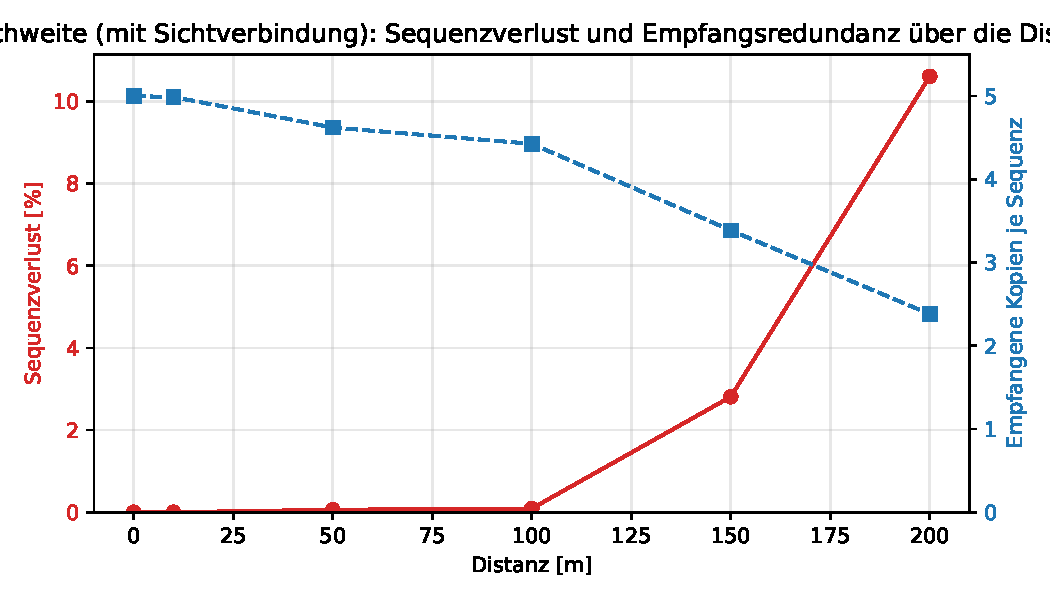
\includegraphics[width=\linewidth]{../test_programs/results/analysis/figures/range_distance.pdf}
  \caption{Sequenzverlust und Empfangsredundanz in Abhängigkeit der Distanz bei
    freier Sichtverbindung. Die Redundanz nimmt bereits ab, während der
    Sequenzverlust noch nahezu bei null liegt.}
  \label{fig:range-distanz}
\end{figure}

Bis einschließlich 100\,m ist die Übertragung praktisch verlustfrei: Bei 50\,m
gingen 7 von 11\,992 Sequenzwerten verloren (0,06\,\%), bei 100\,m 11 von 11\,992
(0,09\,\%). Die längste zusammenhängende Verlustserie beträgt dabei 25\,ms
respektive 75\,ms, und der Anteil der Sekundenfenster mit einer für die
Bewegungswahrnehmung relevanten Verlustserie liegt bei 0\,\% respektive
0,33\,\%. In diesem Bereich ist die Funkstrecke für die Lichtausgabe damit
unauffällig.

Zwischen 100\,m und 150\,m tritt ein deutlicher Übergang auf. Der Sequenzverlust
steigt auf 2,81\,\%, der Anteil vollständig verlustfreier Sekundenfenster fällt
von 97,0\,\% auf 61,0\,\%, und in 8,67\,\% der Fenster wird die Standzeit um
mindestens 50\,ms verlängert. Ebenso deutlich zeigt sich der Übergang am
95.~Perzentil des fensterbezogenen Verlusts: Bis 100\,m liegt es bei 0\,\%, bei
150\,m bereits bei 12,22\,\%. Bei 200\,m liegt der Verlust bei 10,61\,\%, nur
noch 8,67\,\% der Fenster sind verlustfrei, 40,67\,\% enthalten eine sichtbar
relevante Verlustserie, das 95.~Perzentil erreicht 31,72\,\% und die längste
Verlängerung der Standzeit 425\,ms. Der mittlere Abstand empfangener
Sequenzwerte wächst dabei von 25,0\,ms auf 28,5\,ms die effektive
Aktualisierungsrate sinkt damit von 40\,Hz auf rund 35\,Hz. Der gleichzeitige
Anstieg des Jitters von 6,6\,ms auf 14,9\,ms ist dabei keine unabhängige
Beobachtung, sondern ergibt sich aus den Verlustlücken selbst
(Abschnitt~\ref{subsec:metriken}).

Anders als der Verlust verläuft die Empfangsredundanz über die gesamte Messreihe
streng monoton: 5,00 (0\,m), 4,99 (10\,m), 4,62 (50\,m), 4,43 (100\,m), 3,39
(150\,m) und 2,38 Kopien je Sequenzwert bei 200\,m. Sie ist damit die
aussagekräftigere Größe zur Bewertung der Reichweite, denn sie zeigt den Rückgang
der Fehlerreserve bereits an, während der Sequenzverlust noch nahezu bei null
liegt.
Zugleich erklärt sie den flachen Verlauf des Verlusts bis 100\,m: Solange
mindestens eine der fünf Kopien eintrifft, bleibt der Sequenzwert vollständig
erhalten. Erst wenn die Redundanz gegen eins sinkt, schlägt jede weitere
Verschlechterung unmittelbar auf die Lichtausgabe durch.

Die zeitliche Auflösung der Läufe in Abbildung~\ref{fig:range-zeit} zeigt, dass
die Verluste bei den großen Distanzen nicht auf einzelne Störereignisse
zurückgehen, sondern über den gesamten Lauf verteilt auftreten: Im Lauf über
200\,m liegt der minutenweise gemittelte Verlust zwischen 6,41\,\% und 16,40\,\%,
im Lauf über 150\,m zwischen 2,14\,\% und 3,61\,\%. Maßgeblich für das
Verlustniveau ist damit die mit der Distanz abnehmende Reserve der Strecke und
nicht eine kurzzeitige Abschattung durch Passanten oder Fahrzeuge. Die
verbleibende Schwankung zwischen den Minuten
ist mit einem Faktor von 2,6 im 200-m-Lauf allerdings erheblich und zeigt, dass
die Umgebung auch bei freier Sicht zeitveränderlich auf die Verbindung wirkt.

Dazu passt ein Nebenbefund: Für den Lauf über 200\,m weist die Aufzeichnung einen
mittleren Fremdpegel von $-63{,}4$\,dBm aus, gegenüber rund $-80$\,dBm an allen
übrigen Messpunkten. Da dieser Wert die Aktivität fremder Sender auf dem Kanal
beschreibt und nicht den Pegel der Nutzstrecke
(Abschnitt~\ref{subsec:messgrenzen}), deutet er auf eine erhöhte Kanalbelegung
während dieses Laufs hin. Deren Beitrag lässt sich vom Einfluss der Distanz nicht
trennen.

\begin{figure}[htbp]
  \centering
  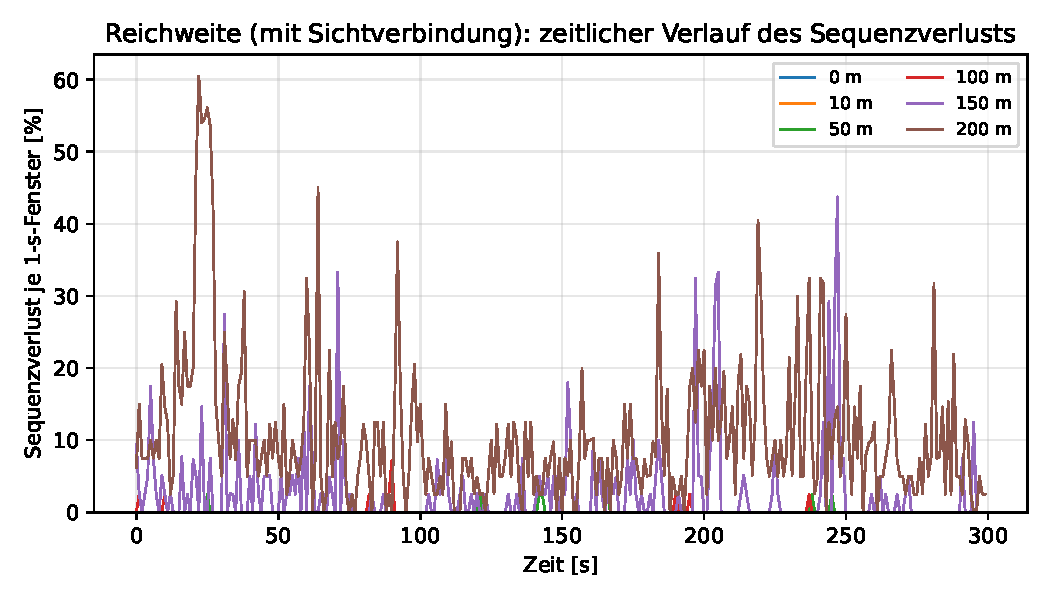
\includegraphics[width=\linewidth]{../test_programs/results/analysis/figures/range_timeseries.pdf}
  \caption{Zeitlicher Verlauf des Sequenzverlusts je Messpunkt bei freier
    Sichtverbindung. Bei 150\,m und 200\,m verteilen sich die Verluste über den
    gesamten Lauf.}
  \label{fig:range-zeit}
\end{figure}

\subsection{Messreihe ohne Sichtverbindung}
\label{subsec:reichweite-verdeckt}

Tabelle~\ref{tab:range-hidden-summary} und Abbildung~\ref{fig:range-hidden-distanz}
zeigen dieselbe Auswertung für den vollständig verdeckten Empfänger.

% Requires \usepackage{booktabs}; otherwise replace \toprule etc. with \hline.
\begin{table}[htbp]
  \centering
  \small
  \begin{tabular}{lrrrrrrr}
    \toprule
    Messpunkt & Verlust & Fenster p95 & Kopien & Jitter & max. Ausfall & Fenster & RSSI \\
    & [\%] & [\%] & je Seq. & [ms] & [ms] & ab 50 ms [\%] & [dBm] \\
    \midrule
    10 m & 0,48 & 0 & 4,80 & 6,96 & 75 & 1,67 & $-$81,23 \\
    50 m & 2,08 & 10,08 & 3,57 & 9,23 & 225 & 7,33 & $-$77,85 \\
    100 m & 10,86 & 36,64 & 2,72 & 16,45 & 575 & 37 & $-$82,97 \\
    150 m & 27,18 & 60,80 & 1,87 & 26,59 & 700 & 80 & $-$48,70 \\
    200 m & 36,29 & 63,67 & 1,61 & 32,12 & 950 & 95,67 & $-$77,39 \\
    \bottomrule
\end{tabular}
\caption{Reichweitenmessung (ohne Sichtverbindung)}
  \label{tab:range-hidden-summary}
\end{table}


\begin{figure}[htbp]
  \centering
  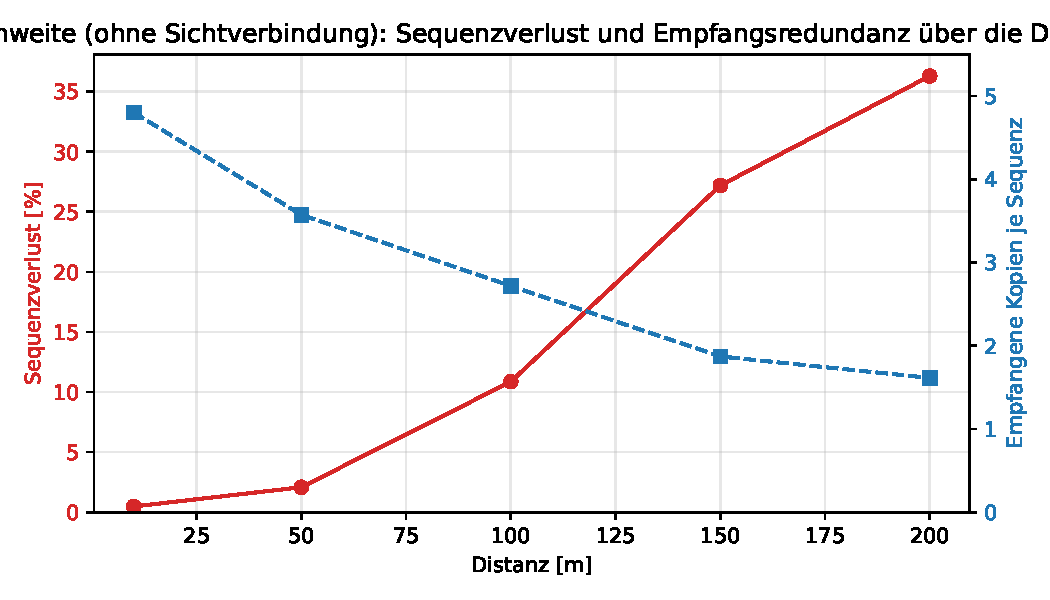
\includegraphics[width=\linewidth]{../test_programs/results/analysis/figures/range_hidden_distance.pdf}
  \caption{Sequenzverlust und Empfangsredundanz über der Distanz bei verdecktem
    Empfänger (rund 50\,cm hinter einer 1\,m breiten Stahlbetonstütze).}
  \label{fig:range-hidden-distanz}
\end{figure}

Bei 10\,m bleibt die Verbindung nahezu unbeeinträchtigt: Der Sequenzverlust
beträgt 0,48\,\%, die Redundanz 4,80 Kopien je Sequenzwert. Die Verluste sind
zudem auf ein einzelnes Ereignis in der dritten Minute konzentriert ein
Sekundenfenster weist 30,91\,\% Verlust auf, während 97,67\,\% aller Fenster
vollständig verlustfrei sind. Auf kurzer Distanz genügt die Beugung um die Stütze
also, um die Strecke zu tragen.

Mit zunehmender Entfernung verschlechtert sich die Verbindung deutlich schneller
als in der Sichtreihe. Bei 50\,m liegt der Verlust bei 2,08\,\% und die Redundanz
bei 3,57. 7,33\,\% der Sekundenfenster enthalten eine Verlustserie ab 50\,ms, die
längste Verlängerung der Standzeit beträgt 225\,ms. Bei 100\,m steigt der Verlust
auf 10,86\,\%, die Redundanz fällt auf 2,72, und in 37,00\,\% der Fenster wird die
Wahrnehmungsschwelle überschritten. Bei 150\,m gehen bereits 27,18\,\% der
Sequenzwerte verloren, die Redundanz beträgt noch 1,87 Kopien, 80,00\,\% der
Fenster überschreiten die Schwelle und lediglich 0,67\,\% zwei von 300
sind vollständig verlustfrei. Bei 200\,m schließlich ist die Strecke nicht
mehr sinnvoll nutzbar: 36,29\,\% der Sequenzwerte gehen verloren, die Redundanz
sinkt auf 1,61 Kopien in einzelnen Fenstern auf exakt 1,00, \emph{kein
einziges} Sekundenfenster ist verlustfrei, 95,67\,\% der Fenster überschreiten
die 50-ms-Schwelle und die längste Verlängerung der Standzeit erreicht 950\,ms.
Der mittlere Abstand empfangener Sequenzwerte wächst auf 42,3\,ms, was einer
effektiven Aktualisierungsrate von rund 24\,Hz entspricht. Die Übertragung
unterschreitet damit erstmals die in Abschnitt~\ref{subsec:echtzeitverhalten}
angestrebte Aktualisierungsrate.

Auch hier zeigt die zeitliche Auflösung (Abbildung~\ref{fig:range-hidden-zeit})
eine zusätzliche Variabilität der Umgebung: Im Lauf über 100\,m liegt der Verlust
in den ersten drei Minuten zwischen 12,63\,\% und 19,08\,\%, in den letzten
beiden dagegen nur bei 2,51\,\% und 3,91\,\%. Eine kontrollierte Zuordnung zu
konkreten Umgebungsereignissen ist aus den Daten nicht möglich. Die Beobachtung
belegt jedoch, dass auf verdeckten Strecken neben der Distanz auch
zeitveränderliche Einflüsse eine erhebliche Rolle spielen. Der Lauf über 150\,m
zeigt umgekehrt keinen solchen Verlauf: Sein minutenweiser Verlust bleibt
durchgehend zwischen 22,58\,\% und 29,19\,\%, die Strecke ist über die gesamte
Messdauer gleichmäßig schlecht. Für diesen Messpunkt weist die Aufzeichnung
allerdings einen mittleren Fremdpegel von $-48{,}7$\,dBm aus und damit den
höchsten Wert aller Läufe. Wie beim 200-m-Lauf der Sichtreihe ist eine erhöhte
Kanalbelegung als zusätzlicher Einfluss nicht auszuschließen
(Abschnitt~\ref{subsec:messgrenzen}).

\begin{figure}[htbp]
  \centering
  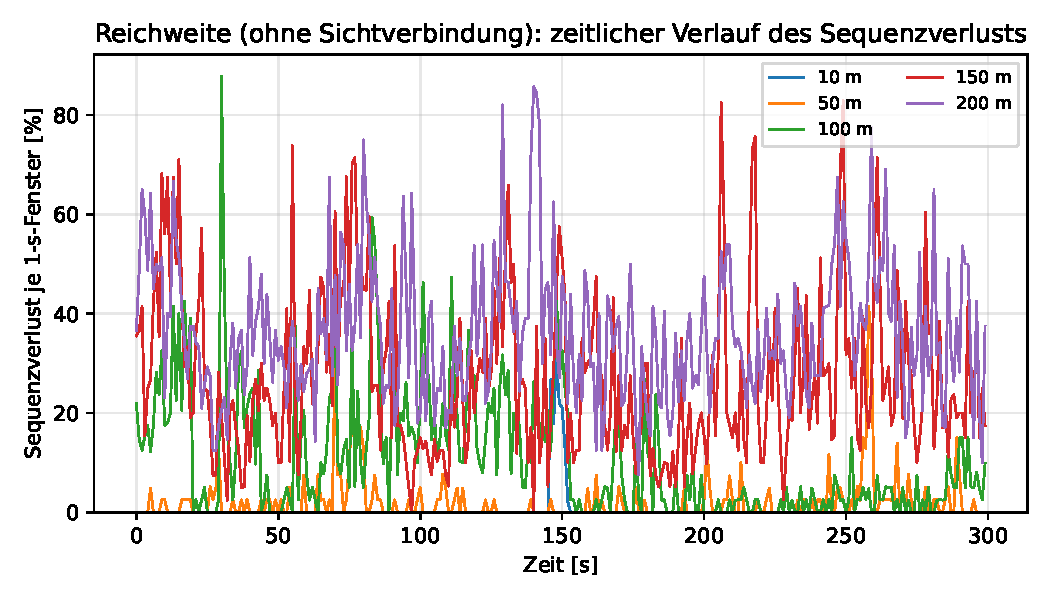
\includegraphics[width=\linewidth]{../test_programs/results/analysis/figures/range_hidden_timeseries.pdf}
  \caption{Zeitlicher Verlauf des Sequenzverlusts je Messpunkt bei verdecktem
    Empfänger. Der Lauf über 100\,m verbessert sich in der zweiten Hälfte
    deutlich.}
  \label{fig:range-hidden-zeit}
\end{figure}

\subsection{Vergleich und Bewertung}
\label{subsec:reichweite-bewertung}

Der Vergleich beider Reihen bei gleicher Distanz quantifiziert die Wirkung der
Abschattung. Bei 50\,m steigt der Verlust von 0,06\,\% auf 2,08\,\% und die
Redundanz sinkt von 4,62 auf 3,57 Kopien. Bei 100\,m stehen 0,09\,\% und 4,43
Kopien einem Verlust von 10,86\,\% bei 2,72 Kopien gegenüber. Das verdeckte
Verhalten bei 100\,m entspricht dabei praktisch dem Verhalten der Sichtreihe bei
200\,m (10,61\,\%, 2,38 Kopien).

Die Abschattung wirkt wie ein näherungsweise konstanter Dämpfungszuschlag. Da ein
solcher Zuschlag im logarithmischen Pfadverlustmodell einem konstanten Faktor der
Distanz entspricht, lässt sich die Wirkung als äquivalente Sichtdistanz
ausdrücken. Vergleicht man die verdeckten Messpunkte anhand der Empfangsredundanz
mit der interpolierten Sichtreihe, ergeben sich Faktoren von etwa 2,8 bei 50\,m,
1,8 bei 100\,m und 1,5 bei 150\,m. Als Faustregel lässt sich daraus ableiten,
dass die vollständige Abschattung durch eine Stahlbetonstütze etwa die Hälfte der
nutzbaren Distanz kostet. Angesichts eines einzelnen Laufs je Messpunkt und der
Streuung zwischen den ermittelten Faktoren ist dieser Wert als Größenordnung und
nicht als belastbarer Zahlenwert zu verstehen.

Für die praktische Bewertung ist die in Abschnitt~\ref{subsec:fa-kommunikation}
festgelegte Mindestreichweite von 50\,m maßgeblich. Mit Sichtverbindung wird
diese Anforderung deutlich übertroffen: Bei 50\,m ist die Übertragung mit
0,06\,\% Verlust und ohne ein einziges kritisches Sekundenfenster faktisch
fehlerfrei, und auch bei 100\,m bleibt dieses Niveau erhalten. Ohne
Sichtverbindung wird die Mindestreichweite ebenfalls erreicht, jedoch mit
sichtbar geringerer Reserve: Bei 2,08\,\% Verlust und 7,33\,\% kritischen Fenstern
ist im Mittel etwa alle 14\,s mit einer verlängerten Standzeit von mindestens
50\,ms zu rechnen. Für die Betriebsplanung folgt daraus die Empfehlung, mit
Sichtverbindung bis etwa 100\,m und ohne Sichtverbindung bis etwa 50\,m zu
projektieren. Jenseits von 150\,m (Sicht) beziehungsweise 100\,m (verdeckt) ist
der Betrieb zwar noch möglich, aber nicht mehr zuverlässig planbar.

\section{Verhalten in hochfrequenzbelasteter Umgebung}
\label{sec:stoerfestigkeit}

Zur Beurteilung der Störfestigkeit wurden zwei Läufe im Lesesaal einer Bibliothek
aufgezeichnet. Sender und Empfänger standen dabei rund 50\,m voneinander
entfernt, wobei die direkte Sichtlinie durch hölzernes Mobiliar unterbrochen war.
Die Messung fand damit genau an der in Abschnitt~\ref{subsec:fa-kommunikation}
geforderten Mindestreichweite statt. Positionen von Sender und Empfänger,
Abstand, Kanal und Firmwarestand blieben zwischen beiden Läufen unverändert
verändert wurde
ausschließlich die Umgebung: Der erste Lauf fand zur Stoßzeit bei hoher
Personendichte und entsprechend vielen aktiven WLAN- und Bluetooth-Geräten statt,
der zweite zur Nebenzeit bei nahezu leerem Lesesaal. Es handelt sich damit um eine
Feldmessung mit realistischer, aber nicht kontrollierter Störlast.
Tabelle~\ref{tab:interference-summary} zeigt die Ergebnisse,
Abbildung~\ref{fig:stoerung-zeit} den zeitlichen Verlauf.

% Requires \usepackage{booktabs}; otherwise replace \toprule etc. with \hline.
\begin{table}[htbp]
  \centering
  \small
  \begin{tabular}{lrrrrrrr}
    \toprule
    Szenario & Verlust & Fenster p95 & Kopien & Jitter & max. Ausfall & Fenster & RSSI \\
    & [\%] & [\%] & je Seq. & [ms] & [ms] & ab 50 ms [\%] & [dBm] \\
    \midrule
    Nebenzeit & 0,01 & 0 & 4,57 & 6,47 & 25 & 0 & $-$83,72 \\
    Stoßzeit & 0,51 & 2,50 & 3,83 & 8,45 & 750 & 0,33 & $-$84,02 \\
    \bottomrule
\end{tabular}
\caption{Messergebnisse Störfestigkeit}
  \label{tab:interference-summary}
\end{table}


\begin{figure}[htbp]
  \centering
  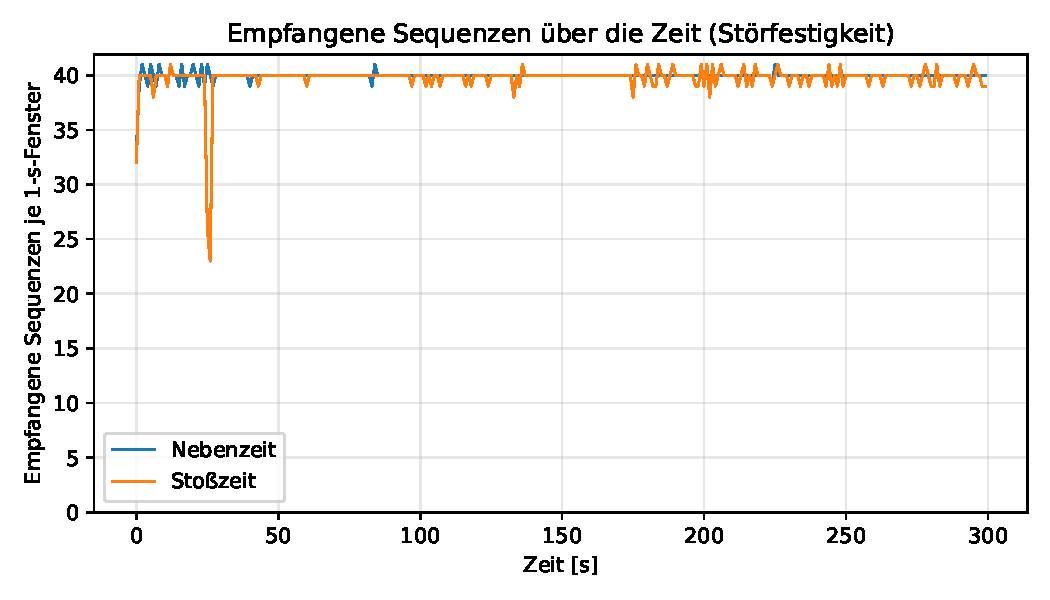
\includegraphics[width=\linewidth]{../test_programs/results/analysis/figures/interference_timeseries.pdf}
  \caption{Empfangene Sequenzen je Sekunde zur Stoßzeit und zur Nebenzeit. Der
    Sollwert beträgt 40 Sequenzen je Sekunde.}
  \label{fig:stoerung-zeit}
\end{figure}

Zur Nebenzeit ist die Übertragung nahezu fehlerfrei: Ein einziger von 11\,992
Sequenzwerten geht verloren (0,01\,\%), 99,67\,\% der Sekundenfenster sind
vollständig verlustfrei und die längste Verlängerung der Standzeit beträgt
25\,ms. Zur Stoßzeit
steigt der Sequenzverlust auf 0,51\,\% (61 von 11\,991), der Anteil verlustfreier
Fenster sinkt auf 89,67\,\% und der Jitter wächst von 6,5\,ms auf 8,5\,ms. Die
Empfangsredundanz geht von 4,57 auf 3,83 Kopien je Sequenzwert zurück. Die
Fehlerreserve der Strecke verringert sich also messbar, bleibt aber mit fast vier
von fünf Kopien komfortabel erhalten.

Der Wert zur Nebenzeit ordnet zugleich den Aufbau ein: Mit 4,57 Kopien liegt er
praktisch auf dem Niveau der freien 50-m-Strecke des Reichweitentests (4,62) und
deutlich über der dort vollständig verdeckten Strecke gleicher Länge (3,57). Die
hölzerne Möblierung kostet also kaum Reserve. Der Rückgang zur Stoßzeit ist damit
der veränderten Kanalauslastung zuzuordnen und nicht dem Abstand oder der
Abschattung.

Praktisch bedeutsamer als die mittlere Verlustrate ist die Struktur der Verluste.
Der überwiegende Teil des Unterschieds geht auf ein einzelnes Ereignis in der
ersten Minute des Stoßzeitlaufs zurück: Dort fielen 30 aufeinanderfolgende
Sequenzwerte aus, was die Standzeit um 750\,ms verlängert. Das betroffene
Sekundenfenster weist 56,60\,\% Verlust auf. In allen übrigen Fenstern beträgt die
längste Verlustserie einen einzigen Sequenzwert (25\,ms), sodass insgesamt nur
0,33\,\% der Fenster die Wahrnehmungsschwelle überschreiten. Eine Unterbrechung
von 750\,ms ist im laufenden Betrieb als eingefrorener Lichtzustand deutlich
sichtbar die Störfestigkeit ist damit nicht durch die mittlere Rate, sondern
durch die Häufigkeit solcher Einzelereignisse begrenzt.

Der mittlere Fremdpegel auf dem Kanal fällt in beiden Läufen praktisch identisch
aus: $-84{,}0$\,dBm zur Stoßzeit und $-83{,}7$\,dBm zur Nebenzeit. Die veränderte
Kanalauslastung schlägt sich in diesem Hilfsmaß somit nicht nieder, was die in
Abschnitt~\ref{subsec:messgrenzen} beschriebene eingeschränkte Aussagekraft der
RSSI-Erfassung bestätigt. Als Erklärung des gemessenen Effekts liegt die
Konkurrenz um den Kanal am nächsten: ESP-NOW nutzt denselben CSMA/CA-Zugriff wie
WLAN (Abschnitt~\ref{subsec:24ghz-medienzugriff}), sodass bei hoher
Kanalauslastung Sendeversuche verzögert oder verworfen werden. Dazu passen der
gleichzeitige Anstieg des Jitters und der Rückgang der Redundanz bei
unveränderter Geometrie. Ein unmittelbarer Nachweis ist mit dem verwendeten
Aufbau jedoch nicht möglich, da der Sender nicht protokolliert, ob ein Paket
abgesetzt werden konnte, und der Empfänger ein nicht gesendetes Paket nicht von
einem auf der Strecke verlorenen unterscheiden kann
(Abschnitt~\ref{subsec:messgrenzen}).

\section{Elektrische Leistungsaufnahme}
\label{sec:leistungsaufnahme}

Die elektrische Auslegung des Systems geht von einer maximalen Leistungsaufnahme
von 24\,W und einem daraus folgenden Betriebsstrom von 2\,A je Leuchtröhre aus
(Abschnitt~\ref{subsec:elektrische-belastbarkeit}). Dieser Wert ist aus dem
Datenblatt des LED-Strips gerechnet. Zur Überprüfung wurde die tatsächliche
Leistungsaufnahme einer vollständig aufgebauten Leuchtröhre gemessen.

Die Messergebnisse sind im Anhang~\ref{sec:anhang-leistungsaufnahme} dokumentiert.

Gemessen wurde netzseitig mit einem Steckdosenmessgerät vor dem Netzteil
(12\,V, 10\,A). Die Verluste des Netzteils sind in allen Werten somit enthalten.
Die vermessene Röhre entspricht mit 2\,m Länge und 120~Pixeln der Auslegung aus
Abschnitt~\ref{subsec:elektrische-belastbarkeit}. Tabelle~\ref{tab:leistung}
zeigt die drei aufgenommenen Betriebszustände.

\begin{table}[htbp]
  \centering
  \small
  \begin{tabular}{lr}
    \toprule
    Betriebszustand & Leistungsaufnahme \\
    \midrule
    Netzteil ohne angeschlossene Röhre & 0,2\,W \\
    Röhre angeschlossen, LEDs ausgeschaltet & 5,1\,W \\
    Alle Farbkanäle dauerhaft auf Maximum & 18,7\,W \\
    \bottomrule
  \end{tabular}
  \caption{Netzseitig gemessene Leistungsaufnahme einer Leuchtröhre einschließlich
    Netzteil.}
  \label{tab:leistung}
\end{table}

Für die Bewertung ist entscheidend, dass die netzseitige Messung eine obere
Schranke der Aufnahme auf der 12-V-Seite darstellt, da sie die Verluste des
Netzteils einschließt. Selbst unter der Annahme eines verlustfreien Netzteils
folgt aus den gemessenen 18,7\,W ein Betriebsstrom von höchstens
$18{,}7\,\text{W} / 12\,\text{V} \approx 1{,}56\,\text{A}$. Bei einem
realistischen Wirkungsgrad von 85\,\% sind es rund 1,3\,A. Der ausgelegte
Betriebsstrom von 2\,A wird damit eingehalten, und zwar unabhängig davon, welcher
Wirkungsgrad für das Netzteil angesetzt wird.

Zugleich erweist sich der rechnerische Ansatz als konservativ: Den 24\,W auf der
Gleichspannungsseite stehen 18,7\,W netzseitig gegenüber, obwohl darin die
Verluste des Netzteils noch enthalten sind. Der Datenblattwert von 0,2\,W je
Pixel beschreibt demnach einen Grenzwert, der auch bei voller Aussteuerung aller
drei Farbkanäle nicht ausgeschöpft wird. Die in
Abschnitt~\ref{subsec:elektrische-belastbarkeit} geforderte Auslegung mit Reserve
ist damit nicht nur gerechnet, sondern gemessen.

Bemerkenswert ist der mittlere Betriebszustand. Bereits mit ausgeschalteten LEDs
nimmt die Röhre 5,1\,W auf, abzüglich der Leerlaufaufnahme des Netzteils also
rund 4,9\,W und damit gut ein Viertel ihrer Volllastaufnahme. Dieser Anteil
entfällt auf den Mikrocontroller, das Display und den Ruhestrom der 120
Controller-Bausteine des LED-Strips, die auch bei dunklem Pixel aus der
12-V-Versorgung gespeist werden (Abschnitt~\ref{subsec:leistung-led}). Für die
Planung größerer Installationen ist dieser Sockel relevant: Zwanzig Röhren nehmen
bereits im dunklen Zustand rund 100\,W auf.

Der gemessene Betriebsstrom bleibt damit in allen Betriebszuständen innerhalb der
Auslegung der stromführenden Komponenten
(Abschnitt~\ref{subsec:elektrische-belastbarkeit}), die ihrerseits mit Reserve
gegenüber dem rechnerischen Wert dimensioniert sind
(Abschnitt~\ref{subsec:pcb-fertigung}).

\section{Bewertung gegenüber den Anforderungen}
\label{sec:anforderungsabgleich}

Tabelle~\ref{tab:anforderungsabgleich} stellt die gemessenen Kenngrößen den
Anforderungen aus Kapitel~\ref{chap:anforderungsanalyse} gegenüber.

\begin{table}[htbp]
  \centering
  \small
  \begin{tabular}{lll}
    \toprule
    Anforderung & Messergebnis & Bewertung \\
    \midrule
    Aktualisierungsrate $\geq$ 24\,Hz & 25,00\,ms mittlerer Sequenzabstand & erfüllt \\
    Jitter unterhalb Wahrnehmung & 4,1--6,6\,ms bis 100\,m & erfüllt \\
    Zuverlässigkeit ohne Störer & 0 von 23\,984 Sequenzen verloren & erfüllt \\
    Mindestreichweite 50\,m (Sicht) & 0,06\,\% Verlust, kein kritisches Fenster & erfüllt \\
    Mindestreichweite 50\,m (verdeckt) & 2,08\,\% Verlust, 7,33\,\% kritische Fenster & eingeschränkt \\
    Stabilität bei Fremdfunklast & 0,51\,\% Verlust, ein Ausfall von 750\,ms & erfüllt \\
    Definiertes Verhalten bei Ausfall & Halten des letzten Zustands & erfüllt \\
    Betriebsstrom höchstens 2\,A & 18,7\,W netzseitig, $\leq$ 1,56\,A bei 12\,V & erfüllt \\
    Ausbaugröße 20 Röhren & 8 Röhren gleichzeitig betrieben & eingeschränkt \\
    Gleichzeitige Ausgabe an allen Röhren & kein Versatz bei 120\,fps ($<4{,}2$\,ms) & erfüllt \\
    Betriebsmodi Standalone, Master, DMX & funktional verifiziert & erfüllt \\
    Signaleingänge DMX und Art-Net & funktional verifiziert & erfüllt \\
    Persistenz der Konfiguration & nach Neustart wiederhergestellt & erfüllt \\
    \midrule
    \multicolumn{3}{l}{\emph{Über die Anforderung hinaus untersucht}} \\
    Betrieb bis 200\,m (Sicht) & 10,61\,\% Verlust, Redundanz 2,38 & bedingt nutzbar \\
    Betrieb bis 100\,m (verdeckt) & 10,86\,\% Verlust, Redundanz 2,72 & bedingt nutzbar \\
    Betrieb bis 200\,m (verdeckt) & 36,29\,\% Verlust, Redundanz 1,61 & nicht nutzbar \\
    \bottomrule
  \end{tabular}
  \caption{Abgleich der Messergebnisse mit den Anforderungen aus
    Kapitel~\ref{chap:anforderungsanalyse}.}
  \label{tab:anforderungsabgleich}
\end{table}

Die Anforderungen an Echtzeitverhalten, Reichweite, Zuverlässigkeit und
elektrische Belastbarkeit werden im geforderten Einsatzbereich erfüllt, im Fall
der Reichweite mit freier Sicht sogar deutlich übertroffen. Zwei Punkte bleiben
eingeschränkt: die verdeckte Strecke an der Mindestreichweite, die mit 2,08\,\%
Verlust nutzbar bleibt, aber wenig Reserve besitzt, sowie die Ausbaugröße, von
der acht der geforderten zwanzig Röhren tatsächlich gemeinsam betrieben wurden.
Die übrigen Einschränkungen betreffen ausschließlich Bereiche jenseits der
Anforderung: große Distanzen und vollständig verdeckte Strecken.
Da sich die Empfangsredundanz in beiden Messreihen als der Mechanismus erweist,
der Einzelverluste abfängt, ist sie zugleich der Ansatzpunkt für Verbesserungen:
Eine bedarfsgerechte Erhöhung der Wiederholrate oder ein automatischer
Kanalwechsel bei einbrechender Redundanz würden genau an der Größe ansetzen, die
in allen Messreihen als früher Indikator einer sich verschlechternden Verbindung
auftritt sie sinkt bereits messbar, während der Sequenzverlust noch nahezu bei
null liegt. Diese Möglichkeiten werden in Kapitel~\ref{chap:diskussion-und-ausblick}
aufgegriffen.

\section{Grenzen der Untersuchung}
\label{sec:grenzen}

Die erhobenen Daten decken nicht alle Aspekte ab, die für eine abschließende
Bewertung des Systems erforderlich wären. Die folgenden Einschränkungen sind bei
der Interpretation der Ergebnisse zu berücksichtigen:

\begin{itemize}
  \item Je Messpunkt wurde ein Lauf aufgezeichnet. Streuungen zwischen
    Wiederholungen desselben Messpunkts sind damit nicht quantifizierbar, obwohl
    die zeitliche Struktur einzelner Läufe zeigt, dass sie erheblich sein können.
  \item Sämtliche Messreihen wurden mit einer einzelnen empfangenden Leuchtröhre
    aufgezeichnet. Der funktionale Betrieb wurde zwar mit acht gleichzeitig
    angesteuerten Röhren erprobt (Abschnitt~\ref{sec:funktionale-tests}), die
    geforderte Ausbaugröße von zwanzig Röhren jedoch weder funktional noch
    messtechnisch überprüft. Dass zusätzliche Empfänger die Funkstrecke nicht
    zusätzlich belasten, folgt aus der Broadcast-Topologie, ist aber nicht
    gemessen.
  \item Die Leistungsmessung umfasst je Betriebszustand einen Messwert an einer
    einzelnen Röhre. Die Messunsicherheit des verwendeten Steckdosenmessgeräts
    ist nicht quantifiziert, und die Aufteilung der Aufnahme zwischen LED-Strip
    und Steuerelektronik wurde nicht getrennt erfasst. Der ausgewiesene
    Leerlaufwert des Netzteils von 0,2\,W liegt an der Auflösungsgrenze solcher
    Geräte.
  \item Die verdeckte Messreihe untersucht mit der Stahlbetonstütze genau eine
    Hindernisgeometrie. Andere Materialien, Wandstärken und Abstände zwischen
    Empfänger und Hindernis können zu deutlich abweichenden Ergebnissen führen.
    Die abgeleitete Faustregel ist daher nicht verallgemeinerbar.
  \item Die Störlast der Bibliotheksmessung war realistisch, aber weder
    kontrolliert noch unabhängig quantifiziert und erreicht nicht das Niveau
    einer Veranstaltung. Ein reproduzierbarer Laborversuch mit definierten
    Störern sowie eine Messung nach Kanalwechsel stehen aus.
  \item Die RSSI-Erfassung ist aus den in Abschnitt~\ref{subsec:messgrenzen}
    genannten Gründen nicht als Pfadverlustmessung verwertbar.
\end{itemize}

\chapter{Diskussion und Ausblick}
\label{chap:diskussion-und-ausblick}

\section{Diskussion der Ergebnisse}
\label{sec:diskussion-der-ergebnisse}

\subsection{Redundanz statt Quittierung}
\label{subsec:diskussion-redundanz}

Die zentrale Entwurfsentscheidung der Funkstrecke besteht darin, auf einen
Rückkanal zu verzichten und die fehlende Zustellgarantie stattdessen durch
mehrfache Aussendung desselben Datenstands zu kompensieren
(Abschnitt~\ref{subsec:drahtlose-uebertragung}). Diese Entscheidung war zum
Zeitpunkt des Entwurfs eine Annahme: die Messungen belegen nun ihre
Tragfähigkeit. Über eine Distanz von 100\,m mit Sichtverbindung bleibt der
Sequenzverlust bei 0,09\,\%, obwohl die Empfangsredundanz zu diesem Zeitpunkt
bereits von fünf auf 4,43 Kopien je Sequenzwert gesunken ist. Die Strecke
verliert also messbar an Qualität, ohne dass sich dies auf die Lichtausgabe
auswirkt, genau dies ist die Funktion, die der Redundanz zugedacht war.

Aus dieser Beobachtung folgt ein Gedanke, der über die Bewertung der einzelnen
Messreihe hinausreicht. Die Empfangsredundanz ist eine Zustandsgröße der
Funkstrecke, die ohne Rückkanal allein empfängerseitig bestimmbar ist. Die
Röhre kann zählen, wie viele Kopien eines Sequenzwerts sie erhalten hat, und
daraus auf die verbleibende Fehlerreserve schließen. Ein unidirektional
ausgelegtes System kann seinen eigenen Verbindungszustand somit kennen, ohne die
in Abschnitt~\ref{sec:abgrenzung} bewusst ausgeschlossene bidirektionale
Kommunikation einzuführen. Diese Eigenschaft ist die Voraussetzung für jede Form
der Selbstanpassung und wird in Abschnitt~\ref{subsec:ausblick-messungen} wieder
aufgegriffen.

Die Messungen erlauben darüber hinaus eine genauere Bestimmung dessen, wogegen
die Redundanz überhaupt schützt. Die fünf Kopien eines Sequenzwerts werden
innerhalb desselben 25-ms-Fensters ausgesendet
(Abschnitt~\ref{subsec:messaufbau}). Die Redundanz ist damit eine rein zeitliche
Wiederholung innerhalb eines sehr kurzen Intervalls. Sie wirkt folglich gegen
unkorrelierte Einzelverluste eine Kollision, eine kurzzeitige
Kanalbelegung, ein einzelnes gestörtes Paket, weil in diesen Fällen mindestens
eine der übrigen Kopien den Empfänger erreicht. Gegen korrelierte Störungen,
die länger als 25\,ms andauern, ist sie hingegen wirkungslos: Überschreitet die
Störung dieses Fenster, gehen alle fünf Kopien desselben Werts gemeinsam verloren.

Genau dieses Verhalten belegen beide Messreihen. Die Unterbrechung von 750\,ms im
Stoßzeitlauf umfasst 30 aufeinanderfolgende Sequenzwerte und damit 150 einzeln
ausgesendete Pakete. Ebenso wachsen mit zunehmender Distanz nicht nur die
Verlustraten, sondern vor allem die Längen der zusammenhängenden Verlustserien.
Der praktisch relevante Fehlerfall ist somit nicht der Einzelverlust, gegen den
das Verfahren ausgelegt ist, sondern der zeitlich ausgedehnte Ausfall. Daraus
folgt eine Einschränkung für jede Weiterentwicklung des Ansatzes: Eine bloße
Erhöhung der Kopienzahl innerhalb desselben Fensters verbessert die Robustheit
gegenüber solchen Ereignissen nicht.

Ebenso deutlich zeigen die Messungen die Grenze des Prinzips. Der Sequenzverlust
wächst nicht proportional zur Verschlechterung der Strecke, sondern bleibt lange
nahezu unverändert und springt anschließend sprunghaft an, sobald die Redundanz
gegen eins geht. Im verdeckten Lauf über 200\,m stehen im Mittel noch 1,61 Kopien
je Sequenzwert zur Verfügung, in einzelnen Fenstern genau eine und der Verlust
erreicht 36,29\,\%. Das Verfahren puffert also über einen weiten Bereich sehr
wirkungsvoll und versagt dann innerhalb einer kurzen Spanne. Für die Praxis
bedeutet dies, dass ein System, das nur den Sequenzverlust beobachtet, keine
Vorwarnzeit besitzt: Bis kurz vor dem Zusammenbruch der Verbindung erscheint die
Übertragung fehlerfrei.

\subsection{Broadcast ohne Rückkanal}
\label{subsec:diskussion-broadcast}

Der Verzicht auf Quittierung ist Teil einer umfassenderen Entscheidung für eine
verbindungslose Broadcast-Topologie. Ihr Gewinn liegt in der Einfachheit: Der
Sendeaufwand der Bridge ist unabhängig von der Anzahl der Empfänger, alle Röhren
erhalten denselben Datenstand innerhalb desselben Übertragungsfensters, und die
Adressierung erfolgt lokal am Gerät statt über ein Funkprotokoll
(Abschnitt~\ref{subsec:synchronisation-roehem}). Die Gleichzeitigkeit ist dabei
nicht nur eine Eigenschaft des Entwurfs, sondern messtechnisch bestätigt: In der
Zeitlupenaufnahme mit 120~Bildern je Sekunde wechseln acht gemeinsam betriebene
Röhren innerhalb desselben Einzelbildes
(Abschnitt~\ref{sec:gleichzeitigkeit}). Der Preis dafür ist ebenso klar:
Es existiert weder ein Zustellnachweis noch eine Möglichkeit zur Ferndiagnose. Ein
Ausfall einzelner Röhren wird nicht gemeldet, sondern erst optisch sichtbar.

Die Störfestigkeitsmessung erlaubt es, diesen Zielkonflikt genauer zu bewerten,
als es beim Entwurf möglich war. Das einzige praktisch relevante Ereignis des
Stoßzeitlaufs eine zusammenhängende Unterbrechung von 750\,ms lässt sich am
ehesten auf die Konkurrenz um den Übertragungskanal zurückführen und nicht auf
die fehlerhafte Zustellung einzelner Pakete: Sämtliche Kopien des betroffenen
Zeitabschnitts blieben aus, während Abstand und Aufbau unverändert waren
(Abschnitt~\ref{sec:stoerfestigkeit}). Ein unmittelbarer Nachweis ist mit dem
verwendeten Aufbau nicht möglich, da senderseitig nicht protokolliert wird, ob
ein Paket abgesetzt werden konnte. Unter dieser Deutung hätte ein
Quittierungsverfahren das Ereignis nicht verhindert. Es hätte den Ausfall
lediglich erkennbar gemacht und zugleich zusätzliche Sendevorgänge auf einem
bereits ausgelasteten Kanal erzeugt.
Die Entscheidung gegen den Rückkanal wird durch die Messung also nicht relativiert,
sondern gestützt allerdings mit der Einschränkung, dass die fehlende
Rückmeldung den Betreiber im Fehlerfall ohne Information lässt.

Der Zugriff auf das Medium erfolgt nach demselben CSMA/CA-Verfahren wie
bei WLAN, sodass die verfügbare Sendezeit mit der Fremdlast auf dem gewählten
Kanal konkurriert. Die Implementierung sieht hierfür drei gespreizte Kanäle vor
(Abschnitt~\ref{subsec:espnow}), überlässt die Auswahl jedoch dem Anwender. Der
Betrieb hängt damit an einer Konfigurationsentscheidung, die vor der Veranstaltung
zu treffen ist.

\subsection{Reichweite als Eigenschaft des Aufbaus}
\label{subsec:diskussion-abschattung}

Der aufschlussreichste Befund der Reichweitenmessung ist nicht die erreichte
Maximaldistanz, sondern der Vergleich beider Messreihen. Dieselbe Hardware, derselbe
Kanal und dieselbe Sendeleistung führen zu deutlich unterschiedlichen Ergebnissen,
je nachdem, ob die Sichtlinie frei ist oder durch ein massives Bauteil unterbrochen
wird. Die verdeckte Strecke verhält sich näherungsweise wie eine etwa doppelt so
lange freie Strecke (Abschnitt~\ref{subsec:reichweite-bewertung}). Reichweite ist
demnach keine Eigenschaft des Geräts, sondern eine Eigenschaft des Aufbaus. Für die
Anwendung folgt daraus eine unmittelbar umsetzbare Konsequenz: Die Positionierung
der Bridge auf einer möglichst freien Sichtachse und in erhöhter Lage wirkt
stärker auf die Verbindungsqualität als jede Steigerung der Sendeleistung, und eine
ungünstig platzierte Bridge lässt sich durch Reserven auf der Funkstrecke nicht
ausgleichen.

Dieser Befund verbindet die Arbeit mit der in
Abschnitt~\ref{subsec:forschung-kommunikation} beschriebenen Lösung von Yang et al.
Dort werden abgeschattete Empfänger über ein Kabel an einen erreichbaren Empfänger
angebunden, also durch das Wiedereinführen genau jener Verkabelung, deren
Vermeidung das erklärte Ziel des Ansatzes war. Die vorliegende Messreihe
quantifiziert erstmals, wie groß das zugrunde liegende Problem tatsächlich ist,
und zeigt zugleich, dass es im geforderten Einsatzbereich nicht zu diesem
Rückschritt zwingt: Bei der in Abschnitt~\ref{subsec:fa-kommunikation}
festgelegten Mindestreichweite von 50\,m bleibt die Übertragung auch bei
vollständig verdecktem Empfänger mit 2,08\,\% Sequenzverlust nutzbar.

Für den Fall größerer oder ungünstigerer Strecken bieten sich Gegenmaßnahmen an,
die den kabellosen Charakter des Systems erhalten. Naheliegend ist die Verteilung
mehrerer Bridges auf ein Veranstaltungsgelände, sodass jede Röhre eine kurze,
möglichst freie Strecke zu einem Sender besitzt. Die Broadcast-Topologie steht dem
nicht entgegen, erfordert jedoch die zuweise zu unterschiedlichen Kanälen 
inerhalb eines Sendebereichs um Interferenze zu vermeiden.
Ebenso wirksam ist die Ausrichtung und
Wahl der Antennen, die im vorliegenden Aufbau als externe Bauform ausgeführt sind
(Abschnitt~\ref{subsec:funk-antenne}) und damit ohne Eingriff in die Elektronik
getauscht werden können.

\subsection{Einordnung in den Stand der Technik}
\label{subsec:diskussion-einordnung}

Die in Abschnitt~\ref{sec:luecken-stand-der-technik} formulierte Lücke betraf
weniger die drahtlose Übertragung als solche als vielmehr den Grad der
Integration: Die betrachteten Arbeiten ersetzen jeweils nur die Übertragungsstrecke
zwischen Steuergerät und Leuchtmittel, während das Leuchtmittel selbst
kabelgebunden angesteuert bleibt. Das entwickelte System vereint Funkempfang,
Energieversorgung und Pixel Ansteuerung innerhalb der Röhre. Die
funktionale Verifikation in Abschnitt~\ref{sec:funktionale-tests} belegt, dass
mehrere unabhängig adressierte Röhren allein über die Funkstrecke betrieben
werden, und die Reichweitenmessung zeigt, dass dies über praxisrelevante
Distanzen trägt. Die Signalverkabelung entfällt damit vollständig und nicht nur
abschnittsweise.

Ein zweiter Beitrag betrifft die Bewertungsgrundlage. Die Leistungsbewertung in
\cite{yang2015real} beschränkt sich auf den Nachweis der Timing-Konformität.
Reichweite, Paketverlust und Verhalten unter Fremdfunklast bleiben unbetrachtet.
Die vorliegende Arbeit erhebt genau diese Größen und macht darüber hinaus die
Struktur der Verluste sichtbar. Dass ein Lauf mit 0,51\,\% mittlerem Verlust eine
zusammenhängende Unterbrechung von 750\,ms enthalten kann, während alle übrigen
Fenster nahezu fehlerfrei sind, ist für die Lichtwahrnehmung entscheidend und
bleibt bei einer Betrachtung von Mittelwerten unsichtbar. Die in
Abschnitt~\ref{subsec:metriken} eingeführte Trennung von Sequenzverlust und
Empfangsredundanz sowie die Auswertung der Verlustserien sind insofern
übertragbar auf andere funkgestützte Lichtsteuerungen und nicht auf das hier
entwickelte System beschränkt.

Gegenüber dem kommerziellen Premiumsegment bleiben Unterschiede bestehen, die
nicht auf die Übertragung, sondern auf den Funktionsumfang der Leuchte entfallen.
Die in Abschnitt~\ref{sec:kommerzielle-led-leuchtroehren} betrachtete
\textit{Titan Tube} bietet Akkubetrieb, eine Schutzart für den Außeneinsatz sowie
eine erweiterte Farbmischung mit zusätzlichen Mint- und Amber-Dioden, die eine
Anpassung des Weißabgleichs erlaubt. Das entwickelte System bleibt demgegenüber
netzgebunden und auf eine RGB-Mischung beschränkt. Die kabelgebundene
Pixelsteuerung ist auf der Bridge-Platine bereits vorbereitet, war jedoch
ausdrücklich nicht Gegenstand dieser Arbeit
(Abschnitt~\ref{subsec:bridge-pcb}).

Ein Vergleich der Kosten ist vor diesem Hintergrund nur mit Einschränkungen
aussagekräftig, verdeutlicht aber die Größenordnung. Den in
Abschnitt~\ref{sec:kommerzielle-led-leuchtroehren} genannten Endkundenpreisen von
etwa 800\,€ je Röhre im Premiumsegment und rund 400\,€ je Röhre bei
kostengünstigeren Systemen stehen Materialkosten von etwa 62\,€ je Röhre und rund
31\,€ je Bridge gegenüber (Abschnitt~\ref{subsec:gesamtkosten}). Diese Zahlen sind
jedoch nicht unmittelbar vergleichbar: Den die Bestückung
der Platinen, der 3D-Druck der Gehäuse, der mechanische Zusammenbau sowie die
Prüfung jeder Einheit, die im Eigenbau als Arbeitszeit anfallen und bei einem
Fertigprodukt im Preis enthalten sind fehlen. in diesen Preis. Ebenso wenig enthalten sind ein
EMV- und CE-Konformitätsnachweis und Gewährleistung.
Der Vergleich belegt daher nicht, dass das System um eine Größenordnung
günstiger ist, sondern dass die Materialkosten einer solchen Leuchte
deutlich unterhalb der Marktpreise liegen und der Eigenbau damit für Anwender
erschlossen wird, für die kommerzielle Systeme wirtschaftlich nicht in Frage
kommen. Eine weitergehende wirtschaftliche Betrachtung ist entsprechend der
Abgrenzung in Abschnitt~\ref{sec:abgrenzung} nicht Gegenstand dieser Arbeit.

\subsection{Grenzen der Aussagekraft}
\label{subsec:diskussion-aussagekraft}

Die messtechnischen Einschränkungen sind in Abschnitt~\ref{sec:grenzen}
aufgeführt. Darüber hinaus ist zu berücksichtigen, wie weit die Ergebnisse
überhaupt verallgemeinert werden können.

Sämtliche Messreihen wurden mit einem Prototyp, an jeweils einem Standort und auf
einem einzigen Kanal erhoben. Insbesondere umfasst der Messaufbau nur eine
empfangende Röhre. Der funktionale Betrieb wurde zwar mit acht gleichzeitig
angesteuerten Röhren erprobt (Abschnitt~\ref{sec:funktionale-tests}) und damit
mit knapp der Hälfte der geforderten Ausbaugröße quantitativ vermessen wurde
dieser Fall jedoch nicht. Dass zusätzliche Röhren die Funkstrecke nicht
zusätzlich belasten, folgt aus der Broadcast-Topologie.

\section{Fazit}
\label{sec:fazit}

Ziel dieser Arbeit war die Entwicklung eines Beleuchtungssystems, das
DMX-Steuersignale drahtlos an mehrere LED-Leuchtröhren überträgt
(Abschnitt~\ref{sec:zielsetzung}). Dieses Ziel wurde erreicht. Das System besteht
aus einer Bridge, die Steuerdaten aus einer bestehenden Lichtinfrastruktur
entgegennimmt oder im Master-Modus selbst erzeugt, sowie aus Leuchtröhren, die
den für ihre Adresse bestimmten Abschnitt des Datenstroms extrahieren und
unmittelbar in Licht umsetzen. Beide Betriebsarten der Bridge und der autarke
Einzelbetrieb der Röhre wurden am aufgebauten System verifiziert.

Die Anforderung an das Echtzeitverhalten wird erfüllt und der Jitter bleibt im gesamten
praxisrelevanten Bereich deutlich unterhalb des Frameabstands. Unter
Idealbedingungen wurde kein einziger Sequenzwert verloren. Die geforderte
Mindestreichweite von 50\,m wird mit freier Sicht deutlich übertroffen und auch
bei vollständig verdecktem Empfänger erreicht. Unter realer, wenn auch moderater
Fremdfunklast bleibt die Übertragung zuverlässig. Die verbleibende Schwachstelle
ist nicht die mittlere Verlustrate, sondern das vereinzelte Auftreten längerer
Unterbrechungen infolge von Kanalkonkurrenz.

Der zweite Zielaspekt die niedrigschwellige Nachbaubarkeit wurde durch die
Beschränkung auf frei verfügbare Komponenten und die vollständige Offenlegung des
Systems umgesetzt. Firmware, Platinenlayouts und Gehäusemodelle liegen unter einer
freien Lizenz vor (\url{https://github.com/nichtrami/led_tube}), sodass sowohl der
Nachbau als auch die Weiterentwicklung durch Dritte möglich ist. Damit adressiert die Arbeit beide Bestandteile der in
Kapitel~\ref{chap:stand-der-technik} identifizierten Lücke: den Integrationsgrad,
indem Funkempfang und Leuchtmittel als Gesamtsystem entworfen wurden, und die
Verfügbarkeit, indem das Ergebnis reproduzierbar dokumentiert und offengelegt ist.

\section{Ausblick}
\label{sec:ausblick}

\subsection{Aus den Messungen abgeleitete Weiterentwicklungen}
\label{subsec:ausblick-messungen}

Die Messreihen weisen mit der Empfangsredundanz auf eine Größe hin, die sich als
Ansatzpunkt für mehrere aufeinander aufbauende Verbesserungen eignet. Sie sinkt
bereits messbar, während der Sequenzverlust noch nahezu bei null liegt, und ist
empfängerseitig ohne Rückkanal bestimmbar
(Abschnitt~\ref{subsec:diskussion-redundanz}).

Die einfachste Nutzung besteht darin, sie sichtbar zu machen. Eine Anzeige der
Verbindungsqualität im Bedienmenü der Röhre erfordert keine Änderung des
Übertragungsverfahrens, da die notwendige Information bereits im Empfangspfad
vorliegt, und gäbe dem Anwender beim Aufbau eine unmittelbare Rückmeldung darüber,
ob eine gewählte Position tragfähig ist.

\subsection{Funktionale Erweiterungen des Gesamtsystems}
\label{subsec:ausblick-funktional}

Neben den aus den Messungen abgeleiteten Verbesserungen bestehen
Erweiterungsmöglichkeiten, die den Funktionsumfang des Systems betreffen.

Der naheliegendste Schritt ist die kabelgebundene Pixelsteuerung über Art-Net. Die
Bridge-Platine sieht hierfür bereits einen über RS-485 geführten Ausgang für die
LED-Datenleitung vor (Abschnitt~\ref{subsec:bridge-pcb}), und die Architektur
überführt sämtliche Eingangsprotokolle ohnehin in ein einheitliches internes
Format (Abschnitt~\ref{subsec:internes-protokoll}). Damit würde das System jene
Betriebsart erschließen, die im Premiumsegment die höhere Auflösung ermöglicht,
und wäre in Aufbauten einsetzbar, in denen eine Datenleitung ohnehin verlegt wird.

Schließlich betrifft eine Weiterentwicklung das Projekt selbst. Da Firmware,
Platinenlayouts und Gehäusemodelle offengelegt sind, entscheidet die Qualität der
Dokumentation darüber, ob ein Nachbau durch Dritte tatsächlich gelingt. Eine
aufbereitete Bau- und Inbetriebnahmeanleitung, die die in
Abschnitt~\ref{subsec:benutzerfreundlichkeit} formulierte Anforderung an den
geringen Einrichtungsaufwand auf den Nachbau überträgt, wäre die konsequente
Fortführung des Open-Source-Ansatzes dieser Arbeit.


% Anhang
\appendix
\chapter{Anhang}
\label{chap:anhang}


\section{Schaltpläne}
\label{sec:anhang-schaltplaene}

\begin{figure}[p]
    \centering
    \rotatebox{90}{\includegraphics[width=0.80\textheight]{images/anhang/sch_bridge.pdf}}
    \caption{Schaltplan der Bridge (Abschnitt~\ref{subsec:bridge-pcb}).}
    \label{fig:sch-bridge}
\end{figure}

\begin{figure}[p]
    \centering
    \rotatebox{90}{\includegraphics[width=0.80\textheight]{images/anhang/sch_tube.pdf}}
    \caption{Schaltplan der Leuchtröhre (Abschnitt~\ref{subsec:tube-mainboard}).}
    \label{fig:sch-tube}
\end{figure}

\begin{figure}[p]
    \centering
    \rotatebox{90}{\includegraphics[width=0.80\textheight]{images/anhang/sch_interface.pdf}}
    \caption{Schaltplan des Interface-PCB (Abschnitt~\ref{subsec:interface-pcb}).}
    \label{fig:sch-interface}
\end{figure}

\clearpage

\section{Leiterplattenlayouts}
\label{sec:anhang-layouts}

Dargestellt sind Kupferlage und Bestückungsdruck; die Unterseiten sind
spiegelbildlich, also in Durchsicht von oben, gezeichnet.

\begin{figure}[htbp]
    \centering
    \begin{subfigure}[b]{\linewidth}
        \centering
        \includegraphics[width=0.92\linewidth]{images/anhang/pcb_bridge_top.pdf}
        \caption{Oberseite (F.Cu)}
    \end{subfigure}

    \vspace{1em}

    \begin{subfigure}[b]{\linewidth}
        \centering
        \includegraphics[width=0.92\linewidth]{images/anhang/pcb_bridge_bot.pdf}
        \caption{Unterseite (B.Cu)}
    \end{subfigure}
    \caption{Leiterplattenlayout der Bridge. Der linke Bereich um die XLR-Buchsen
        trägt keine Massefläche des Hauptteils; beide Massepotenziale bleiben
        getrennt (Abschnitt~\ref{subsec:bridge-pcb}).}
    \label{fig:pcb-bridge}
\end{figure}

\begin{figure}[htbp]
    \centering
    \begin{subfigure}[b]{0.32\linewidth}
        \centering
        \includegraphics[height=6.5cm]{images/anhang/pcb_tube_top.pdf}
        \caption{Tube, Oberseite}
    \end{subfigure}
    \hfill
    \begin{subfigure}[b]{0.32\linewidth}
        \centering
        \includegraphics[height=6.5cm]{images/anhang/pcb_tube_bot.pdf}
        \caption{Tube, Unterseite}
    \end{subfigure}
    \hfill
    \begin{subfigure}[b]{0.32\linewidth}
        \centering
        \includegraphics[height=6.5cm]{images/anhang/pcb_interface_top.pdf}
        \caption{Interface, Oberseite}
    \end{subfigure}
    \caption{Leiterplattenlayouts von Tube- und Interface-PCB. Der schmale
        Formfaktor folgt der Innengeometrie des Aluminiumprofils
        (Abschnitt~\ref{sec:gehaeuse}).}
    \label{fig:pcb-tube-interface}
\end{figure}

\begin{figure}[htbp]
    \centering
    \includegraphics[height=6.5cm]{images/anhang/pcb_interface_bot.pdf}
    \caption{Interface-PCB, Unterseite. Auf dieser Seite sind Display und Taster
        bestückt.}
    \label{fig:pcb-interface-bot}
\end{figure}

\clearpage

\section{Vollständige Messwerttabellen}
\label{sec:anhang-messwerte}

Kapitel~\ref{chap:evaluierung} druckt je Messreihe eine Auswahl der Kennzahlen
ab. Die folgenden Tabellen führen sämtliche berechneten Größen auf. Sie werden
aus denselben unveränderten Rohdaten erzeugt wie die Tabellen des Hauptteils
(Abschnitt~\ref{subsec:messgrenzen}).

\begin{table}[H]
    \centering
    \small
    \caption{Zuordnung der Rohdatendateien zu den Messpunkten. Alle Läufe wurden
        mit derselben Mess-Firmware auf WLAN-Kanal~1 über 300\,s aufgezeichnet
        (Abschnitt~\ref{subsec:messaufbau}).}
    \label{tab:messlaeufe}
    \begin{tabular}{llll}
        \toprule
        Rohdatendatei & Messreihe & Bedingung & Auswertung \\
        \midrule
        \texttt{range\_0m.csv}          & Reichweite & 0\,m, Sicht    & Abschnitt~\ref{sec:idealbedingungen}, \ref{sec:reichweitentest} \\
        \texttt{range\_10m.csv}         & Reichweite & 10\,m, Sicht   & Abschnitt~\ref{sec:idealbedingungen}, \ref{sec:reichweitentest} \\
        \texttt{range\_50m.csv}         & Reichweite & 50\,m, Sicht   & Abschnitt~\ref{sec:reichweitentest} \\
        \texttt{range\_100m.csv}        & Reichweite & 100\,m, Sicht  & Abschnitt~\ref{sec:reichweitentest} \\
        \texttt{range\_150m.csv}        & Reichweite & 150\,m, Sicht  & Abschnitt~\ref{sec:reichweitentest} \\
        \texttt{range\_200m.csv}        & Reichweite & 200\,m, Sicht  & Abschnitt~\ref{sec:reichweitentest} \\
        \midrule
        \texttt{range\_hidden\_10m.csv}  & Reichweite & 10\,m, verdeckt  & Abschnitt~\ref{sec:reichweitentest} \\
        \texttt{range\_hidden\_50m.csv}  & Reichweite & 50\,m, verdeckt  & Abschnitt~\ref{sec:reichweitentest} \\
        \texttt{range\_hidden\_100m.csv} & Reichweite & 100\,m, verdeckt & Abschnitt~\ref{sec:reichweitentest} \\
        \texttt{range\_hidden\_150m.csv} & Reichweite & 150\,m, verdeckt & Abschnitt~\ref{sec:reichweitentest} \\
        \texttt{range\_hidden\_200m.csv} & Reichweite & 200\,m, verdeckt & Abschnitt~\ref{sec:reichweitentest} \\
        \midrule
        \texttt{interference\_noisy.csv} & Störfestigkeit & Stoßzeit  & Abschnitt~\ref{sec:stoerfestigkeit} \\
        \texttt{interference\_calm.csv}  & Störfestigkeit & Nebenzeit & Abschnitt~\ref{sec:stoerfestigkeit} \\
        \bottomrule
    \end{tabular}
\end{table}

% Requires \usepackage{booktabs}; otherwise replace \toprule etc. with \hline.
\begin{table}[htbp]
  \centering
  \small
  \begin{tabular}{llrrrrrr}
    \toprule
    Kennzahl & Einheit & 0 m & 10 m & 50 m & 100 m & 150 m & 200 m \\
    \midrule
    Messdauer & s & 299 & 299 & 299 & 299 & 299 & 299 \\
    Erwartete Sequenzen &  & 11992 & 11992 & 11992 & 11992 & 11991 & 11992 \\
    Empfangene Sequenzen &  & 11992 & 11992 & 11985 & 11981 & 11654 & 10720 \\
    Verlorene Sequenzen &  & 0 & 0 & 7 & 11 & 337 & 1272 \\
    Sequenzverlust, kumuliert & \% & 0 & 0 & 0,06 & 0,09 & 2,81 & 10,61 \\
    Fensterverlust, Mittel & \% & 0 & 0 & 0,06 & 0,09 & 2,79 & 10,58 \\
    Fensterverlust, p95 & \% & 0 & 0 & 0 & 0 & 12,22 & 31,72 \\
    Fensterverlust, Maximum & \% & 0 & 0 & 2,50 & 7,14 & 43,75 & 60,47 \\
    Verlustfreie Fenster & \% & 100 & 100 & 97,67 & 97 & 61 & 8,67 \\
    Fenster mit Ausfall ab 50\,ms & \% & 0 & 0 & 0 & 0,33 & 8,67 & 40,67 \\
    Längste Verlustserie & Sequenzen & 0 & 0 & 1 & 3 & 11 & 17 \\
    Längste Verlustserie & ms & 0 & 0 & 25 & 75 & 275 & 425 \\
    Jitter, Mittel & ms & 4,14 & 6,16 & 5,82 & 6,62 & 8,71 & 14,94 \\
    Kopien je Sequenz, Mittel &  & 5,00 & 4,99 & 4,62 & 4,43 & 3,39 & 2,38 \\
    Kopien je Sequenz, Minimum &  & 4,88 & 4,55 & 4,15 & 3,52 & 1,87 & 1,39 \\
    RSSI, Mittel & dBm & $-$81,64 & $-$82,39 & $-$81,50 & $-$82,85 & $-$79,27 & $-$63,44 \\
    RSSI, Minimum & dBm & $-$93 & $-$96 & $-$96 & $-$95 & $-$94 & $-$94 \\
    \bottomrule
\end{tabular}
\caption{Vollständige Kennzahlen der Reichweitenmessung (mit Sichtverbindung). Auswahl daraus in Tabelle~\ref{tab:range-summary}.}
  \label{tab:range-full}
\end{table}


% Requires \usepackage{booktabs}; otherwise replace \toprule etc. with \hline.
\begin{table}[htbp]
  \centering
  \small
  \begin{tabular}{llrrrrr}
    \toprule
    Kennzahl & Einheit & 10 m & 50 m & 100 m & 150 m & 200 m \\
    \midrule
    Messdauer & s & 299 & 299 & 299 & 299 & 299 \\
    Erwartete Sequenzen &  & 11992 & 11993 & 11993 & 11992 & 11990 \\
    Empfangene Sequenzen &  & 11934 & 11743 & 10691 & 8732 & 7639 \\
    Verlorene Sequenzen &  & 58 & 250 & 1302 & 3260 & 4351 \\
    Sequenzverlust, kumuliert & \% & 0,48 & 2,08 & 10,86 & 27,18 & 36,29 \\
    Fensterverlust, Mittel & \% & 0,45 & 2,07 & 10,81 & 27,15 & 36,19 \\
    Fensterverlust, p95 & \% & 0 & 10,08 & 36,64 & 60,80 & 63,67 \\
    Fensterverlust, Maximum & \% & 30,91 & 41,46 & 87,80 & 82,93 & 85,71 \\
    Verlustfreie Fenster & \% & 97,67 & 64,33 & 25,67 & 0,67 & 0 \\
    Fenster mit Ausfall ab 50\,ms & \% & 1,67 & 7,33 & 37 & 80 & 95,67 \\
    Längste Verlustserie & Sequenzen & 3 & 9 & 23 & 28 & 38 \\
    Längste Verlustserie & ms & 75 & 225 & 575 & 700 & 950 \\
    Jitter, Mittel & ms & 6,96 & 9,23 & 16,45 & 26,59 & 32,12 \\
    Kopien je Sequenz, Mittel &  & 4,80 & 3,57 & 2,72 & 1,87 & 1,61 \\
    Kopien je Sequenz, Minimum &  & 2,34 & 1,33 & 1,20 & 1,17 & 1 \\
    RSSI, Mittel & dBm & $-$81,23 & $-$77,85 & $-$82,97 & $-$48,70 & $-$77,39 \\
    RSSI, Minimum & dBm & $-$95 & $-$95 & $-$95 & $-$94 & $-$93 \\
    \bottomrule
\end{tabular}
\caption{Vollständige Kennzahlen der Reichweitenmessung (ohne Sichtverbindung). Auswahl daraus in Tabelle~\ref{tab:range-hidden-summary}.}
  \label{tab:range-hidden-full}
\end{table}


% Requires \usepackage{booktabs}; otherwise replace \toprule etc. with \hline.
\begin{table}[htbp]
  \centering
  \small
  \begin{tabular}{llrr}
    \toprule
    Kennzahl & Einheit & Nebenzeit & Stoßzeit \\
    \midrule
    Messdauer & s & 299 & 299 \\
    Erwartete Sequenzen &  & 11992 & 11991 \\
    Empfangene Sequenzen &  & 11991 & 11930 \\
    Verlorene Sequenzen &  & 1 & 61 \\
    Sequenzverlust, kumuliert & \% & 0,01 & 0,51 \\
    Fensterverlust, Mittel & \% & 0,01 & 0,45 \\
    Fensterverlust, p95 & \% & 0 & 2,50 \\
    Fensterverlust, Maximum & \% & 2,50 & 56,60 \\
    Verlustfreie Fenster & \% & 99,67 & 89,67 \\
    Fenster mit Ausfall ab 50\,ms & \% & 0 & 0,33 \\
    Längste Verlustserie & Sequenzen & 1 & 30 \\
    Längste Verlustserie & ms & 25 & 750 \\
    Jitter, Mittel & ms & 6,47 & 8,45 \\
    Kopien je Sequenz, Mittel &  & 4,57 & 3,83 \\
    Kopien je Sequenz, Minimum &  & 4,03 & 3 \\
    RSSI, Mittel & dBm & $-$83,72 & $-$84,02 \\
    RSSI, Minimum & dBm & $-$97 & $-$98 \\
    \bottomrule
\end{tabular}
\caption{Vollständige Kennzahlen der Messreihe Störfestigkeit. Auswahl daraus in Tabelle~\ref{tab:interference-summary}.}
  \label{tab:interference-full}
\end{table}


\clearpage

\section{Messwerte Leistungsaufnahme}
\label{sec:anhang-leistungsaufnahme}

\begin{figure}[H]
    \centering
    \begin{subfigure}[b]{\linewidth}
        \centering
        \includegraphics[width=0.3\linewidth]{images/anhang/power_consumption_power_supply_only.jpeg}
        \caption{Leistungsaufnahme des Netzteils ohne angeschlossene Last.}
        \label{fig:power-supply-only}
    \end{subfigure}
\end{figure}

\begin{figure}[H]
    \centering
    \begin{subfigure}[b]{\linewidth}
        \centering
        \includegraphics[width=0.3\linewidth]{images/anhang/power_consumption_tube_no_light.jpeg}
        \caption{Leistungsaufnahme der Leuchtröhre ohne angeschlossene LEDs.}
        \label{fig:power-tube-no-light}
    \end{subfigure}
\end{figure}

\begin{figure}[H]
    \centering
    \begin{subfigure}[b]{\linewidth}
        \centering
        \includegraphics[width=0.3\linewidth]{images/anhang/power_consumption_tube_fully_on.jpeg}
        \caption{Leistungsaufnahme der Leuchtröhre mit angeschlossenen LEDs.}
        \label{fig:power-tube-fully-on}
    \end{subfigure}
\end{figure}

\section{Reproduktion der Ergebnisse}
\label{sec:anhang-reproduktion}

Firmware, Mess-Firmware, Rohdaten, Auswertungsskript, Leiterplattenentwürfe
einschließlich Fertigungsdaten und Gehäusedateien sind unter
\url{https://github.com/nichtrami/led_tube} veröffentlicht. Die gezeigten
Messergebnisse wurden mit dem Stand zum Zeitpunkt der Abgabe erhoben.

\begin{table}[H]
    \centering
    \small
    \caption{Verzeichnisstruktur des Repositorys.}
    \label{tab:repo-struktur}
    \begin{tabular}{ll}
        \toprule
        Verzeichnis & Inhalt \\
        \midrule
        \texttt{src/}            & Anwendungsfirmware beider Gerätetypen \\
        \texttt{test\_programs/} & Mess-Firmware, Rohdaten und Auswertung \\
        \texttt{pcb/}            & KiCad-Projekte und Gerber-Daten der drei Baugruppen \\
        \texttt{housings/}       & Gehäuse als 3MF-Dateien für den 3D-Druck \\
        \texttt{documents/}      & Datenblätter der eingesetzten Bauteile \\
        \bottomrule
    \end{tabular}
\end{table}

Der Gerätetyp wird über die PlatformIO-Zielumgebung gewählt
(Abschnitt~\ref{sec:entwicklungsumgebung}), die Bibliotheksabhängigkeiten sind
in \texttt{platformio.ini} versioniert.

\begin{lstlisting}[language=bash, caption={Übersetzen und Flashen.}, captionpos=b]
pio run -e led_tube -t upload    # Leuchtroehre
pio run -e bridge   -t upload    # Bridge
\end{lstlisting}

Die Mess-Firmware bindet per \texttt{build\_src\_filter} den produktiven
\texttt{WirelessDmxController} unverändert ein
(Abschnitt~\ref{sec:testaufbau}). \texttt{capture.sh} zeichnet die serielle
Ausgabe unverändert als CSV auf; der Dateiname bestimmt Testtyp und
Messbedingung. \texttt{analyze.py} erzeugt daraus die Abbildungen und Tabellen
dieser Arbeit neu.

\begin{lstlisting}[language=bash, caption={Messreihe aufzeichnen und auswerten.}, captionpos=b]
pio run -e test_reliability_bridge -t upload
pio run -e test_reliability_tube   -t upload

cd test_programs/results
./capture.sh raw/range_50m.csv 300      # 300 s aufzeichnen

cd analysis
pip install -r requirements.txt
python3 analyze.py                      # erzeugt figures/ und tables/
\end{lstlisting}


% Literaturverzeichnis
\printbibliography

% Eigenständigkeitserklärung
\section*{Eigenständigkeitserklärung}
\label{sec:eigenstaendigkeitserklaerung}

Ich versichere, dass ich diese Bachelorarbeit selbständig angefertigt, alle Hilfen und Hilfsmittel angegeben und alle
wörtlich oder dem Sinne nach aus Veröffentlichungen oder anderen Quellen, insbesondere dem Internet entnommenen
Inhalte, kenntlich gemacht habe. KI-Werkzeuge wurden in dieser Arbeit lediglich zur Korrektur von Rechtschreibung und Grammatik eingesetzt. 
Die Arbeit wurde bisher in gleicher oder ähnlicher Form keiner anderen Prüfungsbehörde vorgelegt und auch nicht veröffentlicht.

\vspace{2cm}

\noindent
\begin{tabular}{@{}p{0.45\textwidth}p{0.45\textwidth}@{}}
\textbf{Ort, Datum:} Leipzig, \today & \textbf{Unterschrift:} \hrulefill \\
\end{tabular}

\end{document}